\chapter{Analysis selection}
\label{ch:analysis}

\begin{figure}[hb]
	\centering
	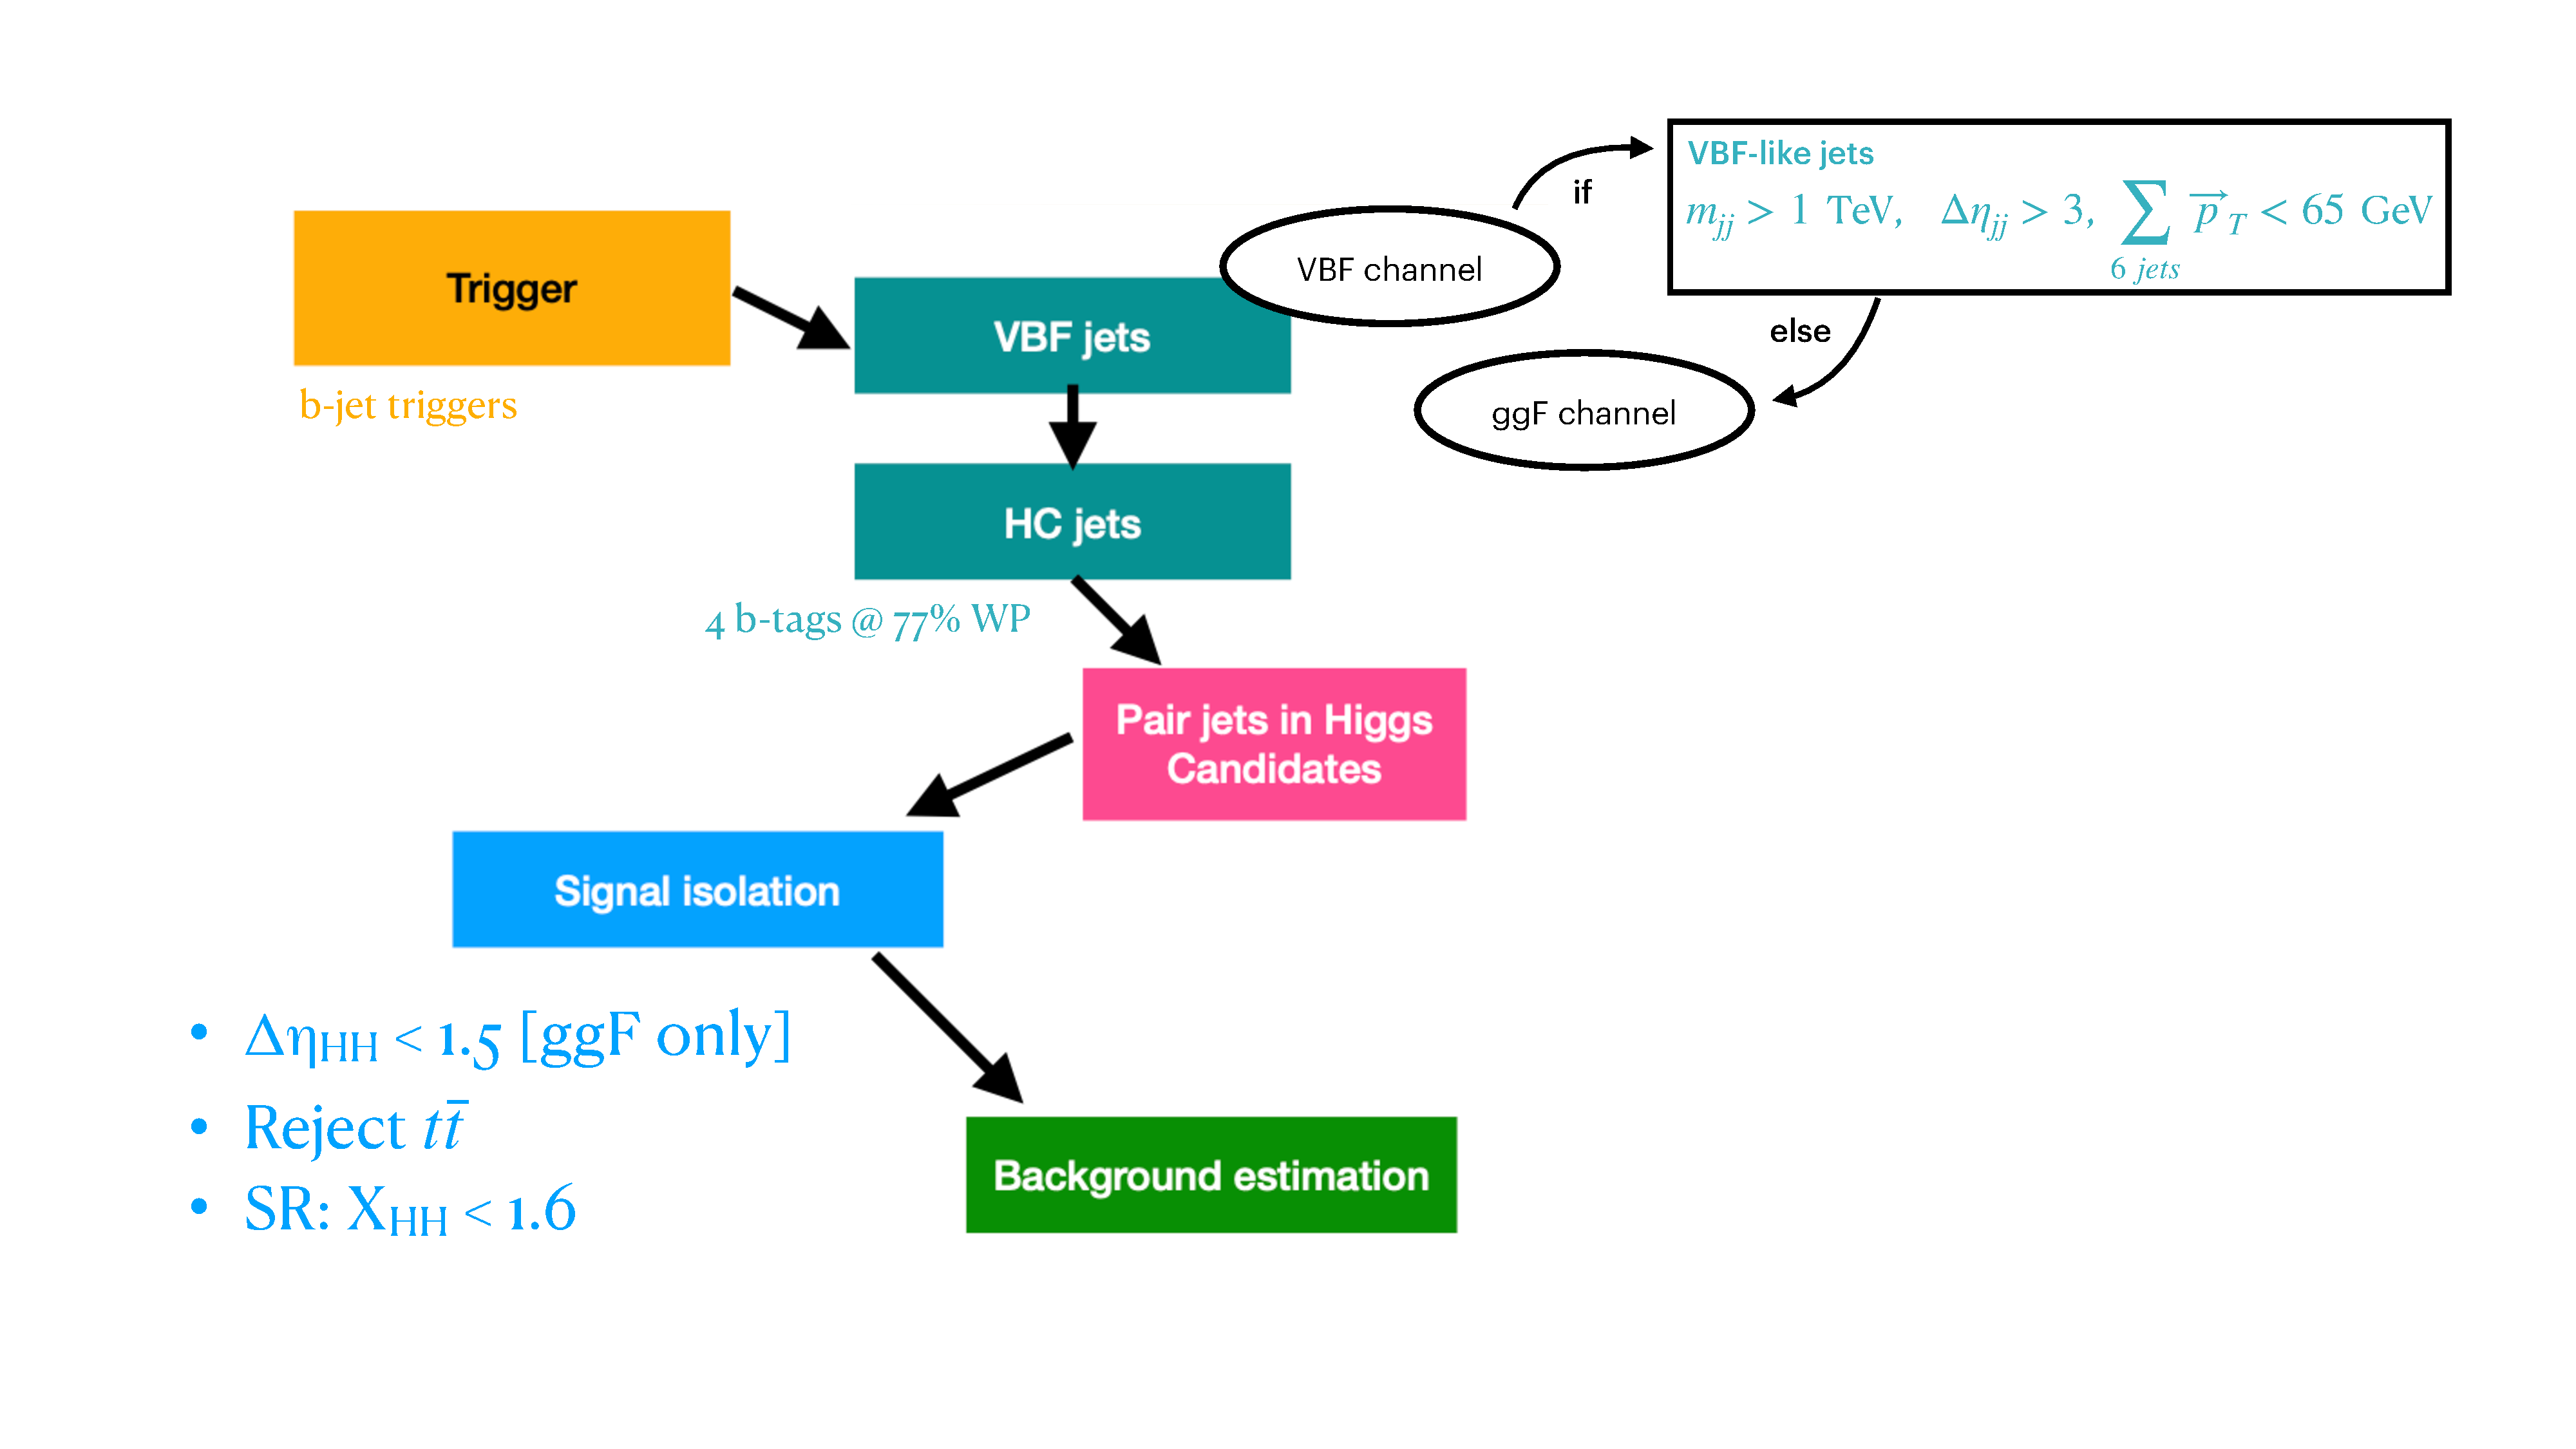
\includegraphics[trim={0 5cm 0 3cm},clip,width=\textwidth]{{figures/my_dihiggs/analysis-overview-graphic.pdf}}
	\caption{Illustration of the high-level analysis strategy.}
	\label{fig:analysis-sel}
\end{figure}

% I might want to describe the offline jet and b-tagging cuts before the trigger section?
Jets are separated into two groups based on their kinematics: 
\begin{description}
	\item[\textit{Central} jets:] $|\eta| < 2.5,\ \pt \ge 40\ \GeV$ -  these jets are used for triggering and will form  Higgs-candidates;
	\item[\textit{Forward} jets:] $|\eta| \ge 2.5,\ \pt \ge 30\ \GeV$ - these extra jets are used to improve the acceptance of jets produced in the vector boson fusion production process.
\end{description}

\subsubsection{\Pqb-jets Selection}
\label{sec:sel-btag}

In order to maximize sensitivity, events are selected and categorized based on the number of \Pqb-tagged \textit{central} jets. 
The \Pqb-tagging algorithm used, DL1r, is described in \Sect{\ref{subsec:ftag}}. 

\paragraph{Ordering and selection} For the jets that form our Higgs Candidates, we take the four leading \Pqb-tagged jets. In events with less than four \Pqb-jets, the extra jets are selected as the highest $p_T$ jets from the pool of \textit{central} jets which failed the initial \Pqb-tag requirement.

\paragraph{\Pqb-tag Requirements} The \Pqb-tag selection for ggF and VBF signals is to require \textbf{at least 4 central jets with DL1r 77\% WP}. Events with two \bjets are classified as 2b events and are used for deriving the data-driven background estimate described in \Sect{\ref{sec:bkgdestimation}}. We also define a systematic on our background estimation using events with 3 \Pqb-tags, and the corresponding \Pqb-tag categories used in this analysis are summarized in table \ref{tab:b-tag-cat}.

\section{Triggers}

\def\figpath{figures/nr-int-note/trigger/V1/}

This analysis uses a combination of multi \Pqb-jet triggers. 
The \pt thresholds and \Pqb-tagging working points vary slightly by the year of data taking ( with the specific cut values delineated in \Tab{\ref{tab:nr-triggers}}).
note - only 2 \Pqb-tags are required in the trigger to avoid creating a bias in the control region used in the background estimation that will be described in \Sect{\ref{sec:rw-overview}}.
The \Pqb-tagging SFs are derived for each trigger chain individually required our analysis strategy to specify which trigger stream was considered for the trigger SF application.
One other interesting feature of our analysis is our signal is not fully efficient for our analysis, as illustrated by efficiencies that are less than 100\% in Fig{\ref{fig:HH_trigger_eff}}, and also this efficiency is varying as a function of the reconstructed 4-jet invariant mass. 
 
\begin{table}[htbp]
\centering
\begin{tabular}{p{2cm}  p{1cm} | p{6cm}  | p{4.5cm} }
\textbf{Trigger Type} & Year & HLT thresholds & L1 thresholds \\
\hline
{} & 2016 & \small{ $\pt > 100$~GeV jet \& two $\pt > 55$~GeV 60\%~WP \Pqb-jets } &  \small{ five $\pt > 15$~GeV jets} \\
\textbf{2b1j} & 2017 &  \small{ $\pt > 150$~GeV jet \& two $\pt > 55$~GeV 70\%~WP \Pqb-jets }&  \small{ $\pt > 85$~GeV jet \& two $\pt~>~30$~GeV jets } \\
{} & 2018 &  \small{ $\pt > 150$~GeV jet \& two $\pt > 55$~GeV 70\%~WP \Pqb-jets }&  \small{ $\pt > 85$~GeV jet \& two $\pt~>~30$~GeV jets }\\
\hline
{} & 2016 &  \small{ four $\pt > 35$~GeV jets, two 60\% WP \Pqb-tags} & {} \\ 
\textbf{2b2j} & 2017 &  \small{four  $\pt > 35$~GeV jets, two 40\% WP \Pqb-tags} &  \small{four $\pt > 15$~GeV,  $|\eta| < 2.5$ jets} \\
{} &  2018 &  \small{four $\pt > 35$~GeV jets, two 60\% WP \Pqb-tags}  & {} \\
\end{tabular}
\caption{Triggers used for non-resonant searches. For \Pqb-tagging in the trigger in Run 2, the MV2 version of the \Pqb-tagger is used. Also, an L1 $|\eta| < 3.2$ cut is assumed where not specified.}
\label{tab:nr-triggers}
\end{table}

\begin{figure}[htb]
        \centering
                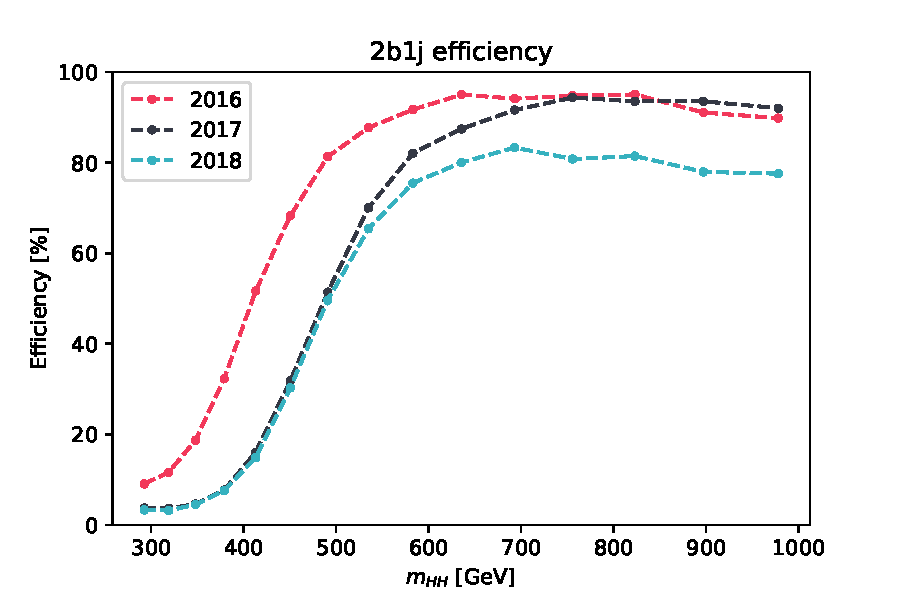
\includegraphics[width=0.32\textwidth]{\figpath/SMNR_ggF_600043-2b1j-trigger-efficiency.pdf}
                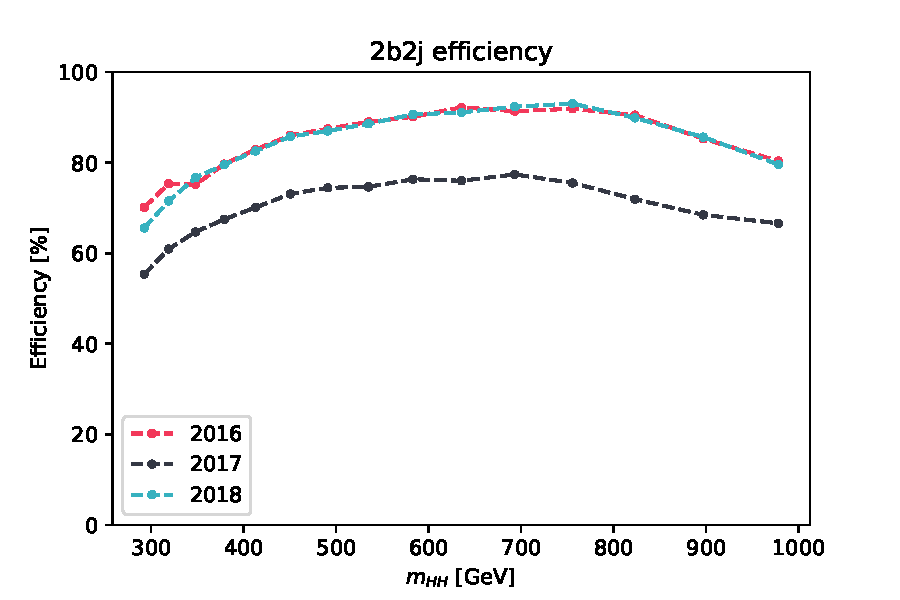
\includegraphics[width=0.32\textwidth]{\figpath/SMNR_ggF_600043-2b2j-trigger-efficiency.pdf}
                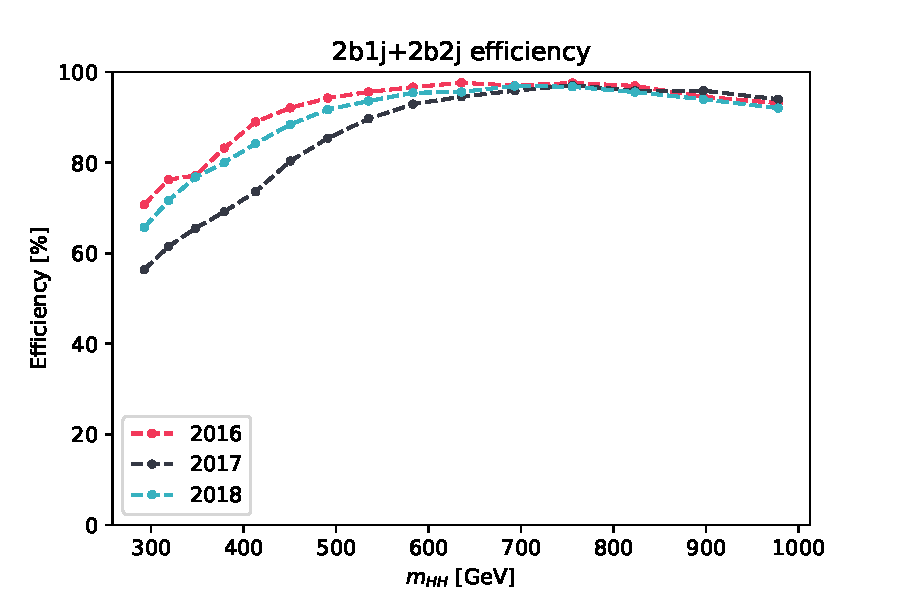
\includegraphics[width=0.32\textwidth]{\figpath/SMNR_ggF_600043-2b1j+2b2j-trigger-efficiency.pdf}
        \caption{Trigger efficiencies of the 2b1j, 2b2j and combined for the MC16a/d/e corresponding to years 2016-2018 for the SM ggF \kl=1 signal.
        Significantly lower efficiency for 2017 2b2j comparing to other years is due to tighter b-tagging requirement (lower efficiency). \hl{Is this plot inside of the SR?}}
	\label{fig:HH_trigger_eff}
\end{figure}

To account for this feature of ``operating on the turn on curve'' the SF that we apply to account for the trigger effects 

%%%%%%%%%%%%%%%%%%%%%%%%%%%%%%%
\subsection{Trigger buckets}
%%%%%%%%%%%%%%%%%%%%%%%%%%%%%%%

To distinguish which trigger chain to check, we cut on the offline jets $p_{\text{T},1} > 170$~GeV and $p_{\text{T},3} > 70$~GeV, where the jets are ordered by \pt.
These jet \pt cuts mimic the 2b1j trigger.
If the event passes these jet cuts, we put it in trigger \textbf{bucket 1}, otherwise it goes in trigger \textbf{bucket 2}.
In trigger bucket 1, we check the decision of the 2b1j trigger to decide whether to keep the event, and in trigger bucket 2, we check the 2b2j trigger. This procedure is summarized graphically in \Fig{\ref{fig:trigger-bucket-strategy}}.

\begin{figure}[htbp]
    \centering
    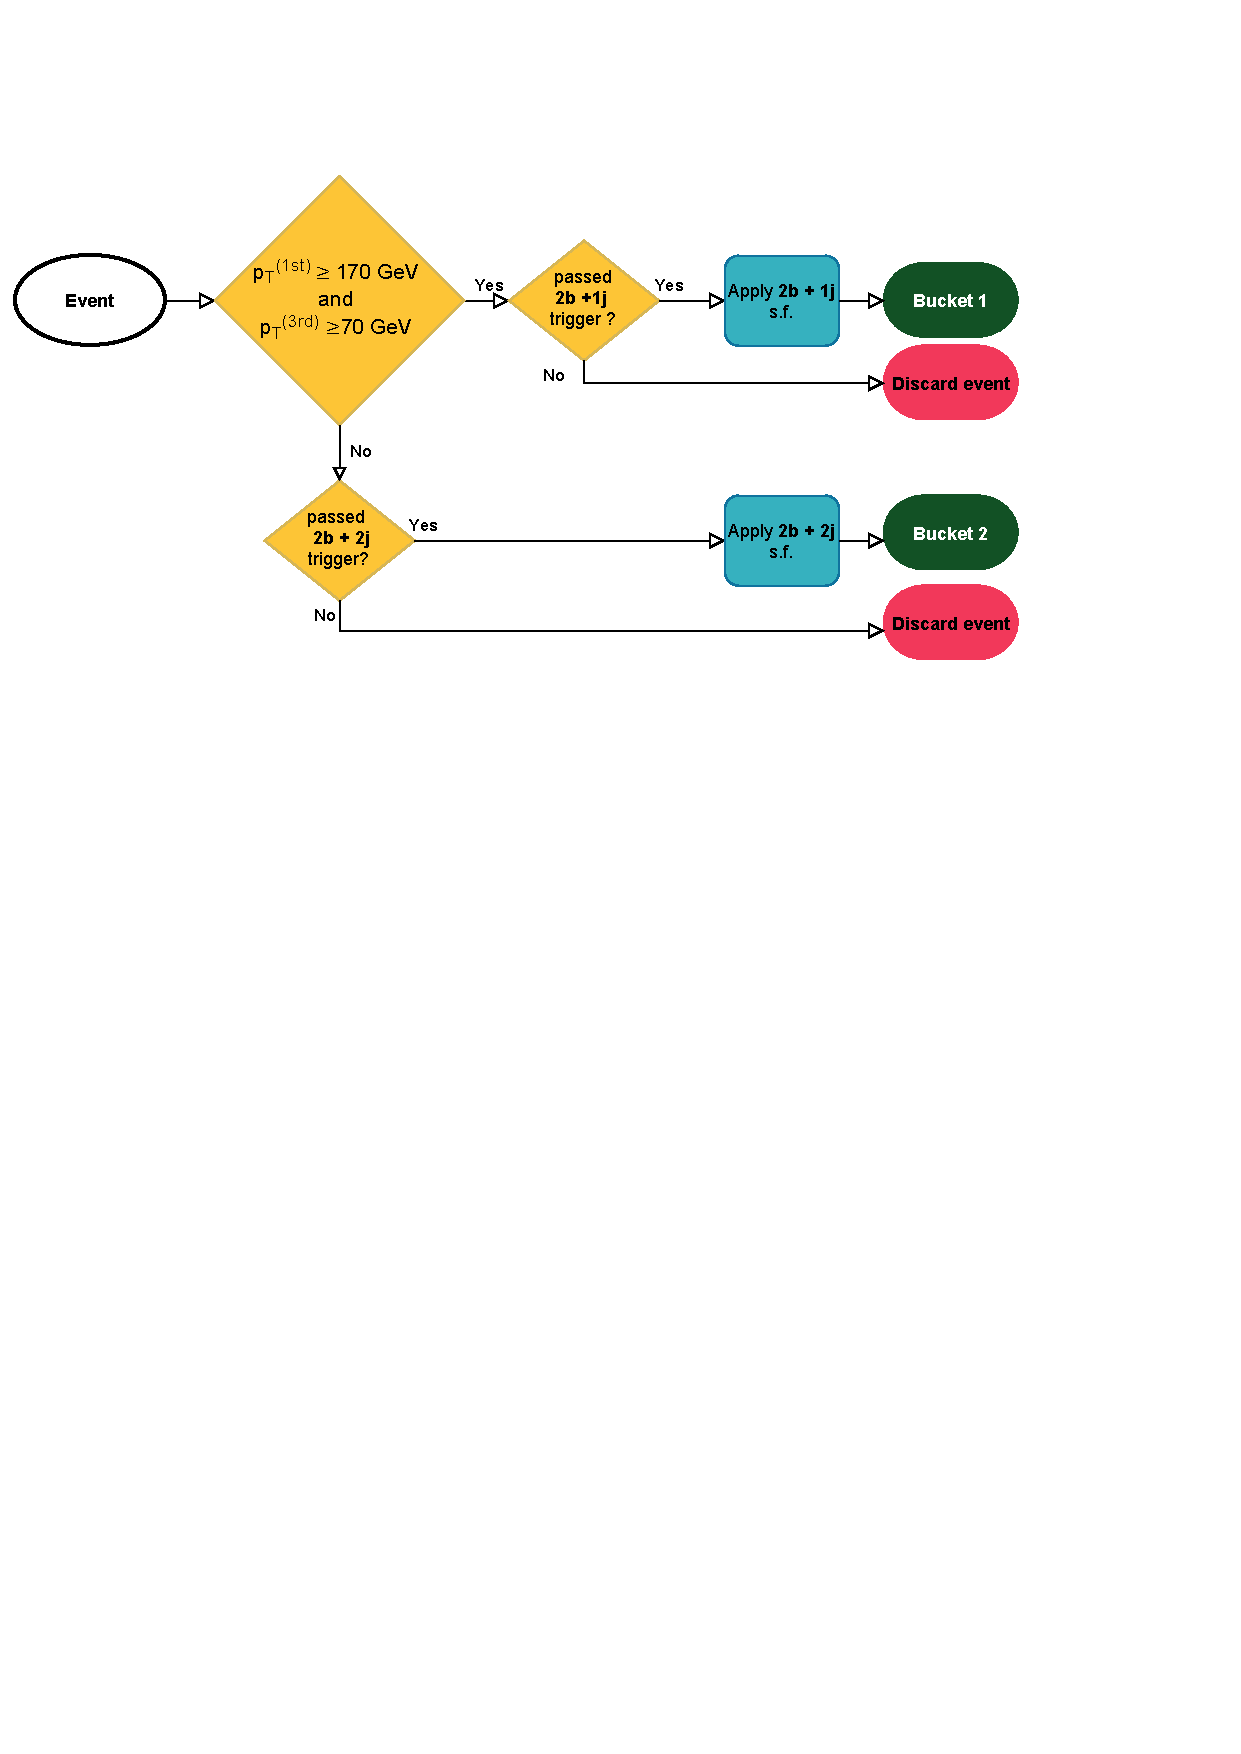
\includegraphics[width=0.8\textwidth]{\figpath/nr_buckets_diagram_simple.pdf}
    \caption{Trigger bucket strategy for non-resonant searches.}
    \label{fig:trigger-bucket-strategy}
\end{figure}

\Fig{\ref{fig:trig-bucket-4b}} shows how this strategy of using a combination of two triggers gives us sensitivity to complementary phase spaces in the analysis. The 2b1j trigger drives our acceptance for the high \mhh events, while the 2b2j trigger provides our low \mhh acceptance.

\begin{figure}
    \centering
    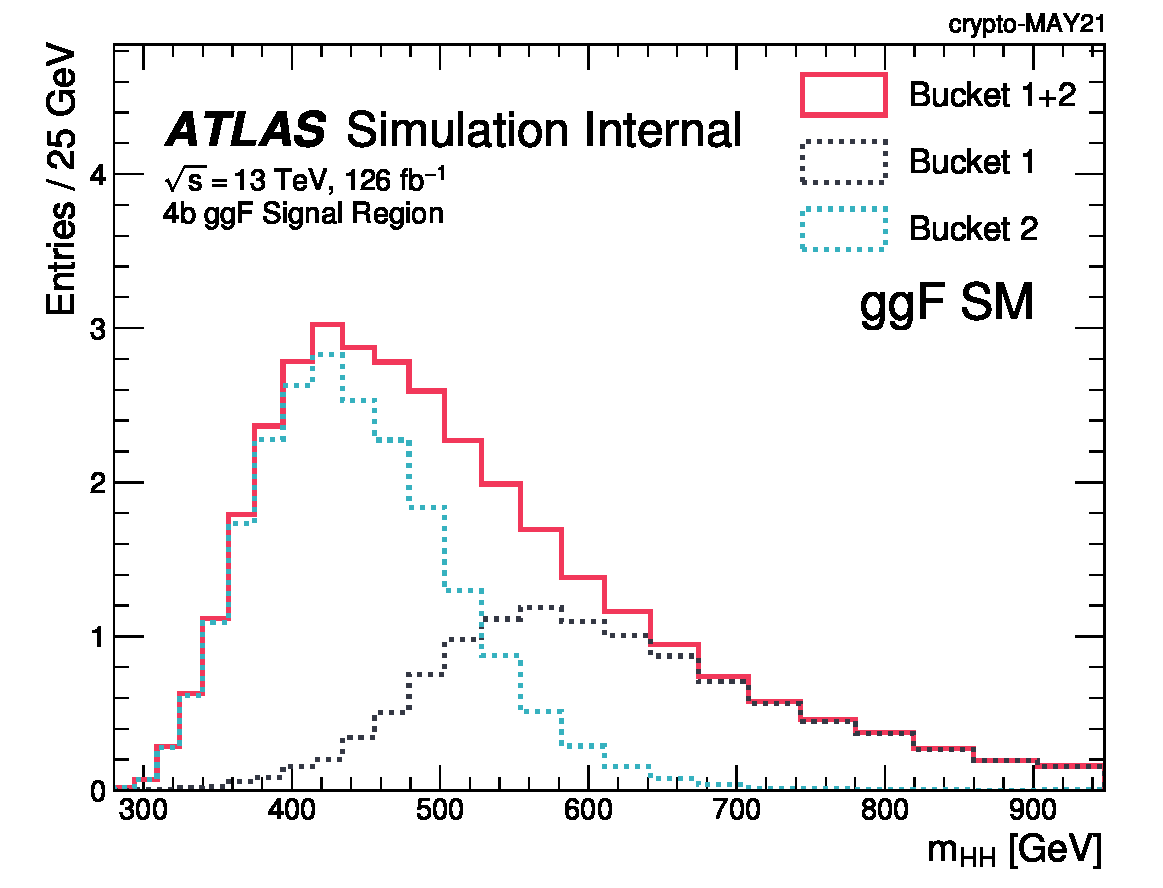
\includegraphics[width=0.48\textwidth]{\figpath/buckets_comparison_4b_ggF_SM_SR.pdf}
    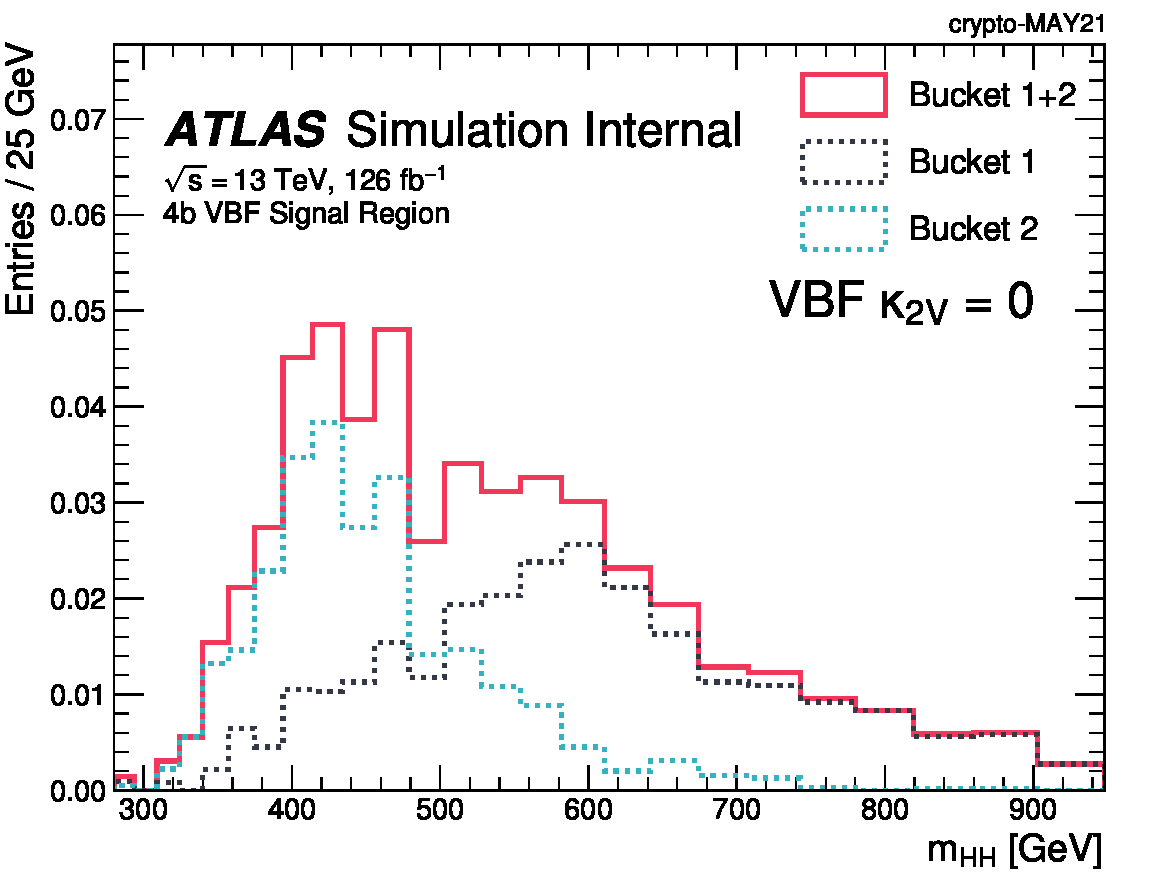
\includegraphics[width=0.48\textwidth]{\figpath/buckets_comparison_4b_VBF_SR.pdf}
    \caption{The bucket composition of \mhh for the SM ggF (left) and \kvv = 0 VBF (right) \HH MC simulation in the 4b Signal Regions.  Bucket 1 corresponds to the 2b1j trigger and Bucket 2 corresponds to the 2b2j trigger.}
    \label{fig:trig-bucket-4b}
\end{figure}

To reconstruct the trigger decision and define the jet level SFs, offline jets are matched to the online jets using a $\Delta R$matching criterion.
% There are different cuts being used:
% - dR < 0.4 for defining the trigger match and applying the CDI SFs
% - dR < 0.3 for deriving the HLT ET SFs
% - dR < 0.4 for deriving the L1 ET SFs
% but I'm not sure if dR < 0.4 is always used for applying these SFs
These online jets are then checked to pass the (online) thresholds given in Table~2, and if this many jets and \Pqb-jets pass this selection, the event passes this trigger. 
For ease of knowing how to apply the SFs, we will only keep events where the trigger passed in the relevant bucket, i.e, the 2b1j trigger needs to pass if the event passed the offline cuts in bucket 2, and the 2b2j trigger needs to pass if the event passed the offline cuts in bucket 1.
The event level trigger SF is calculated from the jet level SFs (\Eq{\ref{eq:trig-sf-all}}) with two contributions:

\begin{equation}
\text{Multi \Pqb-jet trigger SF} = \prod_i \textcolor{dodgerblue}{  SF_{jet}^{b-tag}(i)} \times \textcolor{orange}{SF_{jet}^{kinematic}(i)}  
\label{eq:trig-sf-all}
 \end{equation}

\begin{itemize}
\item \textcolor{dodgerblue}{ \Pqb-jet trigger SFs using prescription from by the \Pqb-jet trigger group (described in \Sect{\ref{subsec:trig-sf-bjet}})}
%(although they were customly rederived down to 30 GeV since we were investigating a low \pT category).}
\item  \textcolor{orange}{ Kinematic $E_\text{T}$ HLT and L1 SFs derived in a custom $t\bar{t}$ analysis (described in \Sect{\ref{subsec:trig-sf-et}})}
\end{itemize}

%%%%%%%%%%%%%%%%%%%%%%%%%%%%%%%
\subsection{b-jet SF}
\label{subsec:trig-sf-bjet}
%%%%%%%%%%%%%%%%%%%%%%%%%%%%%%%

The offline and online \Pqb-tagging decisions are highly correlated, so the online \Pqb-tagging SF are derived conditional based on the offline \Pqb-tagging decision. 
Since both the offline and online $\Pqb$-tagging decisions could pass or fail, this gives four cases:

\begin{itemize}
\setlength\itemsep{-1.5em}
   \item Case 1: Pass online and offline \Pqb-tagging: 
   	\vspace{-1em}
	  \begin{equation*}
		 \varepsilon(\text{on} \land \text{off}) 
		 = \varepsilon(\text{on} | \text{off}) \varepsilon(\text{off})
	  \end{equation*}
   \item Case 2: Fail the online \Pqb-tag, but pass the offline \Pqb-tag: 
   	\vspace{-1em}
	  \begin{equation*}
		 \varepsilon(\overline{\text{on}} \land \text{off}) 
		 = [1 - \varepsilon(\text{on} | \text{off})] \varepsilon(\text{off})
	  \end{equation*}
   \item Case 3: Pass the online \Pqb-tag, but fail the offline \Pqb-tag: 
   	\vspace{-1em}
	  \begin{equation*}
		 \varepsilon(\text{on} \land \overline{\text{off}}) 
		 = \varepsilon(\text{on}) - \varepsilon(\text{on} | \text{off}) \varepsilon(\text{off})
	  \end{equation*}
   \item Case 4: Fail the online and offline \Pqb-tagging: 
   	\vspace{-1em}
	  \begin{equation*}
		 \varepsilon(\overline{\text{on}} \land \overline{\text{off}}) 
		 = 1 - \varepsilon(\text{off}) - \varepsilon(\text{on}) + \varepsilon(\text{on} | \text{off}) \varepsilon(\text{off})
	  \end{equation*}
\end{itemize}

Then for each efficiency, we still apply $SF = \varepsilon^{data} / \varepsilon^{MC}$.
For offline jets that are not matched to a corresponding online HLT jet, just the offline SF is applied, just the offline \Pqb-tagging SF is applied, as visualized in \Fig{\ref{fig:ftag-online-sf}}.

\begin{figure}
\centering
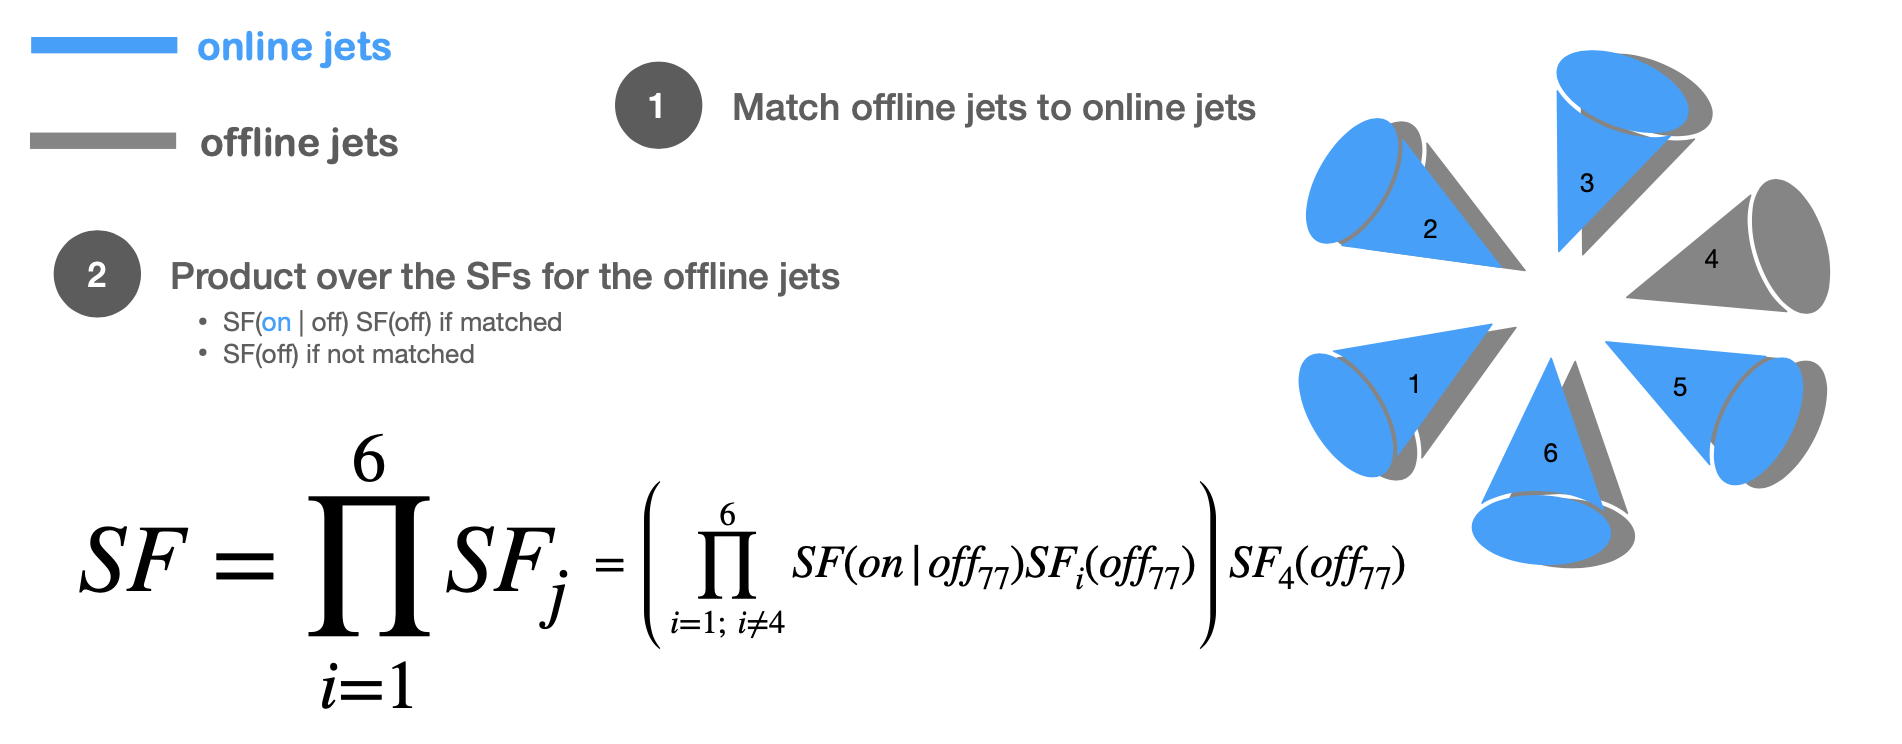
\includegraphics[width=\textwidth]{figures/my_dihiggs/check-btag-jets-sf.png}
\caption{Illustration of how the combined offline / online \Pqb-tagging SF is calculated.}
\label{fig:ftag-online-sf}
\end{figure}

Our use of the \Pqb-jet triggers dictates SFs dictates how much of the Run~2 dataset we can use.
\begin{enumerate}
\item In 2016 there was an issue in the online beam spot calculation, which impacted the primary vertex calculation for the HLT \Pqb-tagging. Because of this, we don't use this portion of the data from the 2016 dataset, a loss of 8.3~\ifb from the 32.8~\ifb of the full 2016 dataset.
\item Even for 2017 and 2018, we need to discard the first luminosity blocks of data taking where the beam spot has not yet had time to update. This means analyses with \Pqb-jet triggers have $\approx 1.5$\% lower luminosity in these years than the baseline luminosity \cite{b-trig-paper}.
\item The astute reader might notice that the 2015 triggers are not included in \Tab{\ref{tab:nr-triggers}}. As will be explained in \Sect{ch:bkg-est}, the background estimate is derived for each year separately to account for the differences in the trigger, and the robustness of the background estimate is partially based on the size of the sample used to derive it. Since it wasn't clear whether the 2015 dataset was large enough to warrant the gains of the additional complexity in the analysis, the 2015 conditional \Pqb-jet trigger SFs were never derived with respect to the offline DL1r algorithm, so this year of data is not included.
%Although the 2015 data was included in the partial Run~2 analysis \cite{paper-4b-36ifb}, in the intervening years ATLAS revamped the offline \Pqb-tagging software - and the conditional online SFs were not rederived with respect to the online \Pqb-tagger.
\end{enumerate}

In summary, when accounting for the above three points, \Tab{\ref{tab:lumi-yr}} is the (by year) luminosity for the 4b analysis, with a total luminosity is 126.0~\ifb. %, $\approx 10$\% lower than the 139~\ifb for analyses that don't need \Pqb-jet triggers.

\begin{table}[htbp]
\centering
\begin{tabular}{| c | c |}
\hline
\textbf{Year} & \textbf{Luminosity}  [\ifb] \\
\hline
2016 & 24.6 \\
2017 & 43.7 \\
2018 & 57.7 \\
\hline
all & 126.0 \\
\hline
\end{tabular}
\caption{Luminosty (by year) for the 4b analysis.}
\label{tab:lumi-yr}
\end{table}

%%%%%%%%%%%%%%%%%%%%%%%%%%%%%%%
\subsection{Kinematic SF}
\label{subsec:trig-sf-et}
%%%%%%%%%%%%%%%%%%%%%%%%%%%%%%%

\hl{Q that I have -- how do we apply the jet level SFs? Do we multiply over all of the offline jets in the event, but these are only non-unary for the first $N$ jets ordered by online ET?}

\begin{figure}[ht]
    \centering
    \subfloat[1st jet at L1]{\label{fig:jet-level-trigSF17-2b1j-L1-1st}
            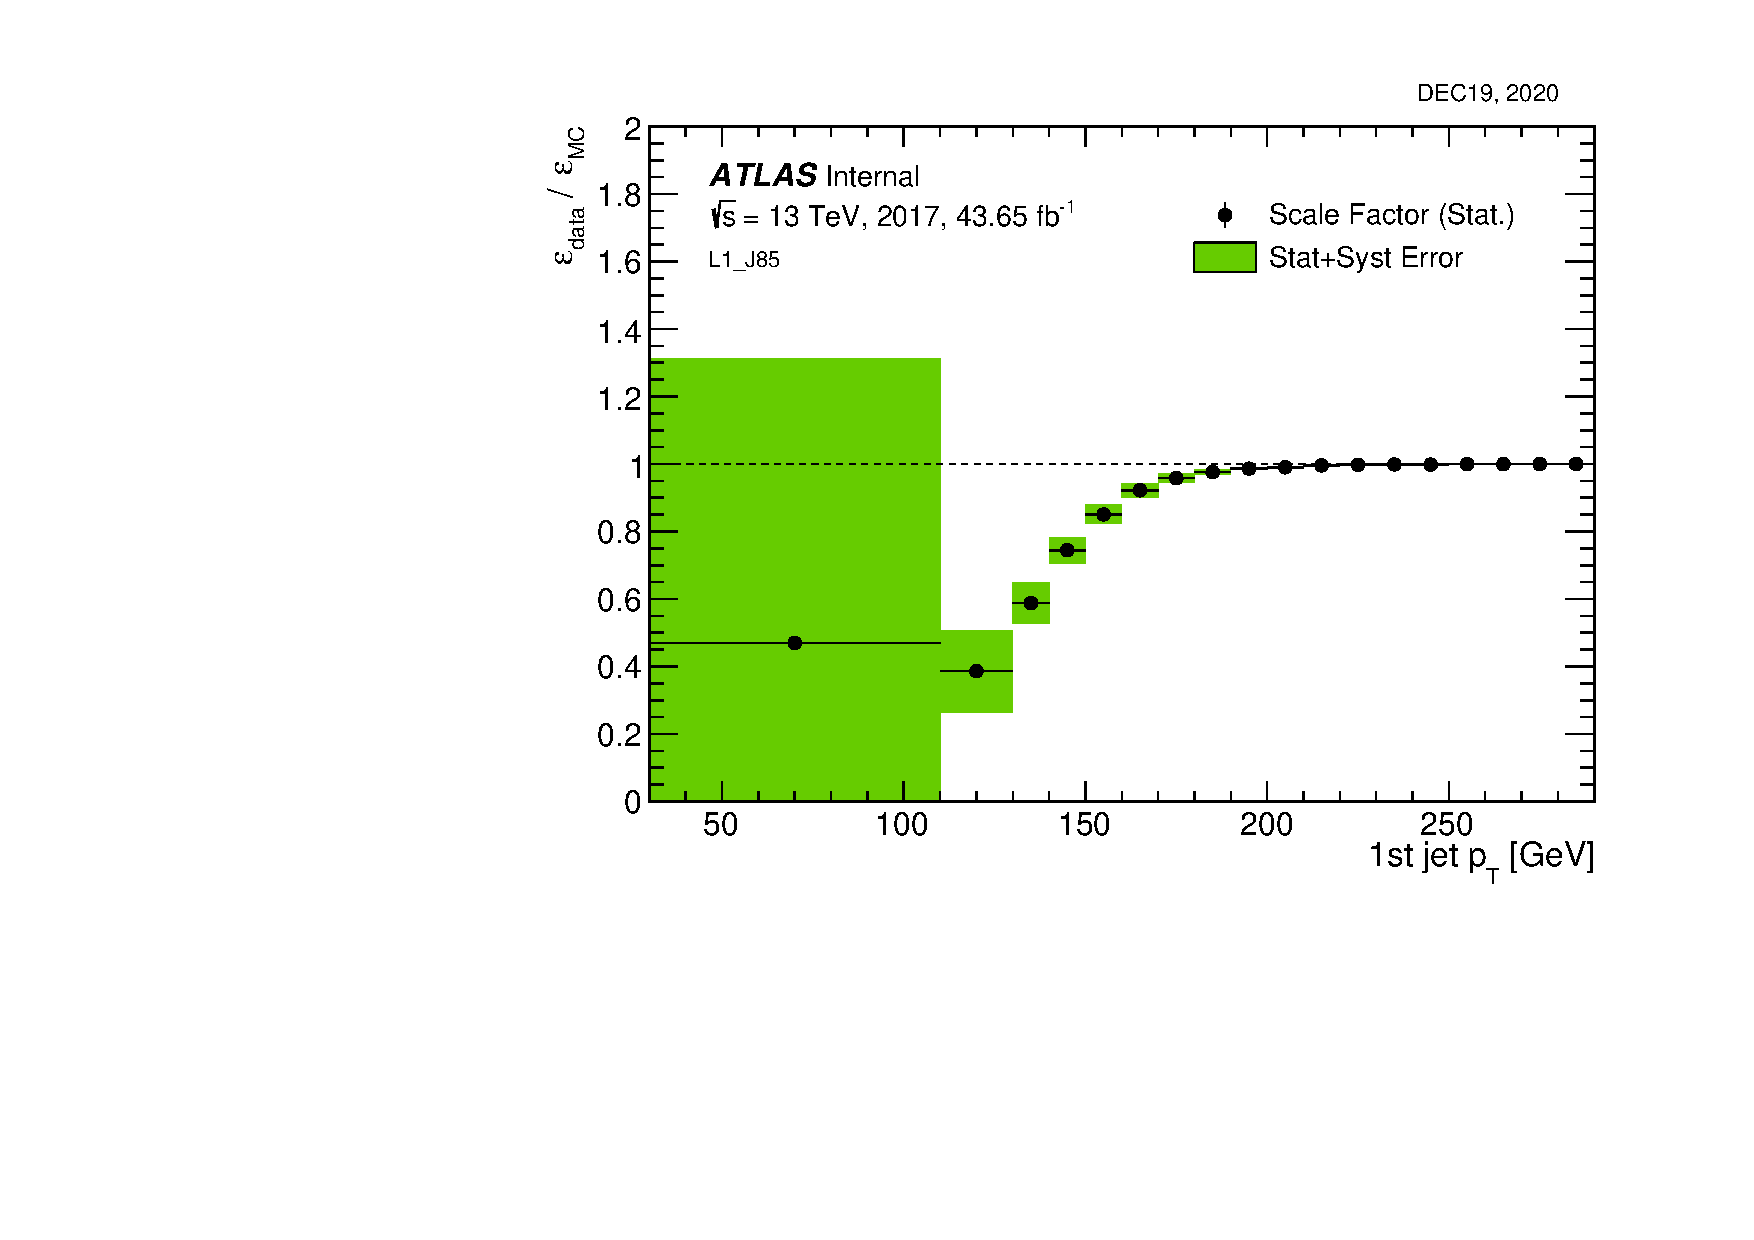
\includegraphics[width=0.3\textwidth]{figures/nr-int-note/appendices/jet-level-trigger-sf/V1/L1SF/2017/trigSF17-2b1j-L1-1st.pdf}
    }
    \subfloat[2nd jet at L1]{\label{fig:jet-level-trigSF17-2b1j-L1-2nd}
            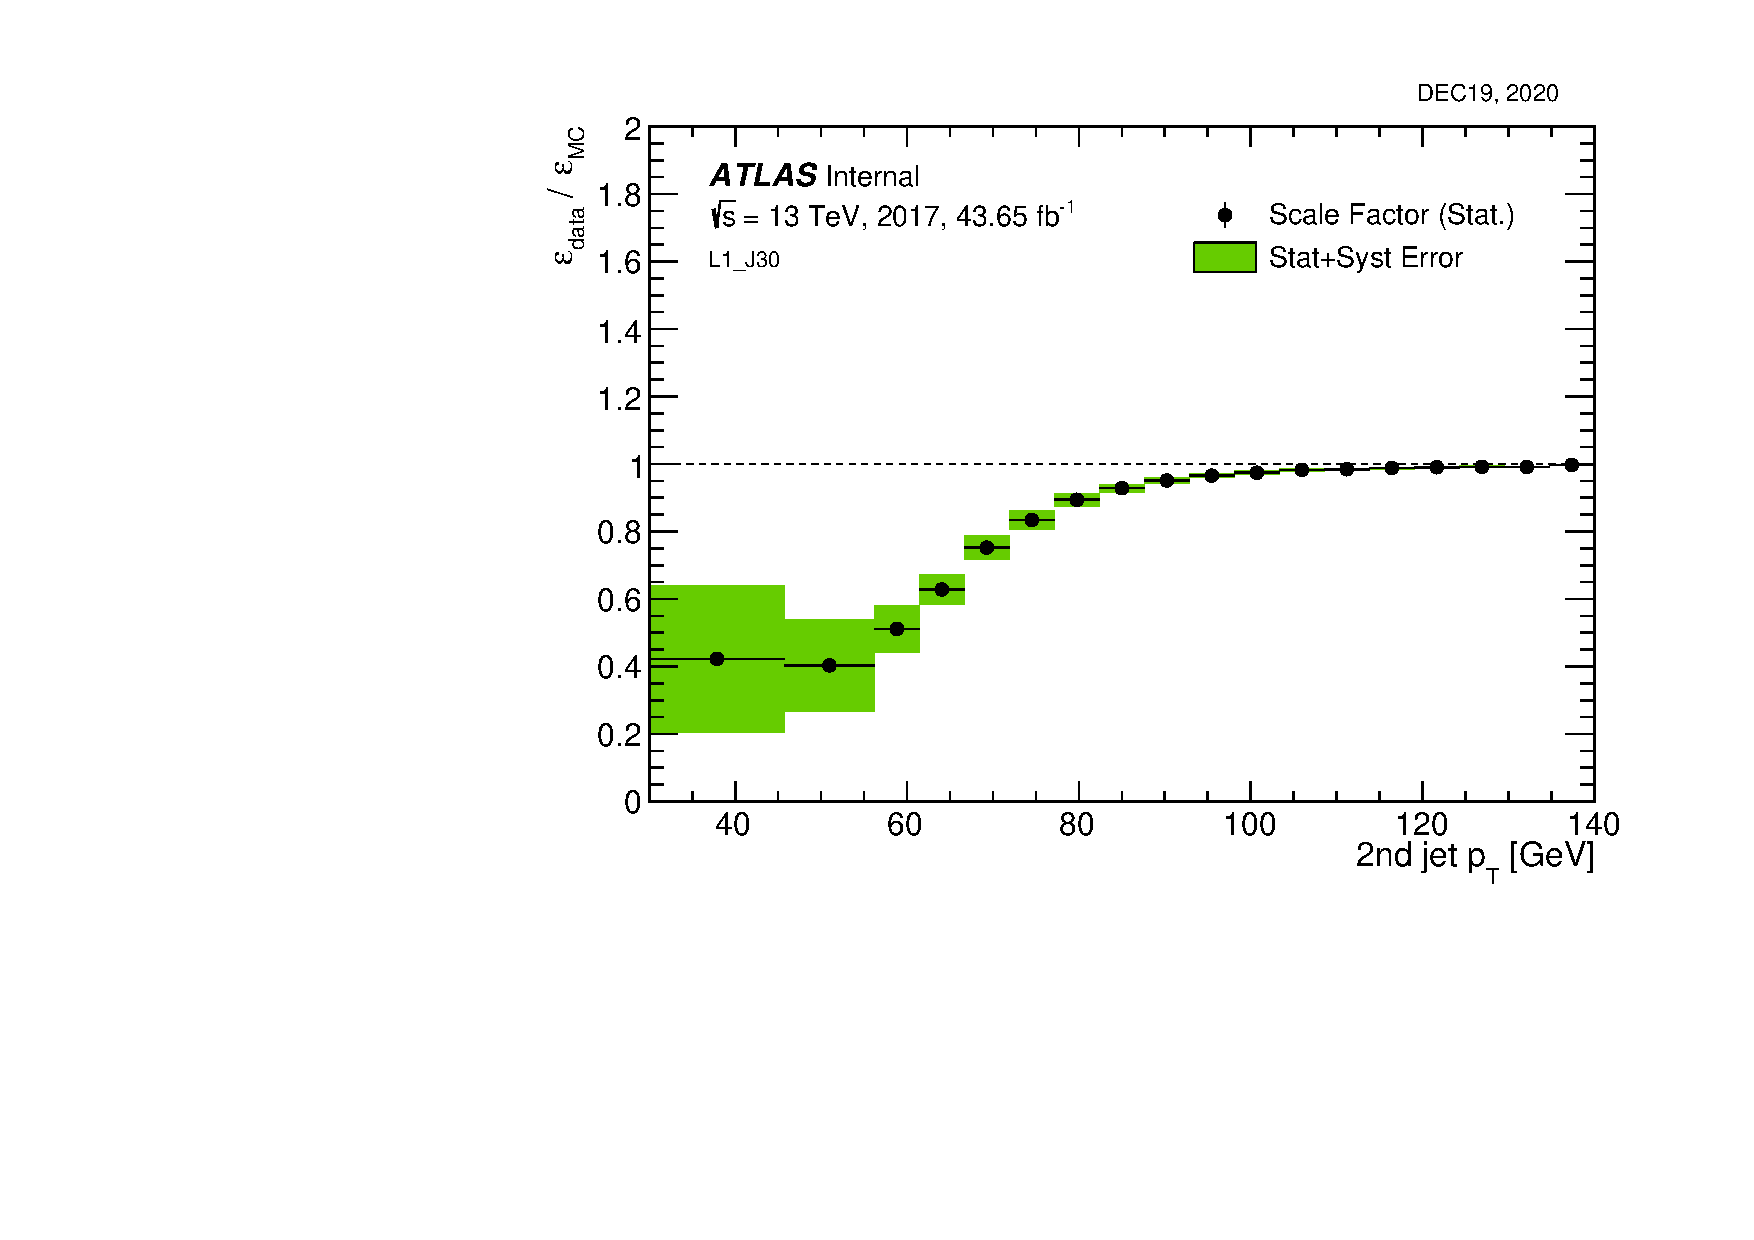
\includegraphics[width=0.3\textwidth]{figures/nr-int-note/appendices/jet-level-trigger-sf/V1/L1SF/2017/trigSF17-2b1j-L1-2nd.pdf}
    }
    \subfloat[3rd jet at L1]{\label{fig:jet-level-trigSF17-2b1j-L1-3rd}
            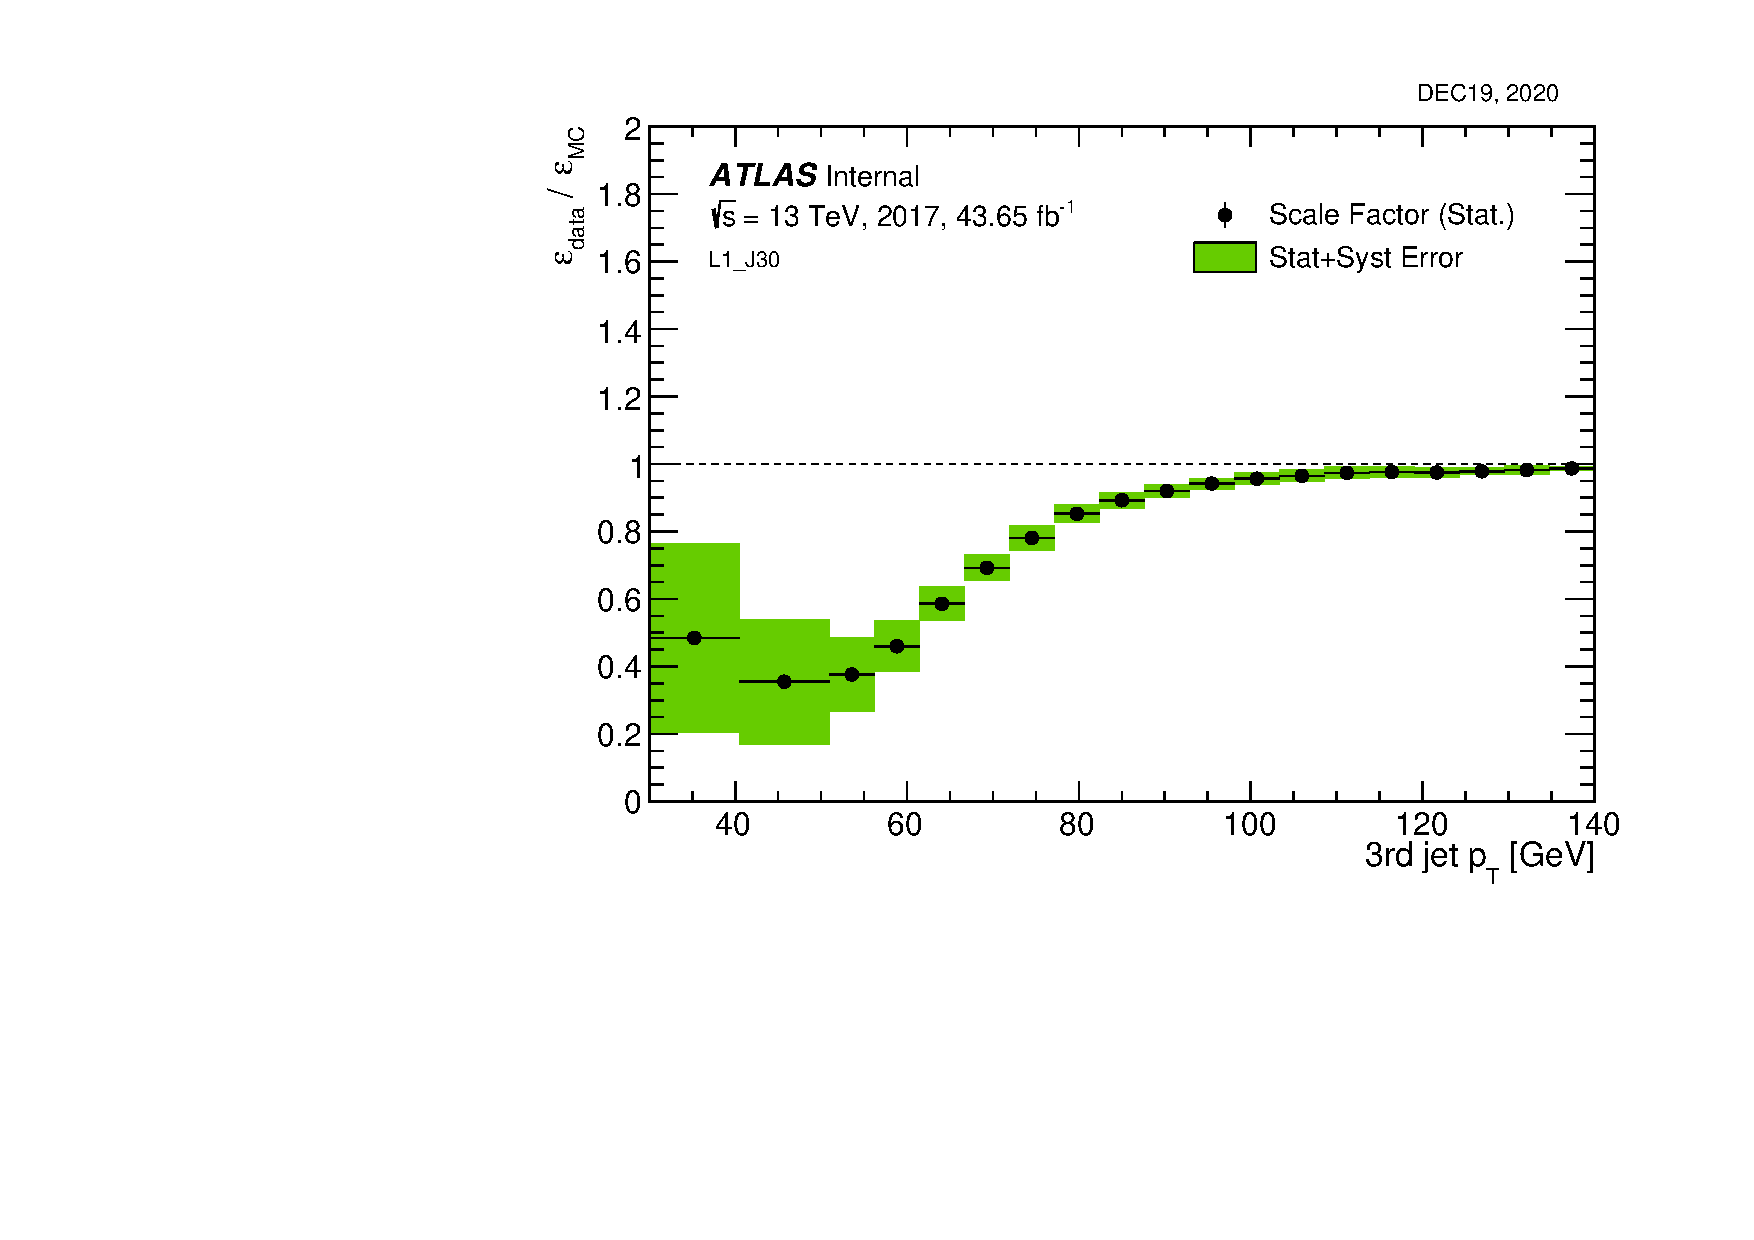
\includegraphics[width=0.3\textwidth]{figures/nr-int-note/appendices/jet-level-trigger-sf/V1/L1SF/2017/trigSF17-2b1j-L1-3rd.pdf}
    }

    \subfloat[1st jet at HLT]{\label{fig:jet-level-trigSF17-2b1j-HLT-1st}
            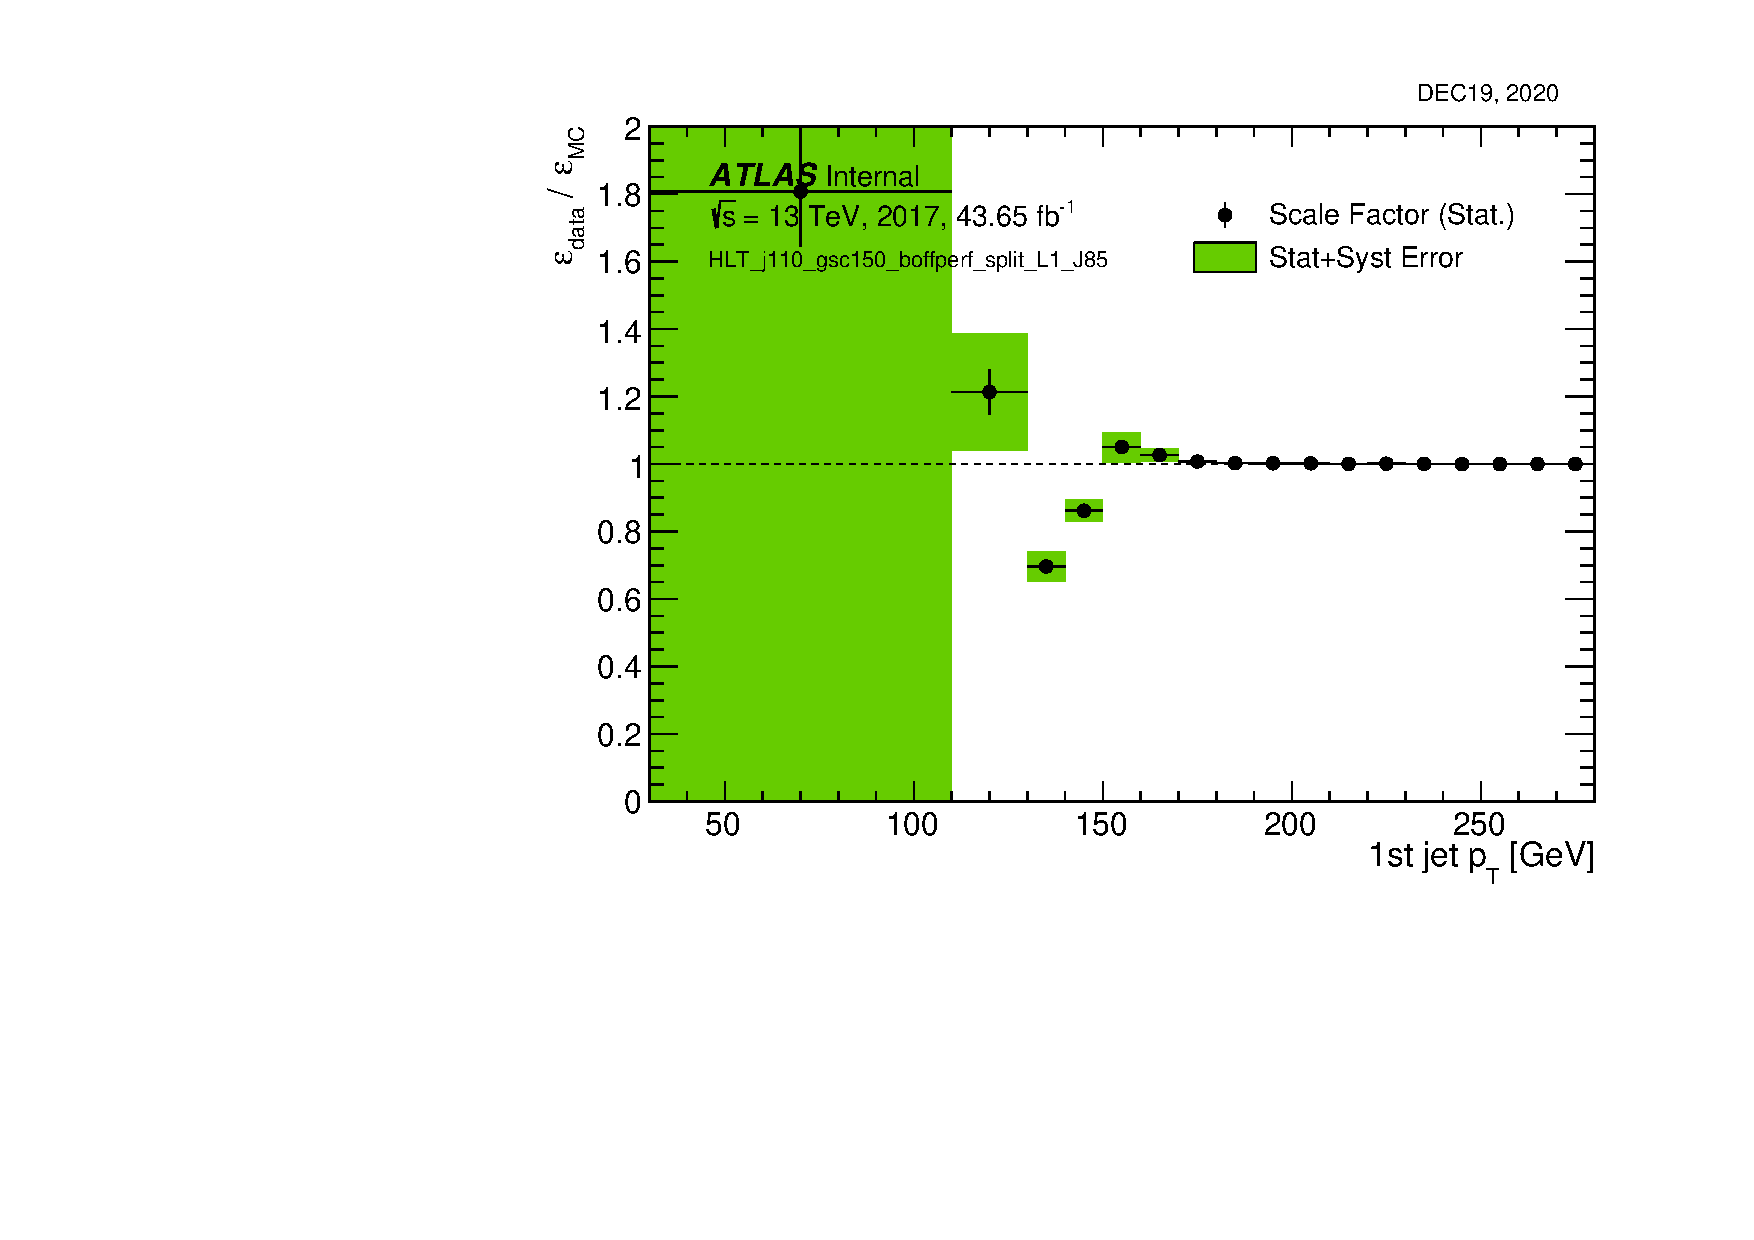
\includegraphics[width=0.3\textwidth]{figures/nr-int-note/appendices/jet-level-trigger-sf/V1/HLTSF/2017/trigSF17-2b1j-HLT-1st.pdf}
    }
    \subfloat[2nd jet at HLT]{\label{fig:jet-level-trigSF17-2b1j-HLT-2nd}
            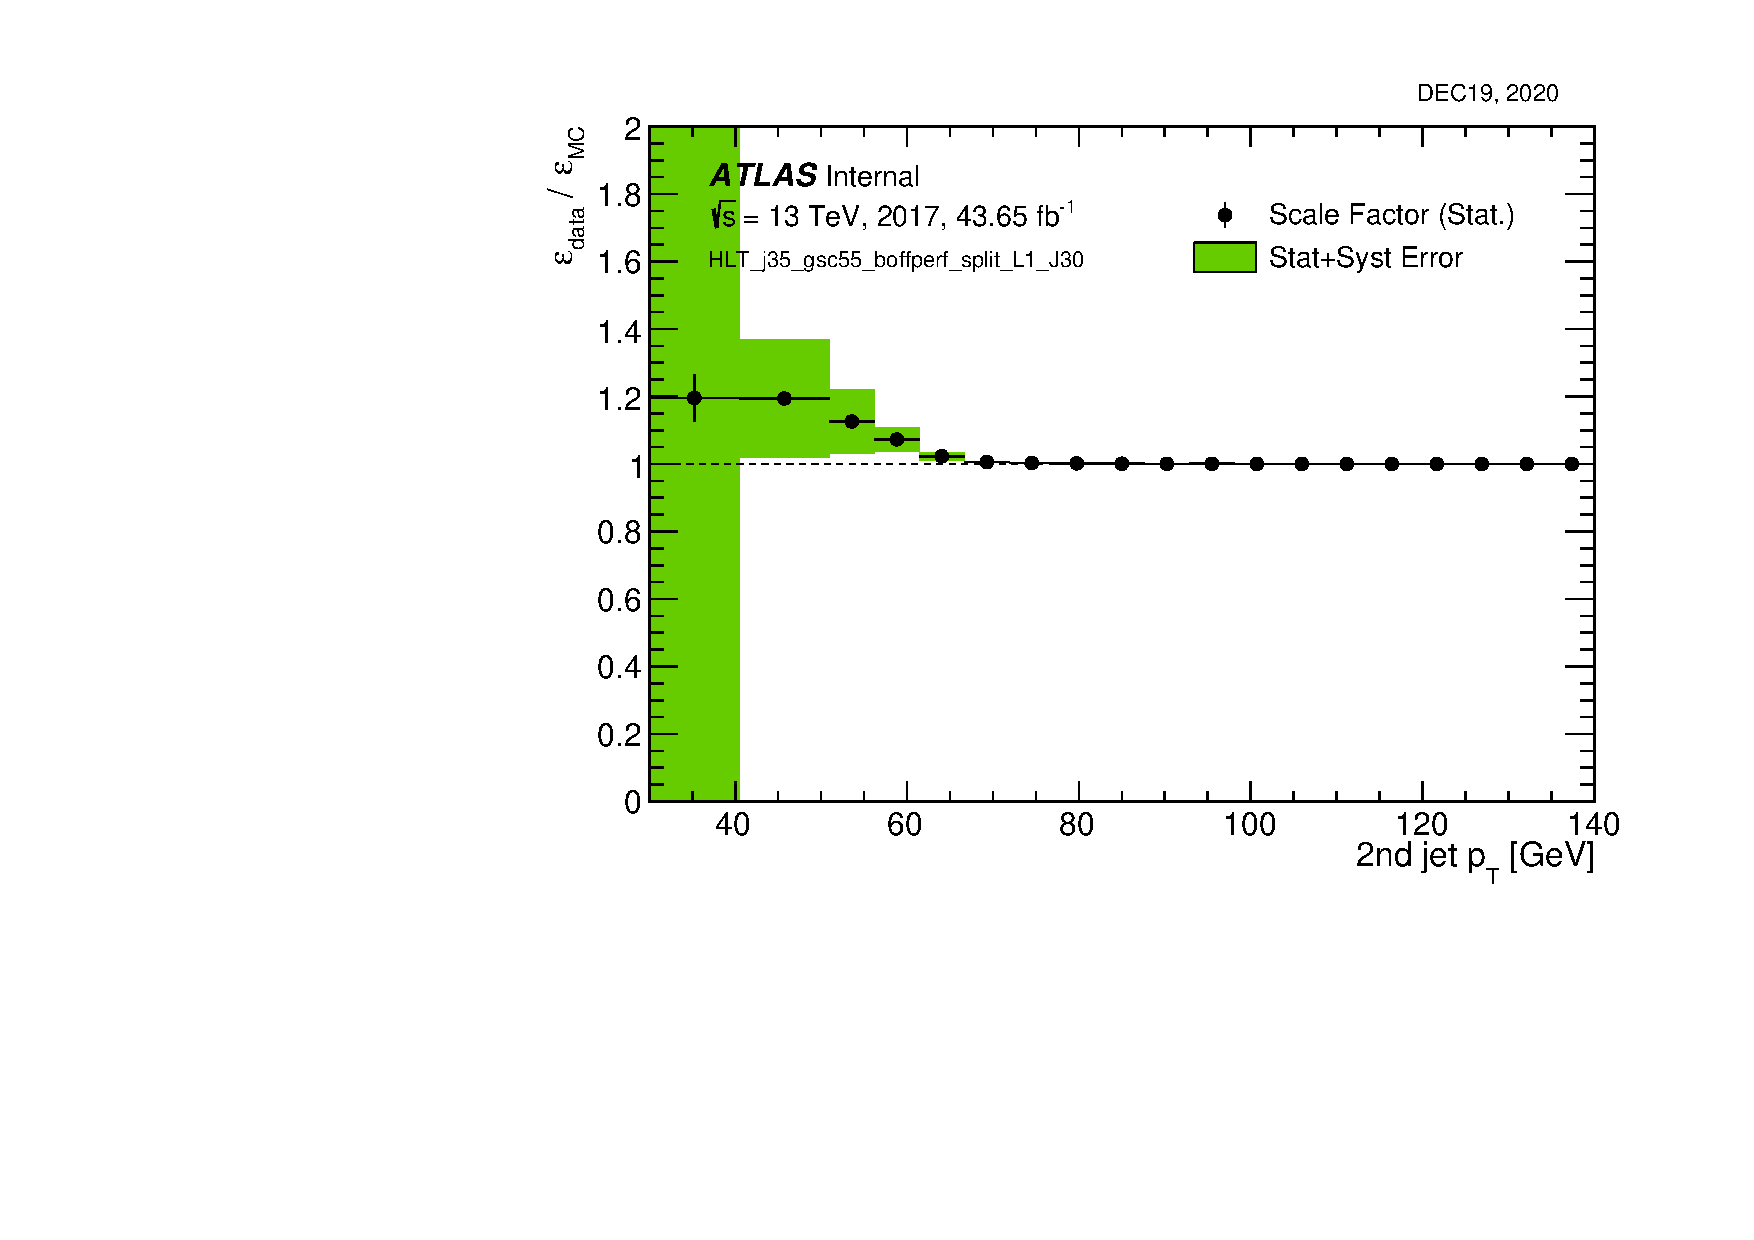
\includegraphics[width=0.3\textwidth]{figures/nr-int-note/appendices/jet-level-trigger-sf/V1/HLTSF/2017/trigSF17-2b1j-HLT-2nd.pdf}
    }
    \subfloat[3rd jet at HLT]{\label{fig:jet-level-trigSF17-2b1j-HLT-3rd}
            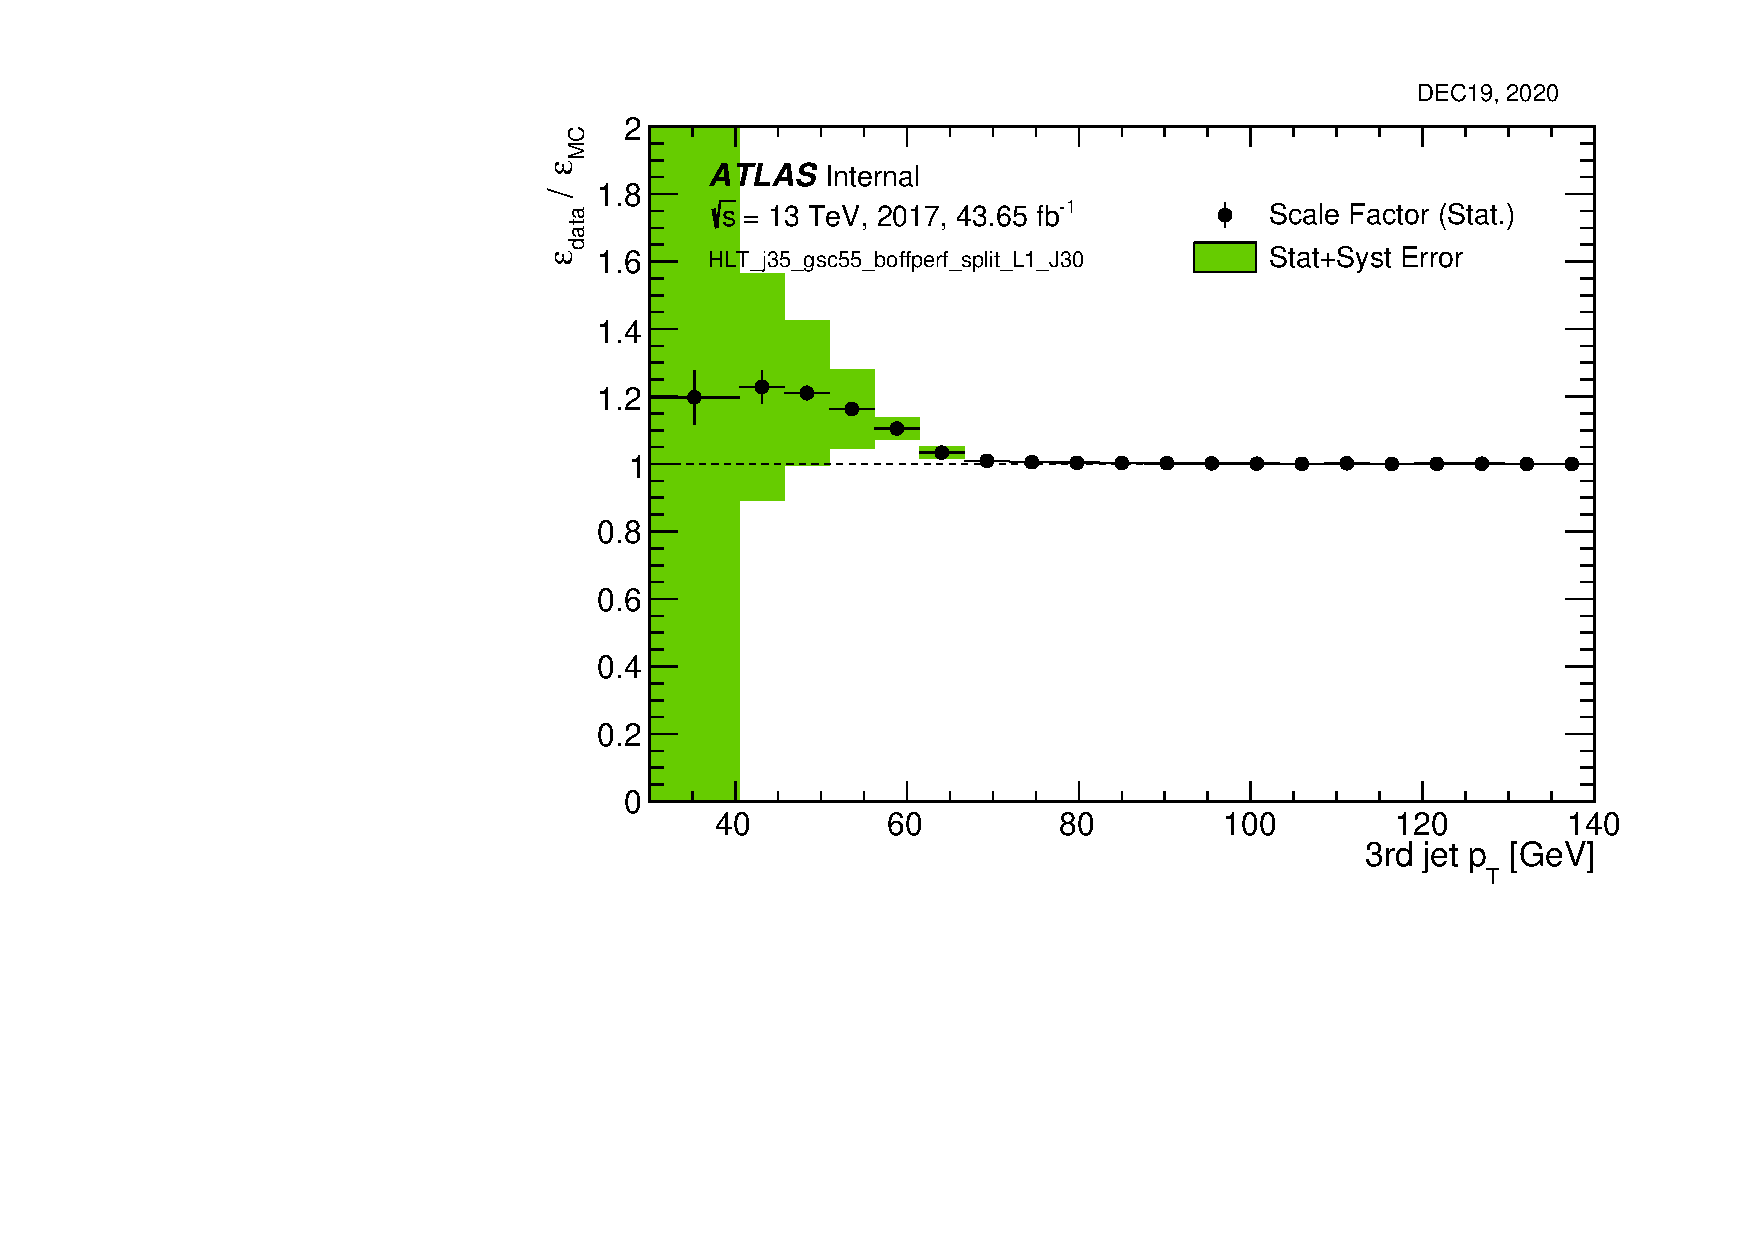
\includegraphics[width=0.3\textwidth]{figures/nr-int-note/appendices/jet-level-trigger-sf/V1/HLTSF/2017/trigSF17-2b1j-HLT-3rd.pdf}
    }

    \caption{Online jet kinematic scale factors of 2b1j trigger as a function of offline jet \pt in 2017. Vertical error bars include statistical uncertainties on the data, while the green bands correspond to the quadrature sum of statistical and systematic uncertainties.}
    \label{fig:jet-kinematict-trigSF17-2b1j}
\end{figure}

%%%%%%%%%%%$%%%
% Trigger definition table
% See defns for the trigger naming convention in:
% https://twiki.cern.ch/twiki/bin/view/Atlas/TriggerNamingRun2#Jet_and_B_jet_Dictionary
% example: 
% https://twiki.cern.ch/twiki/bin/view/Atlas/TrigBjetMenu2017
%
% Seeding for 2b1j 2016 trigger: L15J15
% https://twiki.cern.ch/twiki/bin/view/Atlas/LowestUnprescaled#Bjet_AN2
%%%%%%%%%%%%%%%
%\begin{table}[htbp]
\centering
\begin{tabular}{ccc}
Year                      & Trigger Name                                                                    & \textbf{Trigger Type}  \\ 
\hline
2016 & HLT\_j225\_bmv2c2060\_split                                                     & 1b                     \\
2016                      & HLT\_j100\_2j55\_bmv2c2060\_split                                               & 2b1j                   \\
2016                      & HLT\_2j35\_bmv2c2060\_split\_2j35\_L14J15.0ETA25                                & 2b2j                   \\
2016                      & HLT\_2j55\_bmv2c2060\_split\_ht300\_L14J15                                      & 2bHT                   \\ 
\hline
2017                      & HLT\_j225\_gsc300\_bmv2c1070\_split                                             & 1b                     \\
2017                      & HLT\_j110\_gsc150\_boffperf\_split\_2j35\_gsc55\_bmv2c1070\_split\_L1J85\_3J30  & 2b1j                   \\
2017                      & HLT\_2j15\_gsc35\_bmv2c1040\_split\_2j15\_gsc35\_boffperf\_split\_L14J15.0ETA25 & 2b2j                   \\
2017                      & HLT\_2j35\_gsc55\_bmv2c1050\_split\_ht300\_L1HT190-J15s5.ETA21                  & 2bHT                   \\ 
\hline
2018                      & HLT\_j225\_gsc300\_bmv2c1070\_split                                             & 1b                     \\
2018                      & HLT\_j110\_gsc150\_boffperf\_split\_2j45\_gsc55\_bmv2c1070\_split\_L1J85\_3J30  & 2b1j                   \\
2018                      & HLT\_2j35\_bmv2c1060\_split\_2j35\_L14J15.0ETA25                                & 2b2j                   \\
2018                      & HLT\_2j45\_gsc55\_bmv2c1050\_split\_ht300\_L1HT190-J15s5.ETA21                  & 2bHT                  
\end{tabular}
\caption{Triggers under study for non-resonant searches.}
\label{tab:nr-triggers}
\end{table}


% Redacted text:
%All of these triggers don't have a pre-scale factor, but our analysis is operating on the turn-on curve, as illustrated by \Fig{\ref{fig:HH_trigger_eff}}
%No requirement that the offline jets be ``analysis jets''
% The ``matching efficiency'' is how often we are able to find the online jets in the trigger stream that define the trigger decision, and this is close to 100\% for the six trigger chains under consideration. (Note, this is not saying that the trigger passed, just that we found the online jets to reconstruct what the trigger saw.)
% too detail oriented - if I don't mention it I think the assumption is it is 100%



\section{Muon-in-jet + pt reco}

\subsection{Jets}
\label{subsec:jets-analysis}

Jets are clustered using the anti-\kt algorithm with a distance parameter of R = 0.4 \cite{Cacciari:2008gp}.
This analysis uses jets clustered from particle-flow (PFlow) objects which improves the jet resolution at low \pT by capitalizing on the excellent resolution of the tracker to better estimate the energy of low \pT clusters \cite{PERF-2015-09}.  
The jet energy and direction is corrected to account for contamination from the underlying pile-up distribution, fluctuations due to the origin of the jet and its stochastic fluctuations, and residual differences between data and MC \cite{JETM-2018-05}.
The file used for applying this Jet Energy Scale (JES) calibration is: \\
{ \tt JES\_MC16Recommendation\_Consolidated\_PFlow\_Apr2019\_Rel21.config}.

To suppress the contribution of jets formed by pile-up processes, jets with \pT~<~60~\GeV~and $|\eta|$~<~2.4 are required to pass a Jet Vertex Tagger (JVT) cut \cite{ATLAS-CONF-2014-018}. The (default) tight working point is considered, as it is 96\% efficient for hard scatter jets \cite{jvt-twiki}.
Jets produced by cosmic-rays, beam-induced background, and out-of-time pileup are reduced by imposing a set of quality criteria on variables characterizing the jet profile \cite{ATLAS-CONF-2015-029}. Jets considered for these cleaning cuts are clustered from calorimeter clusters (EMTopo jets) and have \pT~>~20~GeV, since these variables defining the jet cleaning cuts depend on the jet collection, and the recommendation was optimized for EMTopo jets \cite{jet-cleaning-twiki}. 
If a single jet in the event fails the (default) {\tt LooseBad} jet quality criterion, the entire event in vetoed. This recommendation is implemented via the {\tt DFCommonJets\_eventClean\_LooseBad} variable in the EXOT8 derivation.

This analysis makes use of PFlow jets with $|\eta| < 4.5$ and \pT down to 30~\GeV. 
Since the Jet/ETMiss group does provide calibrations down to 20~\GeV, jets with a lower \pT cutoff were studied, but not found to improve the analysis's sensitivity due the exponential increase of multi-jet background. 

\subsection{\Pqb-tagging}
\label{subsec:ftag-analysis}


\Pqb-jets are identified by the neural network-based DL1r algorithm with inputs characterizing the displaced tracks and vertices of the weakly decaying \Pqb-hadron \cite{FTAG-2018-01}. 
This newly recommended DL1r algorithm improves on the previously recommended BDT-based algorithm, MV2c10, by including a Recurrent Neural Network to account for the correlation between the tracks in the jet \cite{ATL-PHYS-PUB-2017-003}.

For the \Pqb-tagging working-point optimization, both the MV2c10 and DL1r algorithms used dedicated trainings on the newly recommended PFlow jet collection \cite{PFlowPublicPlots2019}.
The higher background rejection of DL1r allowed for a loosening of the b-tagging working point from 70\% to 77\% with a corresponding 10\% improvement in the stat-only ggF SM limits. 
The decision to move to the 77\% working point was made in harmony with the other HH channels for ease in the subsequent combination.

In the context of the future combination, since the majority of the HH analyses include $b$-jets in the final state, other channels are vetoing events with three DL1r \Pqb-tags at the 77\% WP jet in the combination (to conservatively also veto our 4b events, and give us the possibility to explore a 3b analysis category).

\subsection{\Pqb-jet corrections}
\label{subsec:regression}

The jet calibrations described in \Sect{\ref{subsec:jets-analysis}} focus on corrections for light-quark and gluon-initiated jets.
As such, they systematically underestimate the energy of \Pqb-jet due to two main effects.
\begin{enumerate}
	\item When the \Pqb-hadron decays semi-leptonically with a $W \rightarrow \mu \nu_\mu$ interaction in the cascade, % (which happens 11\% of the time)
	\begin{itemize}
		\item the neutrino energy is invisible in the jet reconstruction, and
		\item the muonic energy is only partially accounted for in the jet's energy estimate since the muon ($\mu$) is not stopped in the calorimeter.
	\end{itemize}
	\item The \Pqb-jet fragmentation is wider than that of the corresponding light-jets, meaning fewer final state hadrons from the \Pqb-quark fragmentation are included in jet clustering reconstruction (``out-of-cone'' effect).  
		
\end{enumerate}

To correct for these effects, the HH analyses employ a harmonized $\mu$-in-jet~+~\pT-reco correction to account for this underestimation of the \Pqb-jet \pT. 
This centralized \Pqb-jet correction is more sophisticated than the previous ggF correction of simply adding back in $\mu$ 4-vectors within $\Delta R < 0.4$ of the jet axis, although the previous VBF analysis did have a dedicated BDT-based \Pqb-jet energy regression \cite{HDBS-2018-18-witherratum}.  
The $\mu$-in-jet~+~\pT-reco algorithm is implemented centrally by the \texttt{BJetCalibrationTool} \cite{BJetCalibrationTool}, and a brief description is given below.

\subsubsection{$\mu$-in-jet}

A search for a $\mu$ is performed in a variable radius cone $\Delta R(\mu, \text{jet}) < \min \left( 0.4, 0.04 + 10 / p_T^{\mu} \ \text{GeV} \right)$\footnote{The $\min$ function selects which of its arguments is smallest, and its use here avoids adding a $\mu$ farther away from the jet axis than the jet clustering distance parameter.} from the jet axis to account for the increasingly collimated decay products of more energetic jets.
If a $\mu$ is identified at the medium working point with \pT~>~4~GeV, $|\eta|$~<~2.5 is within this $\Delta R$ cone of the jet axis, its 4-vector is added to that of the jet. If there are multiple $\mu$s passing the above criteria, only the $\mu$ closest to the jet-axis is added. Then the expected energy that the $\mu$ lost in the calorimeter is subtracted since this contribution was already included in the jet energy estimate.

\subsubsection{\pT-reco}

This second step accounts for the missing neutrino energy and out-of-cone effects that Jet/ETMiss calibrations don't capture.
This correction factor is derived in $t\bar{t}$ events to correct the reconstructed \pT of the \Pqb-jets in logarithmic bins of the truth jet \pT. 
Since the correction is larger for \Pqb-jets decaying semi-leptonically, these correction factors are derived separately for \Pqb-jets with and without a $\mu$. 

\Fig{\ref{fig:bjetcalib-plots}} illustrates the improvement achieved by the \Pqb-jet corrections in $m_{\PH1}$, $m_{\PH2}$ and \mhh resolusion.

\def\figpath{figures/nr-int-note/objects/V1/}

\begin{figure}[hb]
	\centering
	\subfloat[$m_{\PH1}$]{ 
	    	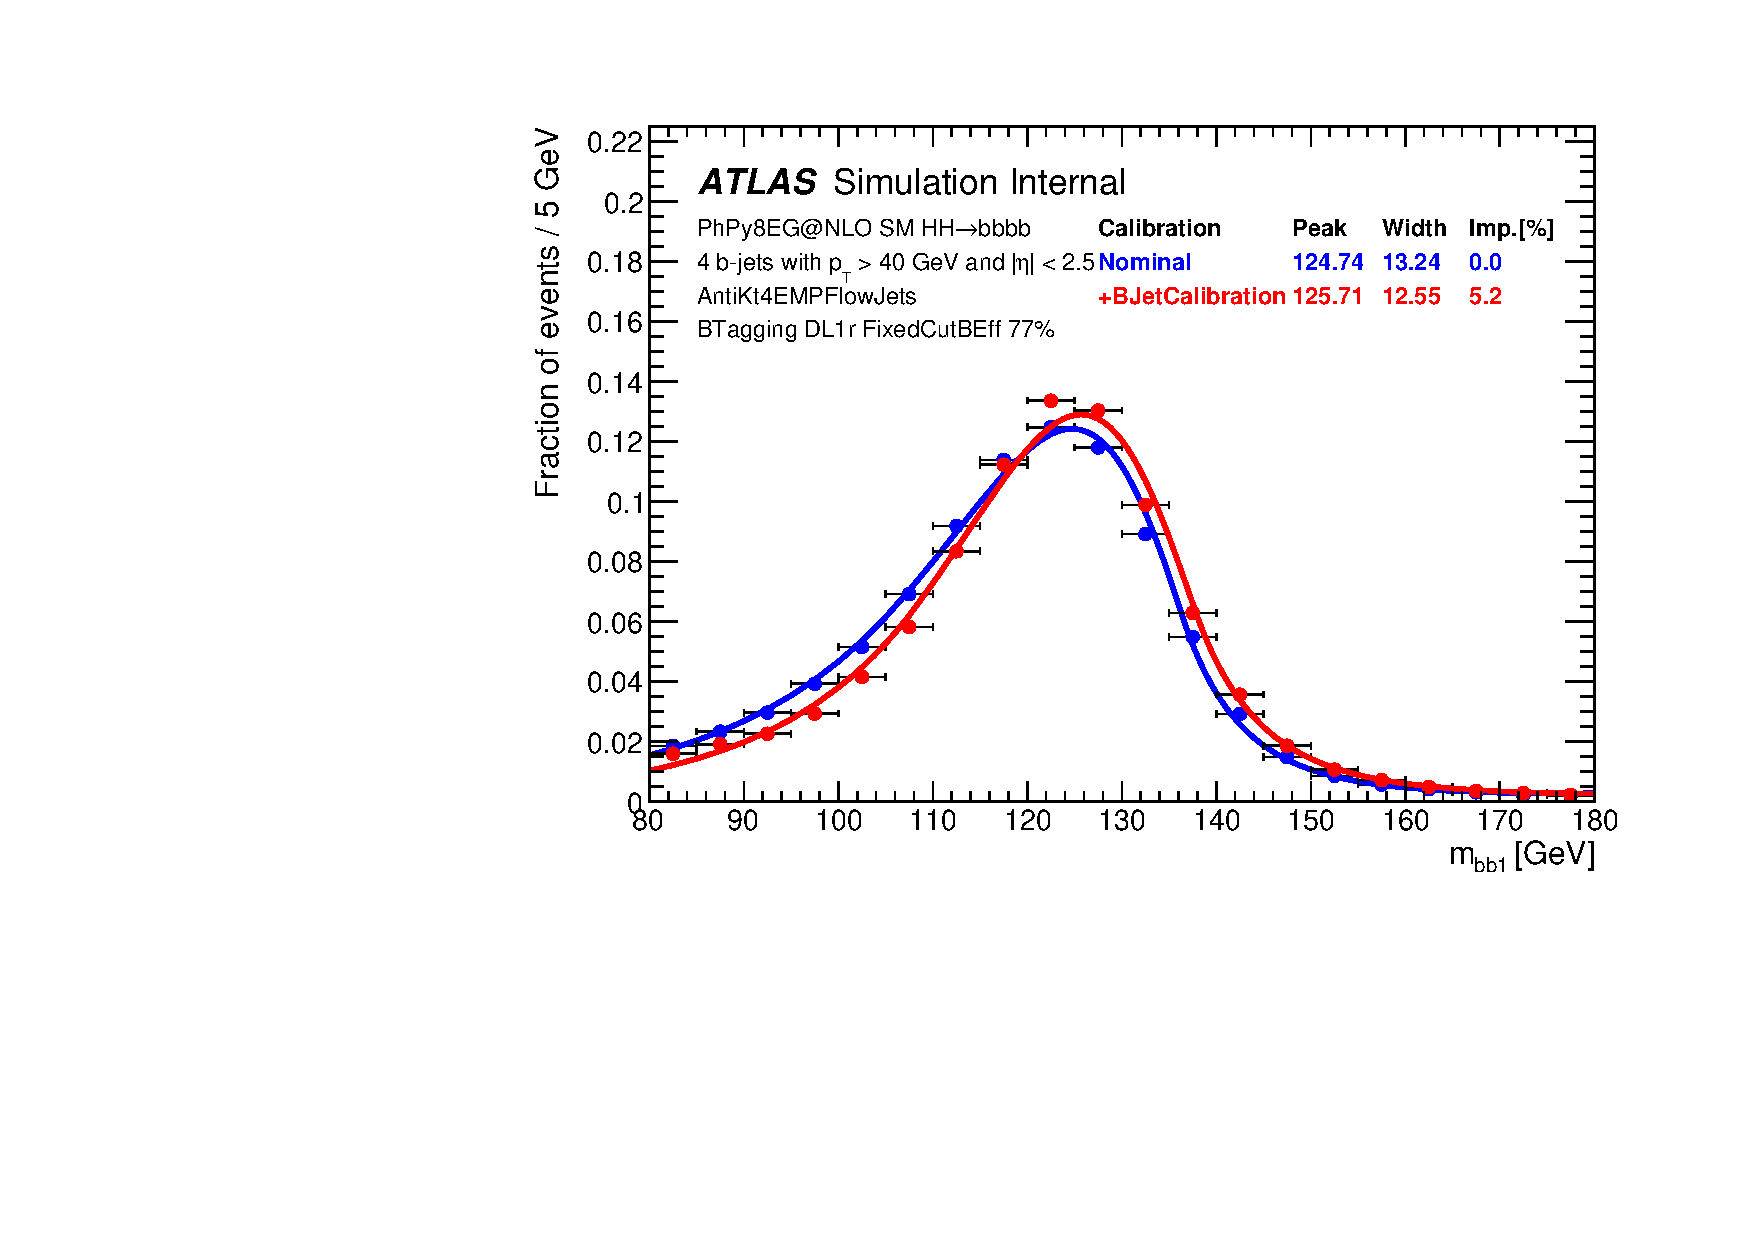
\includegraphics[width=0.33\textwidth]{\figpath/MAY21-Qs45-bjetcalib-Everything-18-m-h1-4b.pdf}
		\label{fig:bjetcalib-mh1}
	} 
	\subfloat[$m_{\PH2}$]{ 
	    	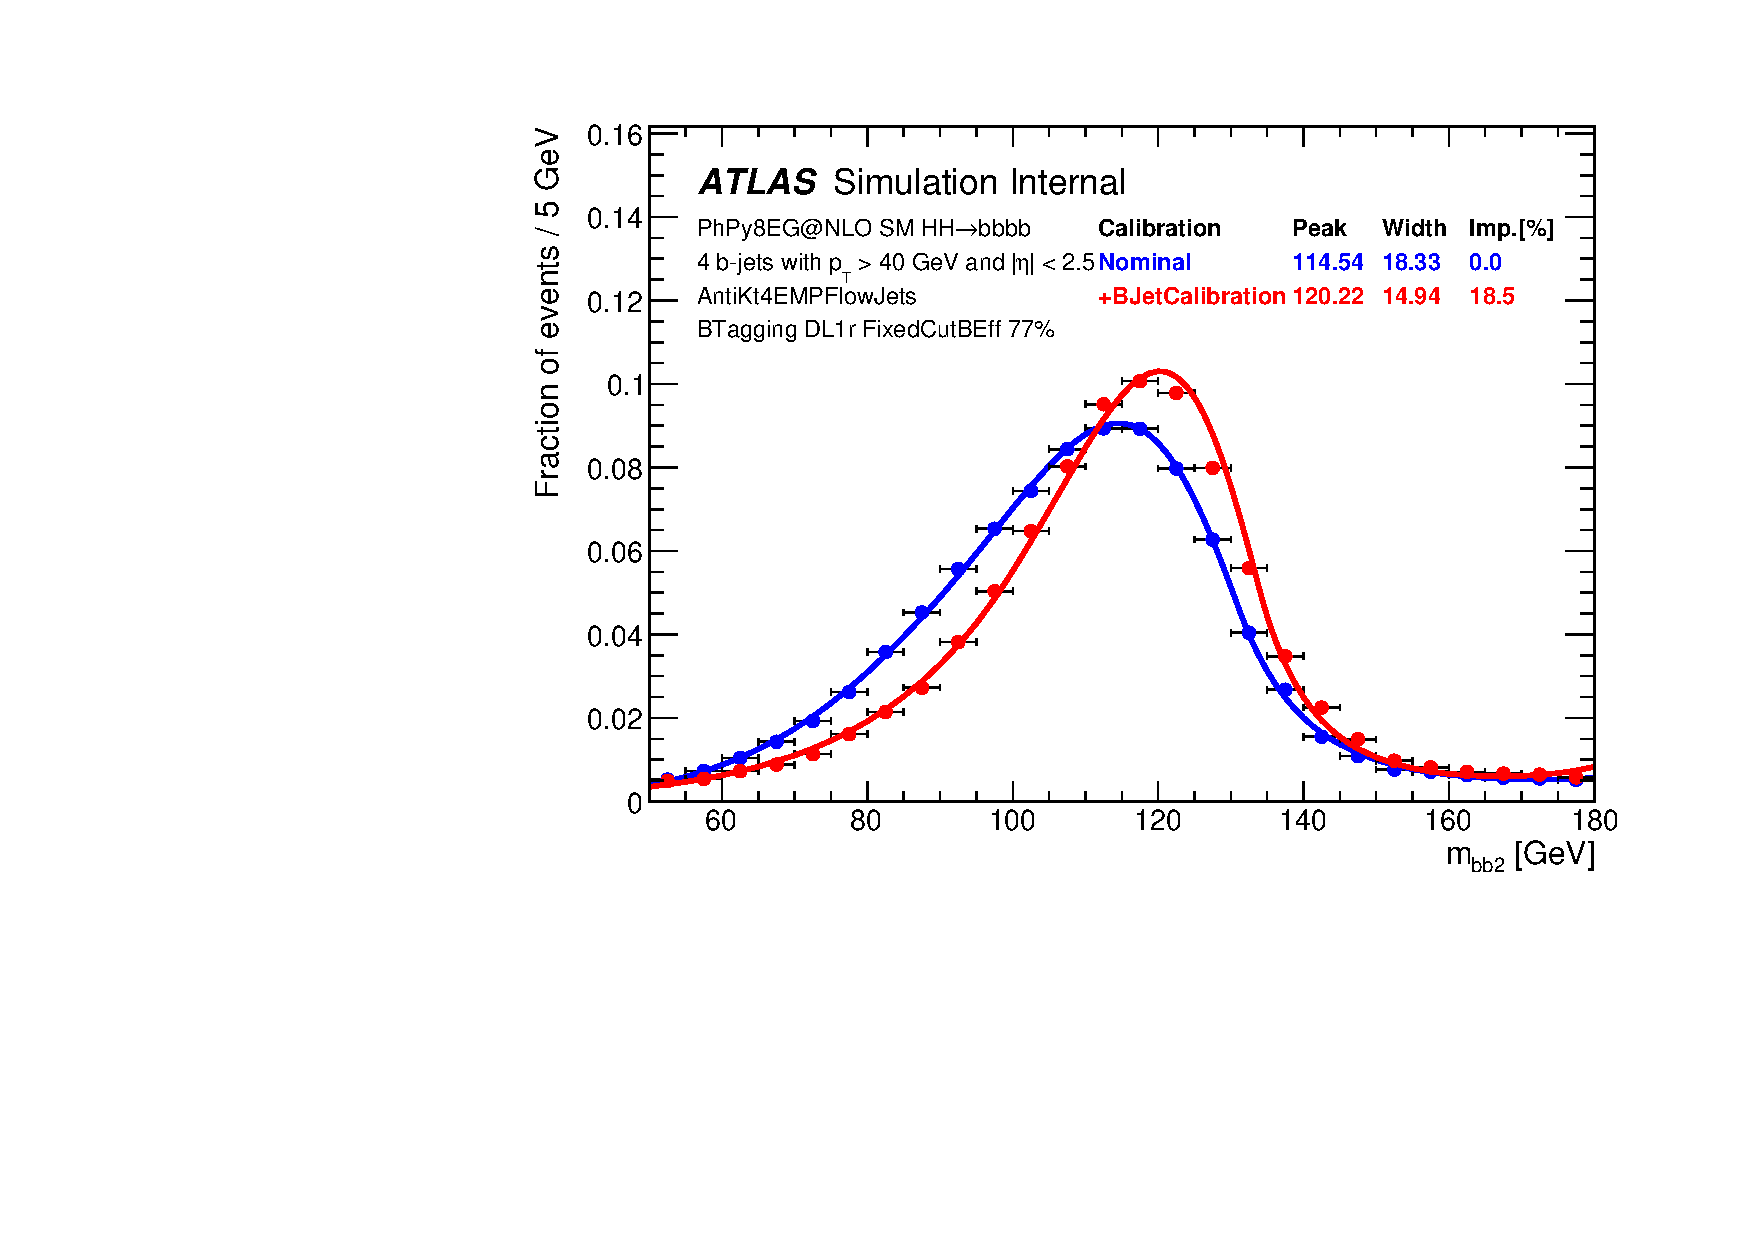
\includegraphics[width=0.33\textwidth]{\figpath/MAY21-Qs45-bjetcalib-Everything-18-m-h2-4b.pdf}
		\label{fig:bjetcalib-mh2}
	} 
	\subfloat[\mhh]{ 
	    	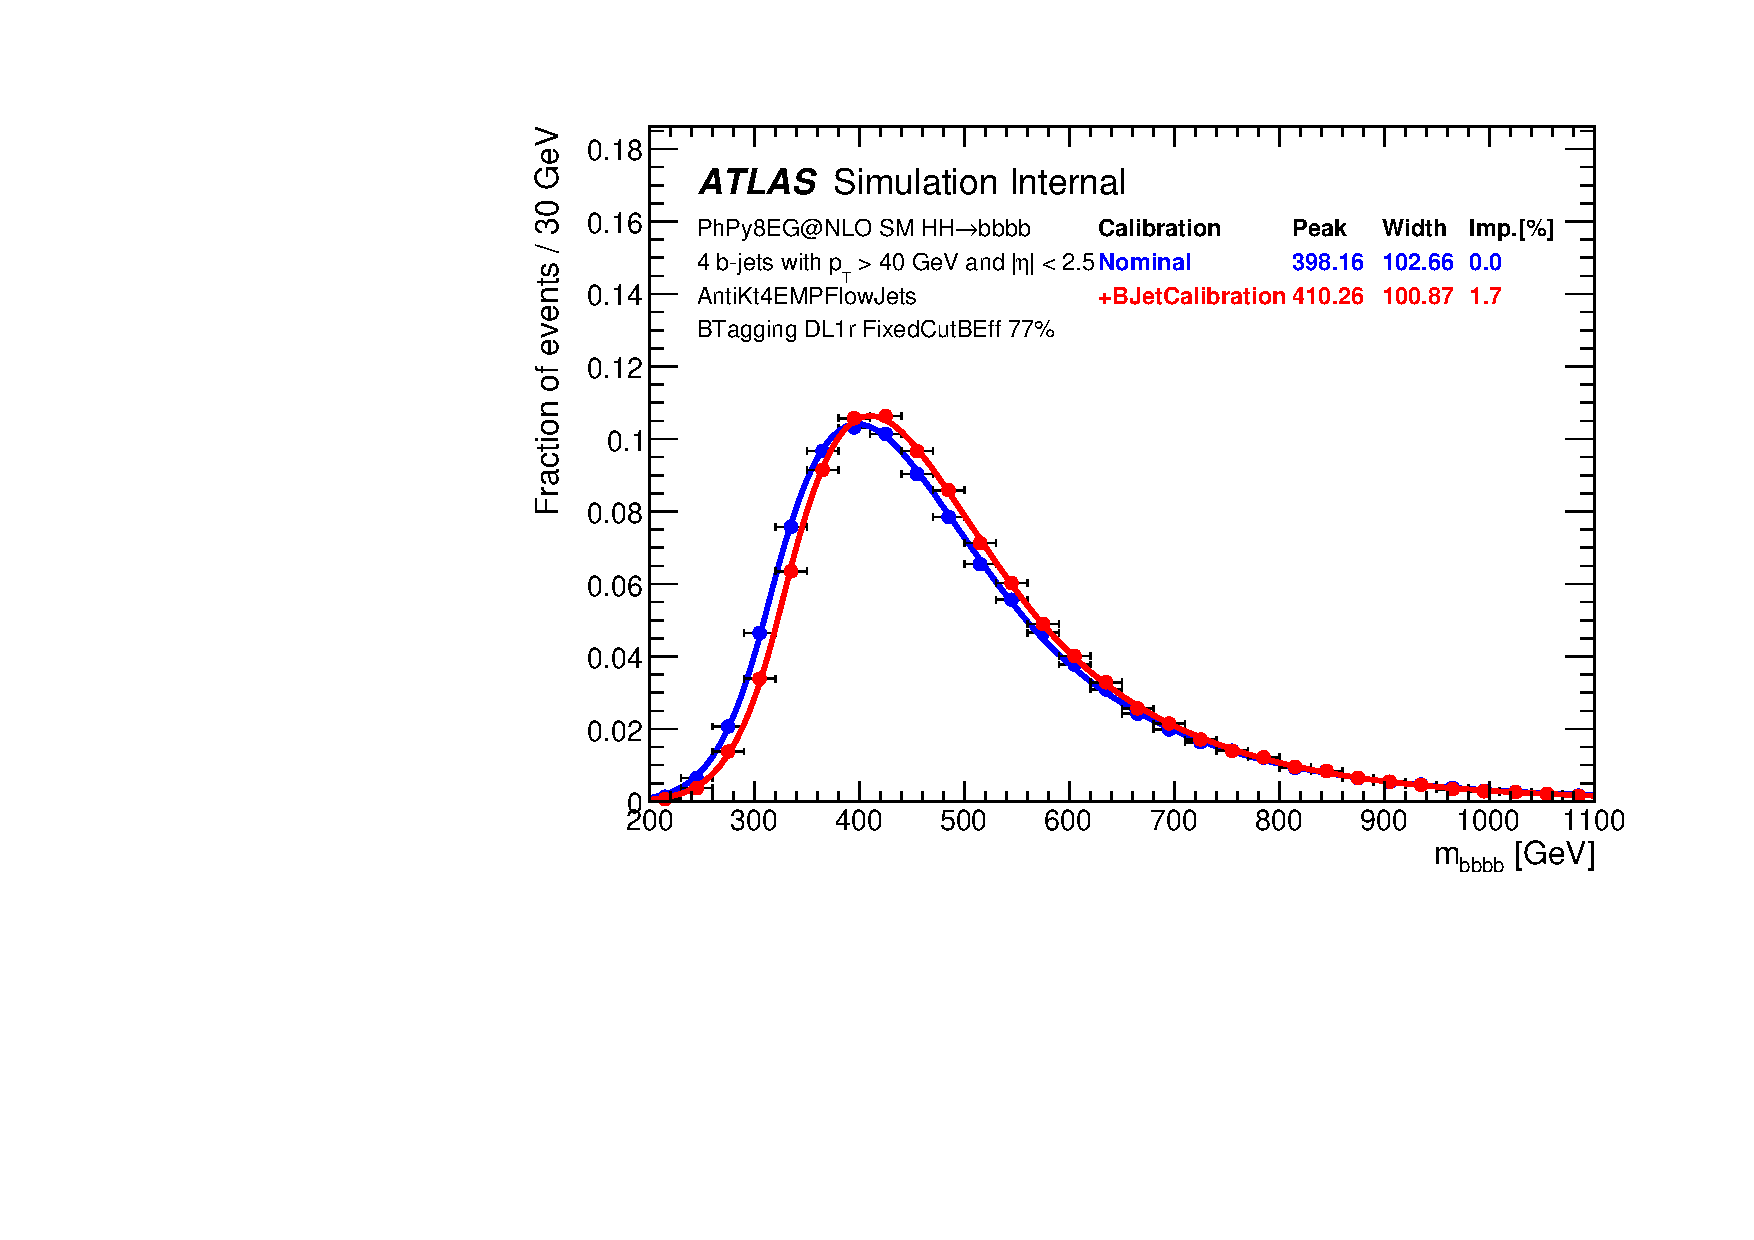
\includegraphics[width=0.33\textwidth]{\figpath/MAY21-Qs45-bjetcalib-Everything-18-m-hh-4b.pdf}
		\label{fig:bjetcalib-mhh}
	} 

	\caption{Comparisons of $m_{\PH1}$, $m_{\PH2}$ and \mhh distributions before the \Pqb-jet corrections~(blue) and 
                 after the \Pqb-jet corrections~(red). These distributions are fitted using Bukin function, and the peak, 
                 the peak resolusion and the relative improvement are shown in the legend.}
	\label{fig:bjetcalib-plots}
\end{figure}




\FloatBarrier
\clearpage

\section{Event selection}
\label{sec:event selection}

\subsection{Object Selection}

Jets are separated into two groups based on their kinematics: 
\begin{description}
	\item[\textit{Central} jets:] $|\eta| < 2.5,\ \pt \ge 40\ \GeV$ -  these jets are used for triggering and will form  Higgs-candidates;
	\item[\textit{Forward} jets:] $|\eta| \ge 2.5,\ \pt \ge 30\ \GeV$ - these extra jets are used to improve the acceptance of jets produced in the vector boson fusion production process.
\end{description}

\subsubsection{\Pqb-jets Selection}
\label{sec:sel-btag}

In order to maximize sensitivity, events are selected and categorized based on the number of \Pqb-tagged \textit{central} jets. 
The \Pqb-tagging algorithm used, DL1r, is described in \Sect{\ref{subsec:ftag}}. 

\paragraph{Ordering and selection} For the jets that form our Higgs Candidates, we take the four leading \Pqb-tagged jets. In events with less than four \Pqb-jets, the extra jets are selected as the highest $p_T$ jets from the pool of \textit{central} jets which failed the initial \Pqb-tag requirement.

\paragraph{\Pqb-tag Requirements} The \Pqb-tag selection for ggF and VBF signals is to require \textbf{at least 4 central jets with DL1r 77\% WP}. Events with two \bjets are classified as 2b events and are used for deriving the data-driven background estimate described in \Sect{\ref{sec:bkgdestimation}}. We also define a systematic on our background estimation using events with 3 \Pqb-tags, and the corresponding \Pqb-tag categories used in this analysis are summarized in table \ref{tab:b-tag-cat}.

\begin{table}[!htbp]
	\centering
	  \begin{tabularx}{\textwidth}{l|X|l}
	  Notation     & Definition & Usage \\
	  \toprule
	  2b    & Exactly two central jets tagged with DL1r 77\% WP & Background estimation \\ \hline
	  3b1f  & Exactly three central jets tagged with DL1r 77\% WP and no central jets passing the 85\% WP (the leading \pT non-\Pqb-jet is taken for the last Higgs Candidate jet) & Background estimate systematic \\ \hline
	  4b    & At least four central jets tagged with DL1r 77\% WP & Signal region (ggF and VBF) \\
	  \bottomrule
	  \end{tabularx}
	\caption{Different analysis definitions based on number of \Pqb-tags.}
	\label{tab:b-tag-cat}
  \end{table}%

  \paragraph{Accuracy} The Higgs jet selection accuracy is defined as the probability that all four \Pqb-jets in the event are matched to the truth \Pqb-quarks using a $\Delta R$ < 0.3 matching criterion, and is shown is \Fig{\ref{fig:jetSel-4b}}.
  The jet selection accuracy is 74\% for the ggF selection with \%-level variations across the \kl values of interest. 
  This means that there is a \SI{74}{\%} chance the selected four \Pqb-jets are coming from the real Higgs decayed \Pqb-quarks. This accuracy loss is dominated by events where one of the \Pqb-quarks is out of acceptance. 
  The 4b VBF selection has an average \Pqb-quark selection accuracy of 85\% and 90\% for the respective \kl and \kvv signal samples.
  The dependency on \kl and/or \kvv is likely due to the positive dependence of the \Pqb-tagging efficiency on the \Pqb-jet \pt: harder signals lead to higher \Pqb-tagging efficiency therefore higher Higgs jet selection accuracies. 
  \Fig{\ref{fig:jetSel-mhh}} shows the truth \mhh distributions and the reconstructed histograms for the cases where we did or did not selected the correct jets for the ggF and VBF selections at a few signal points. As discussed above, we are less likely to select the correct jets for lower \mhh, and also the signal shapes for the \kl and \kvv variations are quite different, this is entirely due to the underlying \mhh distribution.
    
  \begin{figure}[hbt]
	  \centering
	  \subfloat[Jet selection accuracy vs \kl]{
			   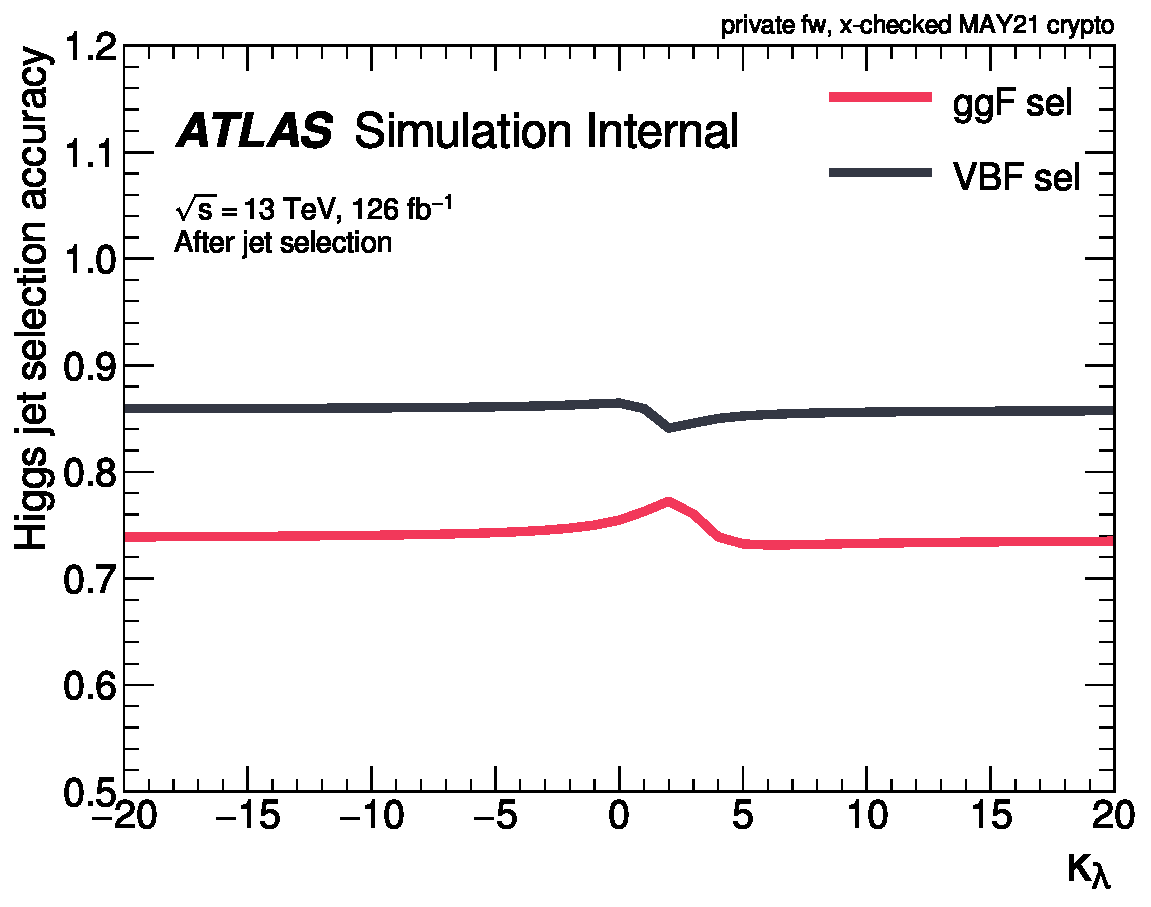
\includegraphics[width=0.4\textwidth]{figures/nr-int-note/selection/V2/jetSel_kl_4b_only.pdf}
		  \label{fig:jetSel-kl}
	  }
	  \subfloat[Jet selection accuracy vs $\kappa_{2V}$]{
			   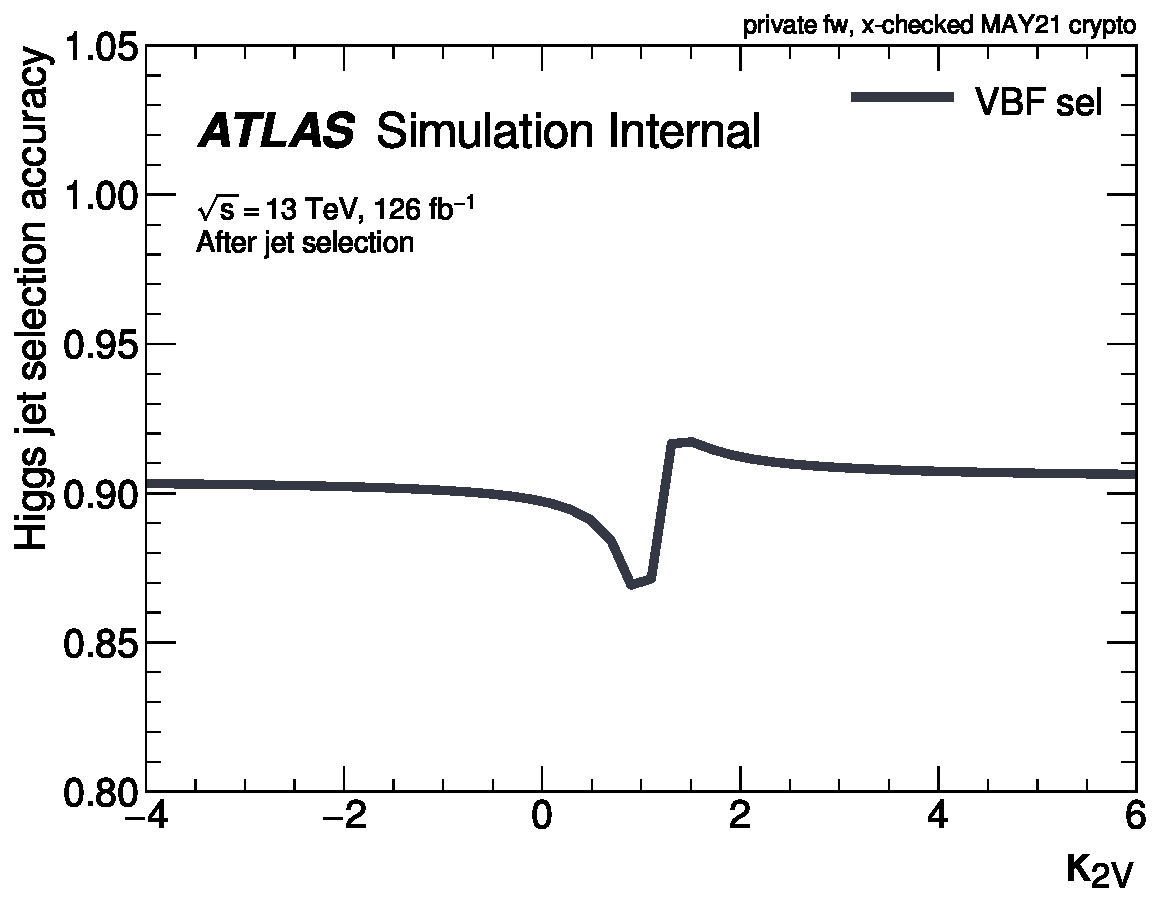
\includegraphics[width=0.4\textwidth]{figures/nr-int-note/selection/V2/jetSel_k2V.pdf} 
		  \label{fig:jetSel-k2V}
	  }
	  \caption{The jet selection accuracy as a function of \kl and \kvv.}
	  \label{fig:jetSel-4b}
  \end{figure}

  \begin{figure}[hbt]
	  \centering
	  \subfloat[ggF signals]{
			   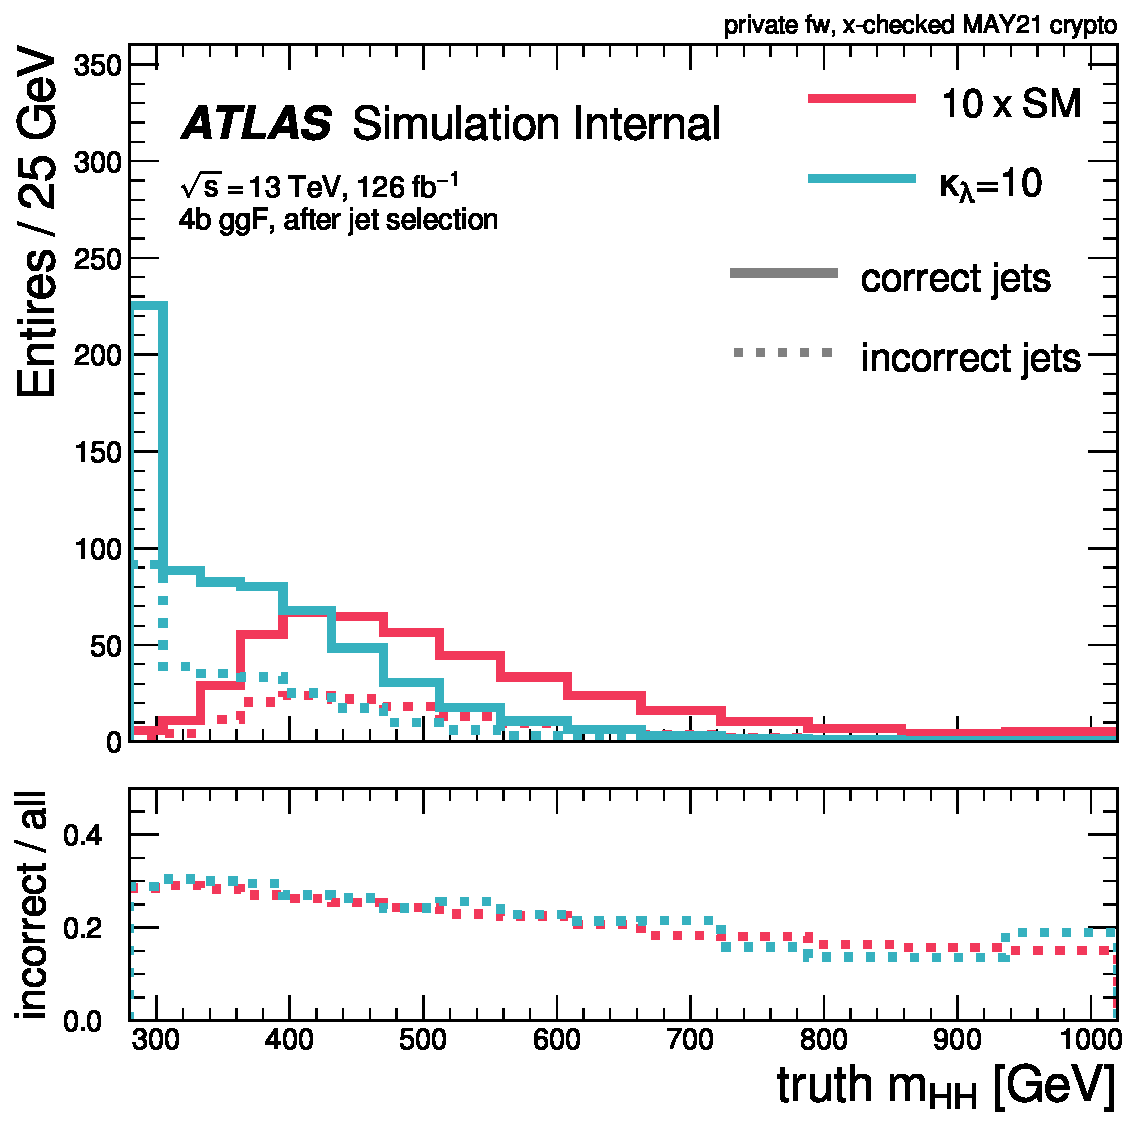
\includegraphics[width=0.4\textwidth]{figures/nr-int-note/selection/V2/truth_mhh_4b_jetSelAcc.pdf}
		  \label{fig:jetSel-kl}
	  }
	  \subfloat[VBF signals]{
			   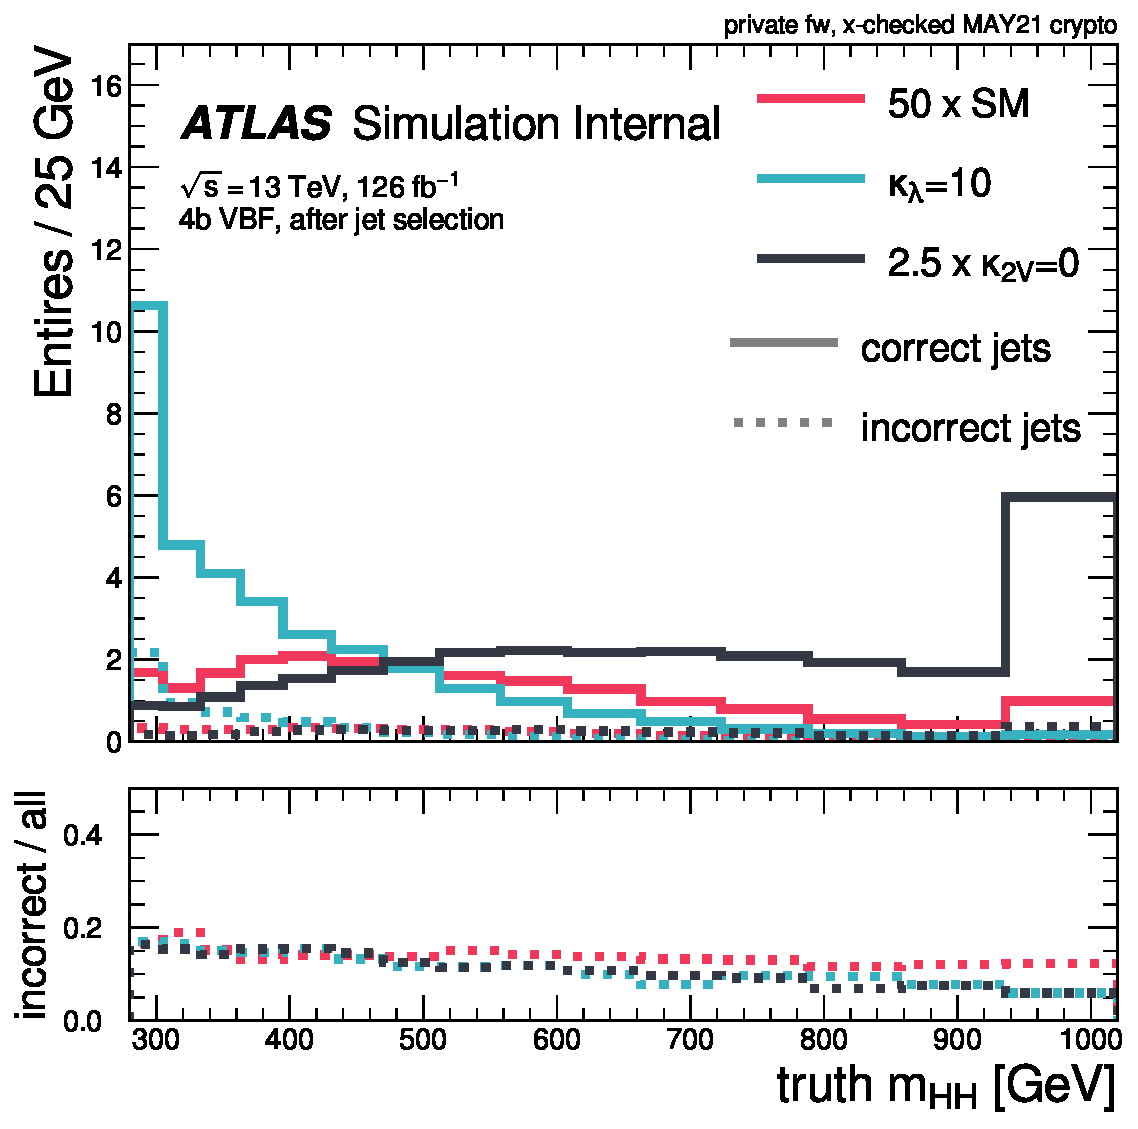
\includegraphics[width=0.4\textwidth]{figures/nr-int-note/selection/V2/truth_mhh_3b1l_jetSelAcc_vbf.pdf} 
		  \label{fig:jetSel-k2V}
	  }
	  \caption{Truth \mhh distributions for correctly and incorrectly selected jets, for ggF (a) and VBF (b) signals.}
	  \label{fig:jetSel-mhh}
  \end{figure}

\subsubsection{Definition of ggF and VBF Channels}

\hl{James wrote this... I need to rephrase}

This analysis possesses two channels targeting different \HH production processes. One is optimized for gluon-gluon fusion (ggF) and the other for vector boson fusion (VBF). The channel an event is placed in depends on whether it contains the two high energy and well-spaced jets characteristic of the VBF topology. If so, the event is placed in the VBF channel. If not, it is placed in the ggF channel. In this section, for ease of reading, these two jets will be referred to as the \textit{VBF Jets}.

First, to belong to the VBF channel, an event must possess a minimum of six jets. The VBF Jets are reconstructed as the two jets with the highest di-jet invariant mass ($m_{jj}$) from the pool of both central and forward jets that failed the b-tag requirement. If no such pair exists, the event is placed in the ggF channel.

To reduce the number of background events three cuts are then applied. If an event passes all three cuts it is placed in the VBF channel; otherwise, it is placed in the ggF channel. The first two are a cut on the rapidity-gap between the VBF Jets of $\detajj > 3$ and on their combined invariant mass of $m_{jj} > 1000\ \GeV$. Finally, the six four-vectors corresponding to the \HH and VBF Jets are summed, and a requirement applied that the \pt of that combined four-vector be less than 65 \GeV. The \HH is not reconstructed until after events are placed into VBF and ggF channels. Here, the same method for identifying the \HH jets as in the reconstruction is used only to facilitate applying this cut.

If an event passes the VBF channel criteria, the jets used to reconstruct the VBF jets are removed from the pool of jets that the \HH can be reconstructed from.

The ggF and VBF channels are designed to be orthogonal in order to facilitate statistically combining them when deriving results. 
As shown in \Sect{\ref{subsec:sigYields}} \Tab{\ref{tab:ggF_4SR_yields}}, a negligible fraction of ggF signal is leaked in the VBF channel even with the priority of the VBF selection. %; while the cuts applied to the VBF Jets were optimized for the VBF signal. 
When optimizing the analysis, we saw the impact of the VBF veto for our ggF signals was at the 2\% level, and as such, this deemed orthogonalization strategy to be acceptable.

\subsubsection{Higgs candidate pairing}
\label{subsubsec:higgs-pairing}

The \HH system is reconstructed from two \textit{Higgs candidates}, which are themselves reconstructed from two jets each (four \textit{Higgs candidate jets} in total). These jets are selected from the pool of central jets. \bjets are selected first. If the event is a 4b event, the leading four in \pt are selected. If it is a 2b event, the remaining places are filled by non-b-tagged jets, which are sorted in \pt and the two leading jets taken. For details on the \Pqb-tag based selection, see \Sect{\ref{sec:sel-btag}}.

We define \textbf{pairing} as the identification of a jet pair as a Higgs candidate. Given the four selected \textit{Higgs candidate jets}, three possible pairings are possible, as sketched in Figure \ref{fig:poss-pairs}. We must therefore devise a strategy that accurately predicts which pairing is correct. 
The \textbf{correct pairing} is defined with generator level information. First, \Pqb-quarks are matched to \Pqb-jets using a $\Delta R < 0.3$ criterion. The correct pair is then defined by the \Pqb-quarks which have the same parent barcode ID in the truth record.

The pairing method chosen in this iteration of the analysis is based on the principle that the decay products of the Higgs should show a degree of collimation due to the Higgs's initial momentum. Of the two Higgs boson candidates in a given pairing, the \textit{leading} Higgs candidate is defined as the one with the highest \pt. For each of the three pairing options, the leading Higgs candidate is identified and the $\Delta R_{Leading}(jj)$ between its two constituent jets calculated. 
The pairing option with the smallest $\Delta R_{Leading}(jj)$ is selected.
% The leading Higgs candidate associated with the smallest $\Delta R$ is selected. The remaining two jets are then taken as the other Higgs candidate.

\begin{figure}[b]
    \centering
    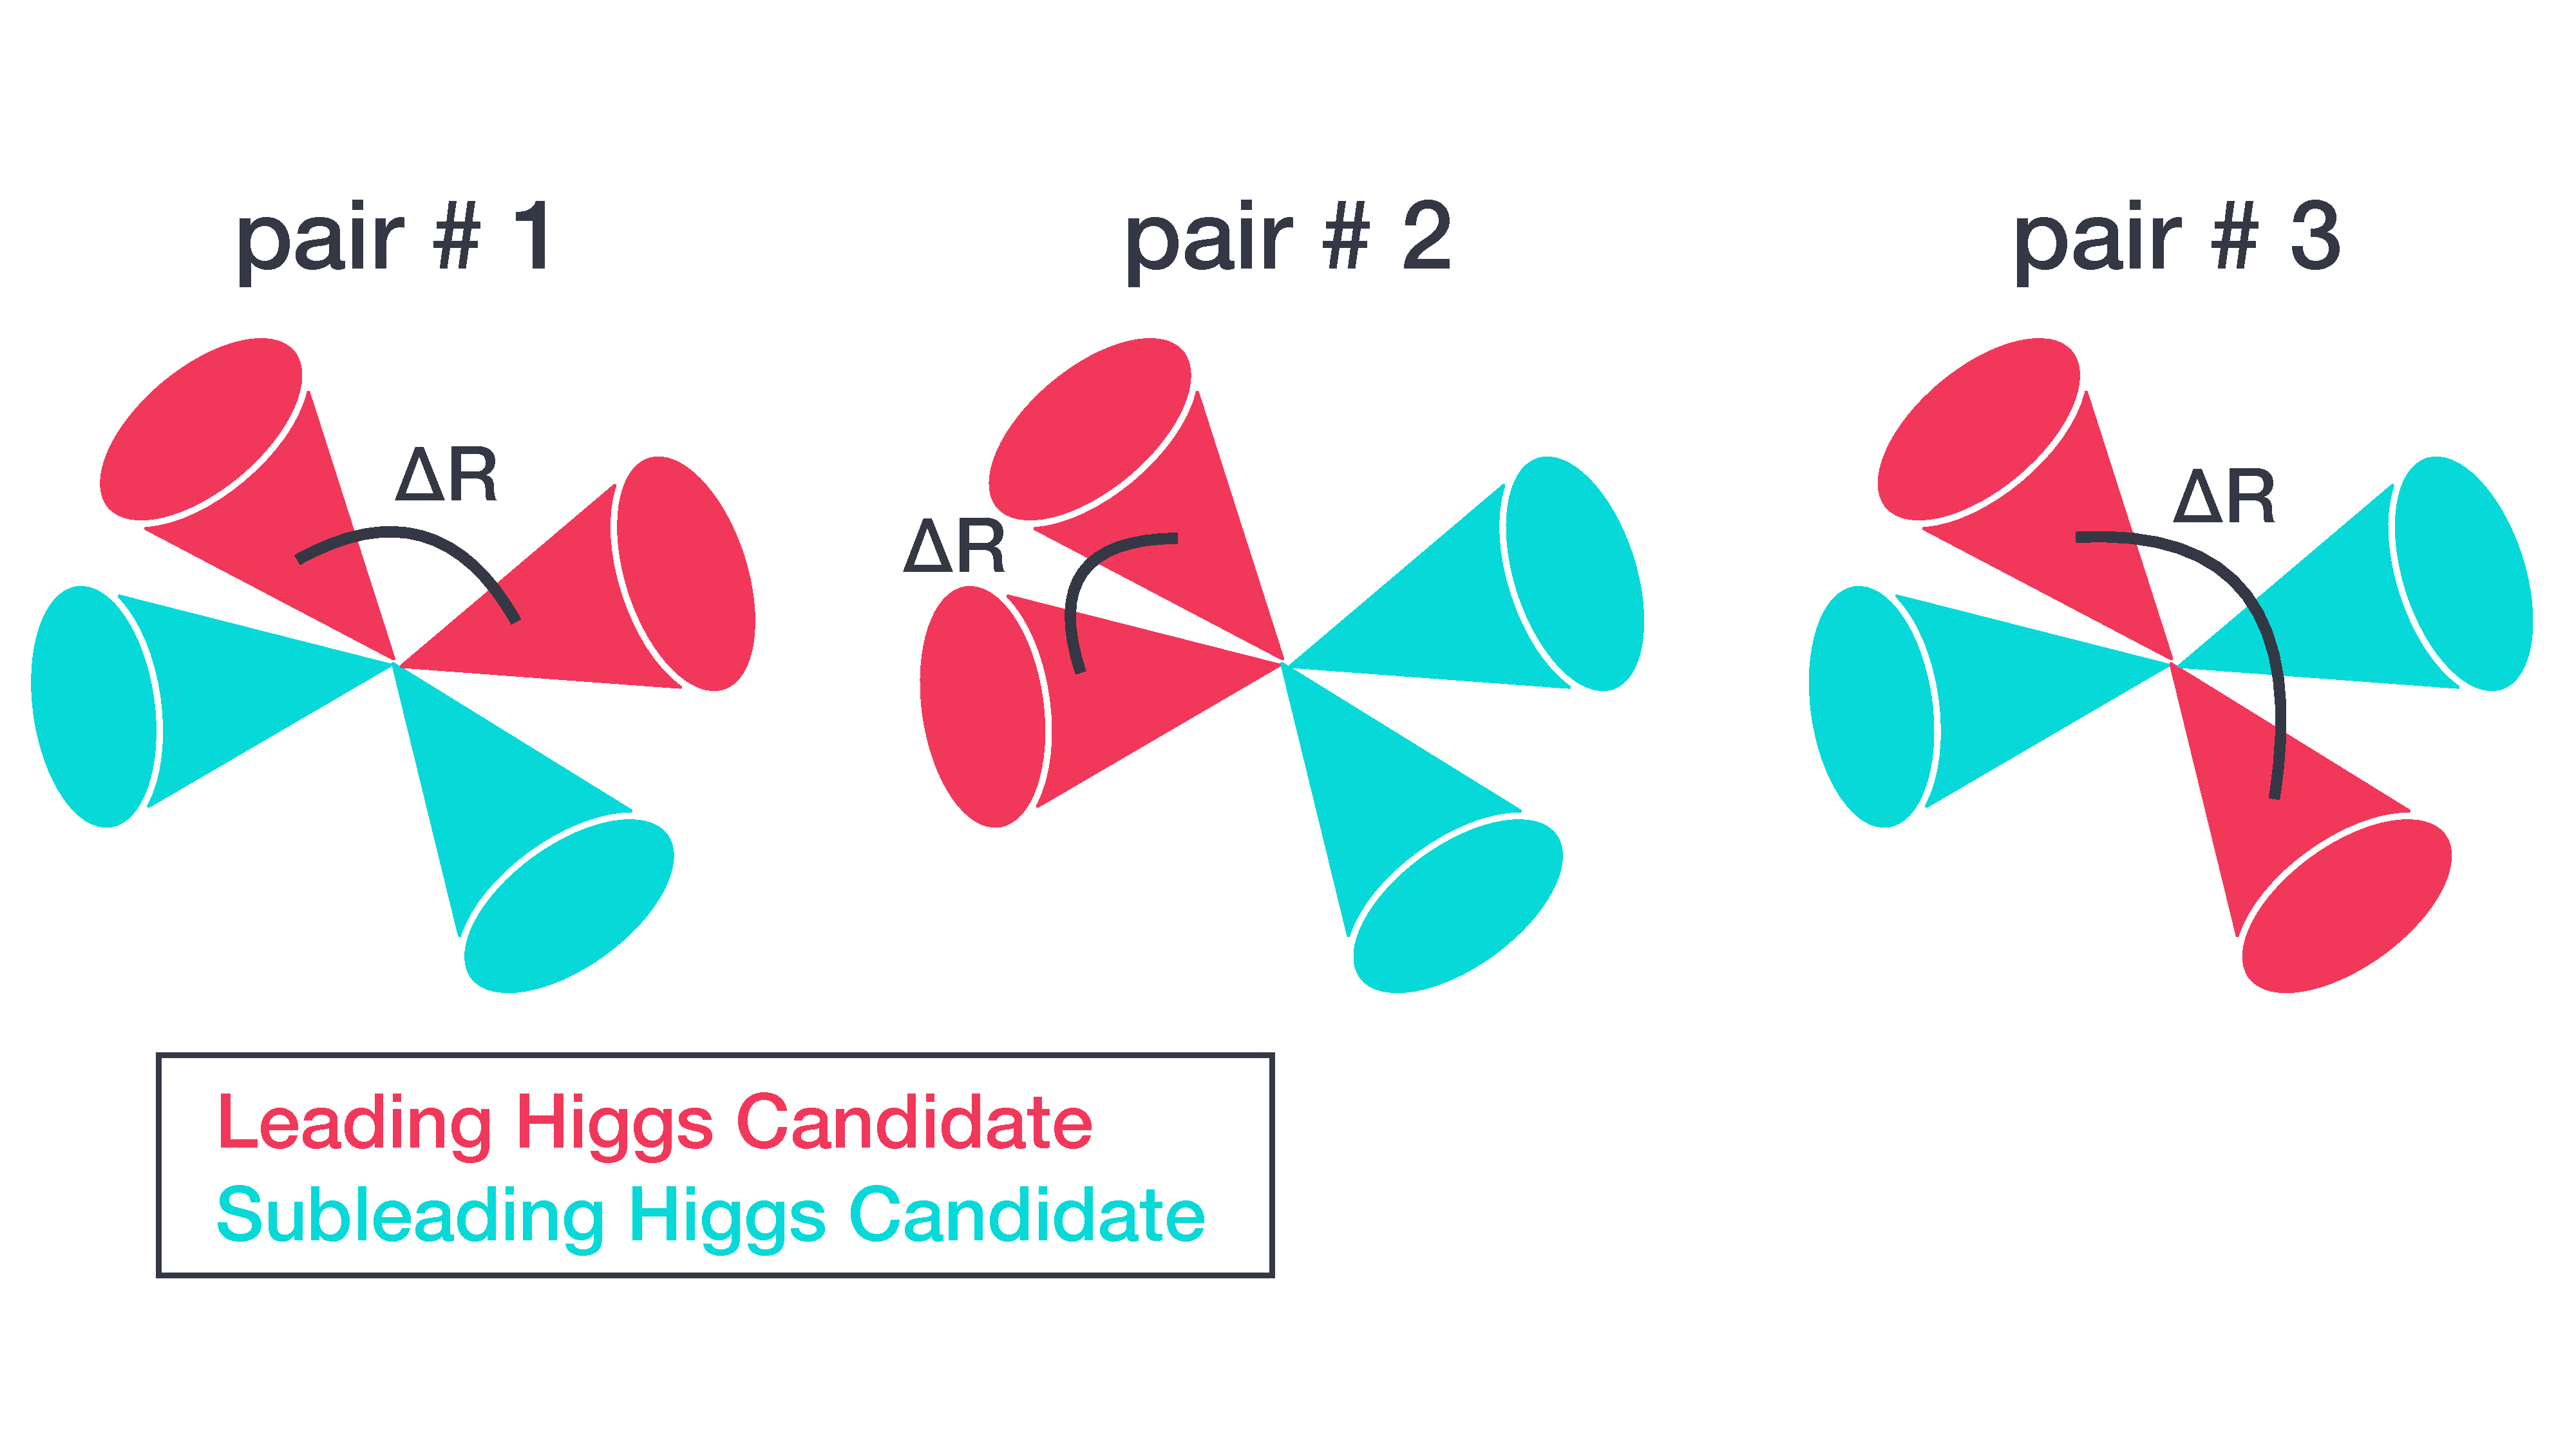
\includegraphics[width=0.8\textwidth,,trim=0 4cm 0 5cm,clip]{figures/nr-int-note/selection/V2/pairing.pdf}
    \caption{The three possible pairing permutations of the four \HH jets into the two Higgs candidates.  The opening angles between the jets in the leading Higgs Candidate are indicated, so pair number 2 is the selected pairing.}
    \label{fig:poss-pairs}
\end{figure}

\paragraph{Pairing accuracy} The pairing accuracy is defined as the fraction of correctly paired events among the events where the four Higgs-decayed jets are corrected selected by the jet selection. This definition is selected to decouple the pairing accuracy from the jet selection accuracy, as defined in \Sect{\ref{sec:sel-btag}}. The pairing accuracy is shown in \Fig{\ref{fig:pairingAcc-exists-4b}} as a function of \kl and \kvv, and in \Fig{\ref{fig:pairingAcc-mhh-exists-4b}} as a function of \mhh.
Signals with harder \pt Higgs tend to have more collimated jet pairs, resulting in higher pairing accuracies. 
This effect leads to a loss of accuracy for low $m_{HH}$ events (i.e., $m_{HH} < 450$ GeV), as also seen a drop of the pairing accuracy with non-SM \kl values or SM-like \kvv values as they lead to softer kinematics. This is deemed acceptable because most of the analysis background is also located at low $m_{HH}$, therefore losing these events do not reflect in a loss of performance.


\begin{figure}[hbt]
	\centering
	\subfloat[Pairing accuracy vs \kl]{
	     	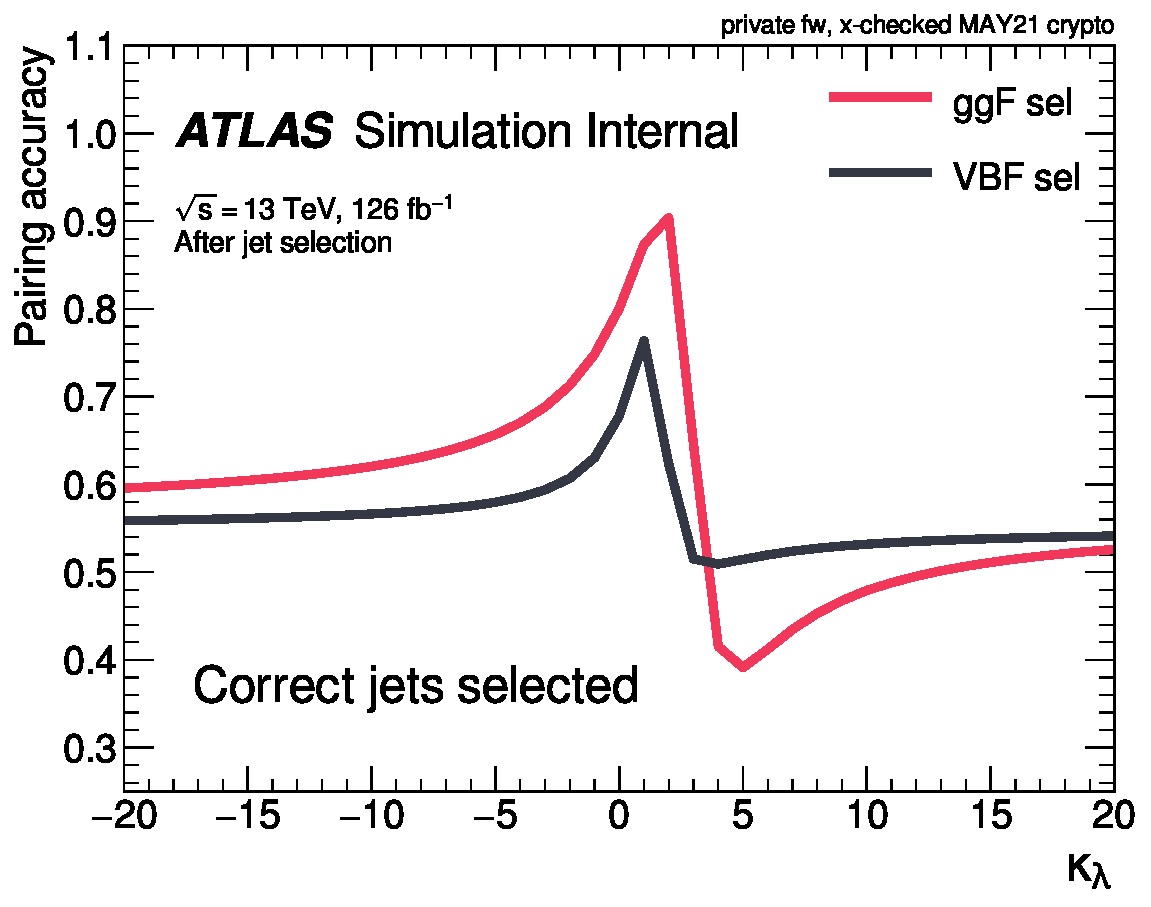
\includegraphics[width=0.4\textwidth]{figures/nr-int-note/selection/V2/acc_kl_exists_4b_only.pdf}
		\label{fig:pairingAcc-kl-exists-4b}
	}
	\subfloat[Pairing accuracy vs $\kappa_{2V}$]{
	     	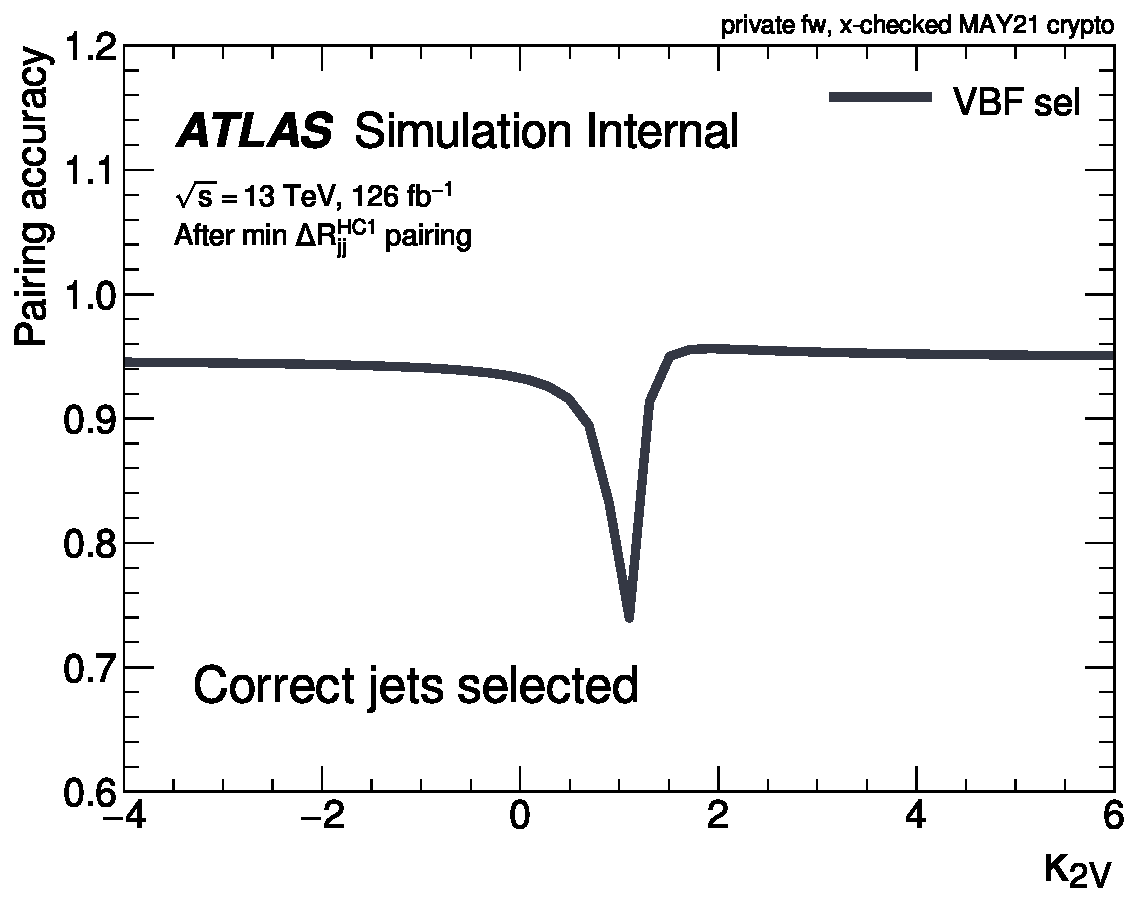
\includegraphics[width=0.4\textwidth]{figures/nr-int-note/selection/V2/acc_k2V_exists.pdf} 
		\label{fig:pairingAcc-k2V-exists}
	}
	\caption{The pairing accuracy as a function of \kl and \kvv, given that the correct jets have been selected.}
	\label{fig:pairingAcc-exists-4b}
\end{figure}

\begin{figure}[b]
    \centering
    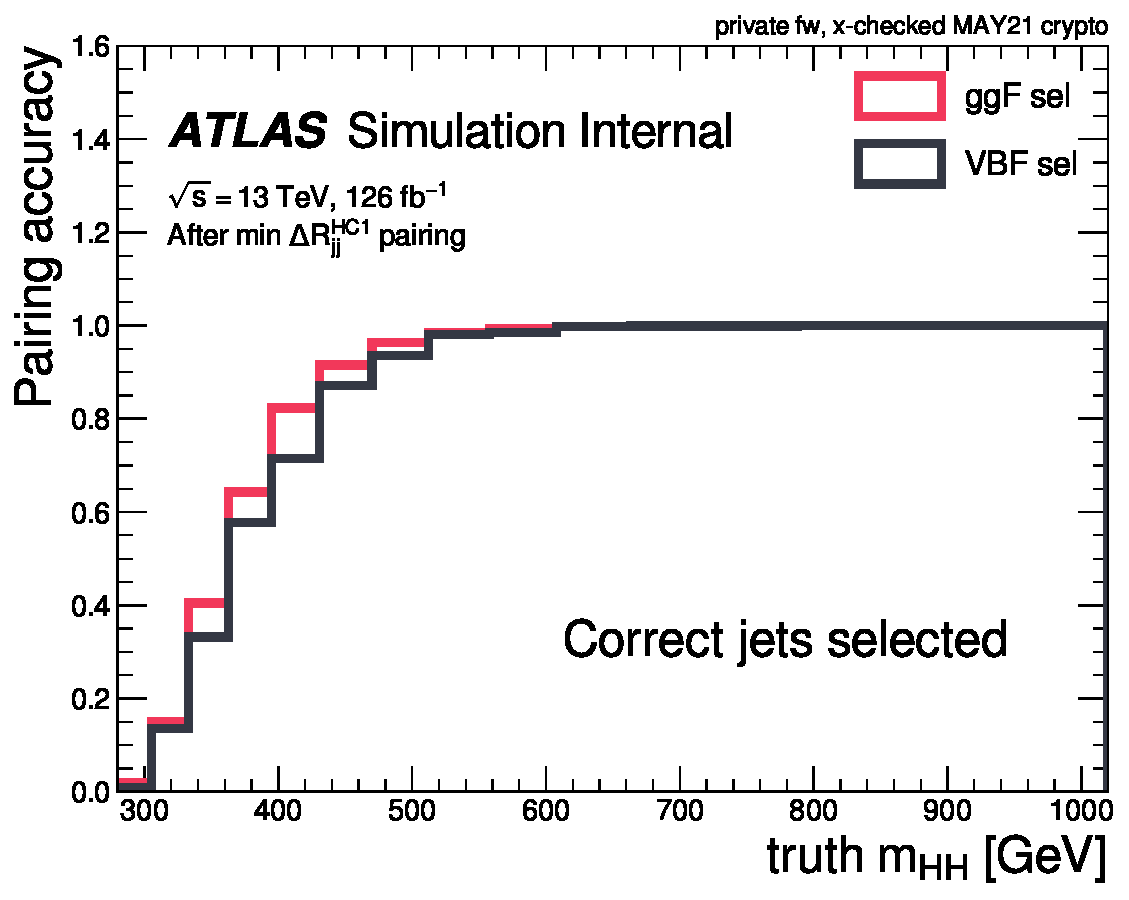
\includegraphics[width=0.5\textwidth]{figures/nr-int-note/selection/V2/acc_truth_mhh_exists_4b_only.pdf}
    \caption{Pairing accuracy as a function of truth \mhh, given that the correct jets have been selected. The ggF selection accuracy is derived from the ggF SM sample, and the VBF selection accuracy is derived from the VBF \kvv sample.}
    \label{fig:pairingAcc-mhh-exists-4b}
\end{figure}

\FloatBarrier



\subsection{Background Reduction and \ttbar Veto}
\label{subsec:bkg-reduction}

\hl{Rui wrote this - I need to rephrase!}

In order to suppress background, a pseudorapidity separation of $\deta < 1.5$ is required between the two Higgs candidates in the ggF channel. This cut is not used in the VBF channel as it reduces sensitivity to SM VBF \HH production. \Fig{\ref{fig:dEta-ggf}} shows the \deta distributions for ggF \HH signal and blinded data\footnote{By blinded data, we mean we do not show data events that fall in our 4b signal region as defined by \Eqn{\ref{eq:xhh}}.} in the ggF channel immediately after the pairing. It demonstrates that the data in the $(m_{H1}, m_{H2})$ plane, which is a good approximation of the background, tends to have higher values than those of the signal. Therefore, such a cut is applied to improve the signal purity.
It is worth mentioning that a cut on the Higgs candidate \pt was applied in the previous publication, but was found to not be as powerful in the recent resonant search~\cite{pT_Cut_and_Muon-in-jet_Correction}.
Therefore, it is dropped in this analysis.

\begin{figure}[b]
    \centering
    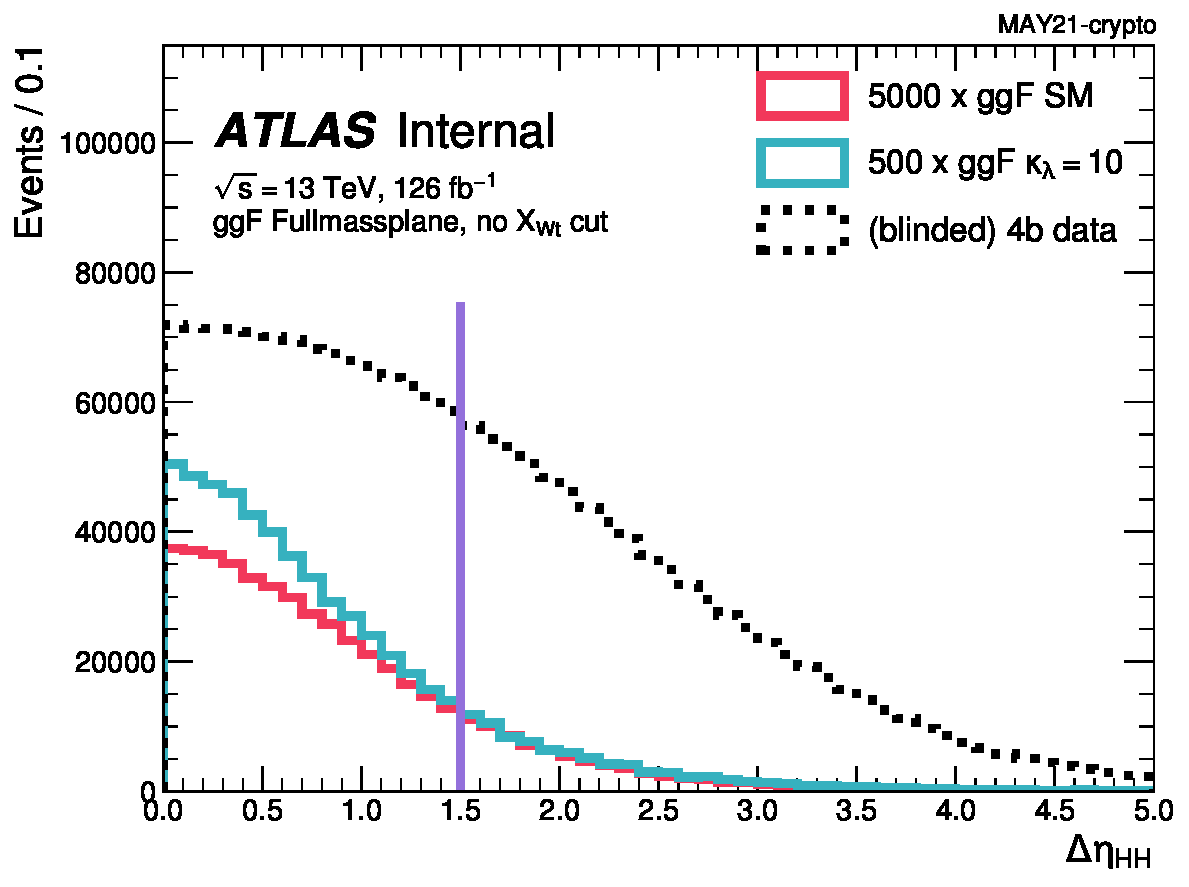
\includegraphics[width=0.5\textwidth]{figures/nr-int-note/selection/V3/dEta_hh_ggF_fullmassplane_all_4b_sm_k10.pdf}
    \caption{The \deta distribution for SM ggF \HH Monte Carlo simulation and blinded data in the ggF channel. The solid purple line indicates the \deta < 1.5 cut that is applied in the ggF selection. Events to the right of this line are discarded.}
    \label{fig:dEta-ggf}
\end{figure}

Additionally, a top veto is applied to suppress the background from hadronic top-quark decays.
This is applied by cutting on a discriminant, $\Xwt$, that is constructed to measure the compatibility of an event to contain a hadronically decaying top-quark.
To construct $\Xwt$, \PW candidates are formed from any pair of jets with $\pt > \SI{40}{\GeV}$ and $|\eta| < 2.5$, including those that were not selected for the Higgs candidates or for the VBF jets.
All possible \PW candidates are considered, and top candidates are built by pairing \PW candidates with any remaining \Pqb-jets that were selected for Higgs candidates.
The discriminant $\Xwt$ is constructed for each combination, expressed as:
\begin{equation}
    \Xwt = \sqrt{\left(\frac{m_{\PW} - \SI{80.4}{\GeV}}{0.1 \ m_{\PW}}\right)^{2} + \left(\frac{m_{\Pqt} - \SI{172.5}{\GeV}}{0.1 \ m_{\Pqt}}\right)^{2}}
    \label{eqn:xwt}
\end{equation}
Events are then vetoed if the minimum $\Xwt$ over all combinations is less than \num{1.5}.
\Fig{\ref{fig:Xwt}} shows the effectiveness of this cut at reducing the $t\bar{t}$ background while keeping a high efficiency for our signals.

\begin{figure}[ht]
	\centering
	\subfloat[4b ggF selection]{ %  with the ggF selection
	    	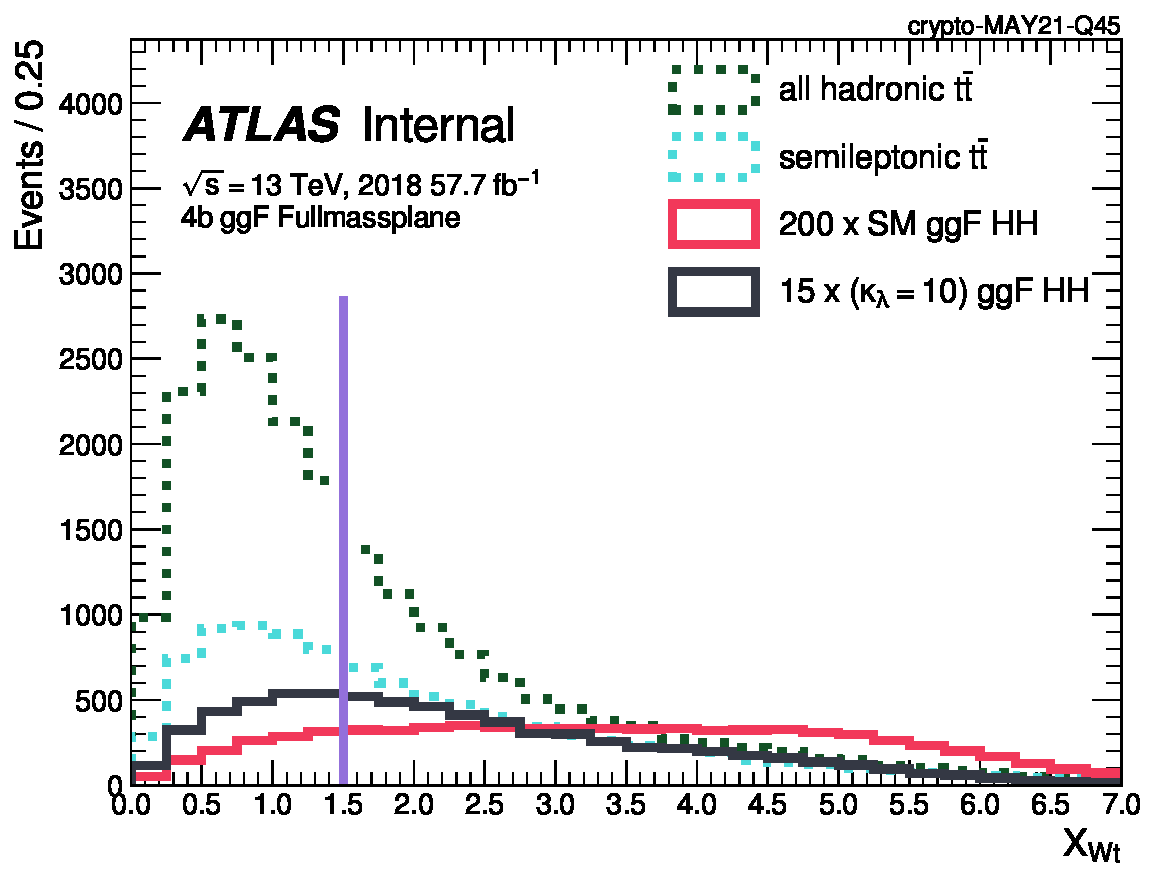
\includegraphics[width=0.44\textwidth]{figures/nr-int-note/selection/V4/X_wt_tag-ggf-4b-18}
		\label{fig:Xwt-ggf-4b}
	}
	\subfloat[4b VBF selection]{ % with the VBF selection
	    	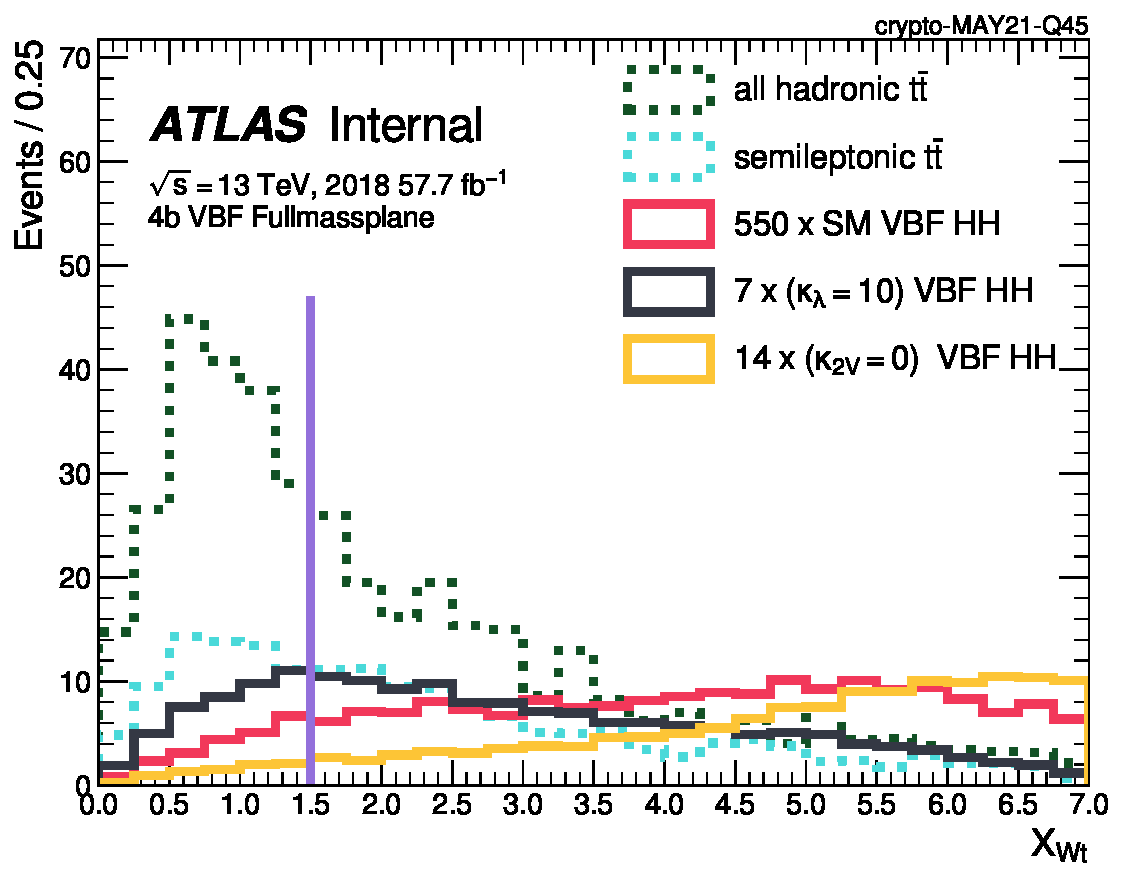
\includegraphics[width=0.44\textwidth]{figures/nr-int-note/selection/V4/X_wt_tag-vbf-4b-18}
 		\label{fig:Xwt-ggf-4b}
	}
	\caption{\Xwt distributions for our analysis categories in the 2018 dataset.
	The solid pink line indicates the $\Xwt$ > 1.5 cut applied to both the ggF and VBF channels.
	Event on the left of the line are discarded.}
	\label{fig:Xwt}
\end{figure}


We require the jet from Higgs candidates that is paired with the \PW candidate to be \textbf{\Pqb-tagged} while in the previous analyses there is no such a requirement.
%Although this requirement does not have any impact on the 4b events, it impacts 2b events, lowering the uncertainties on the background estimate\footnote{\href{https://indico.cern.ch/event/994939/contributions/4182687/}{https://indico.cern.ch/event/994939/contributions/4182687/}}.
% If I want to say this, I think I'll need to include the plots


\subsection{Kinematic Region Definition}
\label{sec:selection:region}

The final cut defining our signal region uses \Xhh as given by \Eqn{\ref{eq:xhh}}. The functional form of this variable is similar to the equation for an ellipse, except that the radius is a function of the Higgs Candidate (HC) masses to allow harsher cuts for higher HC masses where the jets' resolution is better. This is easiest to see by looking at the SR shape in one of the mass planes, i.e, the purple line in \Fig{\ref{fig:ggF-massplanes-allYrs-SM}}, since the "egg shaped" SR has allows for more acceptance at lower HC masses.

\begin{equation}
    \Xhh =  \sqrt{\left(\frac{m_{\PH1} - \SI{124}{\GeV}}{0.1 \ m_{\PH1}}\right)^{2} + \left(\frac{m_{\PH2} - \SI{117}{\GeV}}{0.1 \ m_{\PH2}}\right)^{2}} .
    \label{eq:xhh}
\end{equation}

The values (124, 117) in the \Xhh definition were chosen to approximately match the centers of the $m_{H1}$ and $m_{H2}$ distributions for correctly paired signal events. 
The signal region (SR) is defined in \Eqn{\ref{eq:sr}}, as visualized in the solid pink line in the $(m_{H1}, m_{H2})$ signal mass plane in \Fig{\ref{fig:massplanes-allYrs-signal}}. For both the ggF SM signal and the VBF $\kappa_{2V} = 0$, these signal events are nicely peaking inside of this SR, and for the softer $\kappa_\lambda$ = 10 spectrum are shown in \Fig{\ref{fig:massplanes-allYrs-kl-10}} of \App{\ref{app:evt-sel}}.
\Fig{\ref{fig:ggF-Xhh}} shows \Xhh for correctly and incorrectly paired signal (SM for the ggF selection and $\kappa_{2V} = 0$ for the VBF selection), and demonstrates that this SR defining cut value of 1.6 has a high purity of correctly paired signal events.
The SR center is re-optimized w.r.t.\ the 4b resonant analysis~\cite{bbbbresolvedNote}, where (120, 110) is used, as the kinematics and mass coverage of both analyses are different.
Alternative SR were also tested including a standard ellipse or larger size~\cite{slides:SR-opt}.
No improvement in the background modeling was observed with the alternatives.

\begin{figure}[ht]
	\centering
	\subfloat[4b ggF SM signal]{ %  with the ggF selection
	    	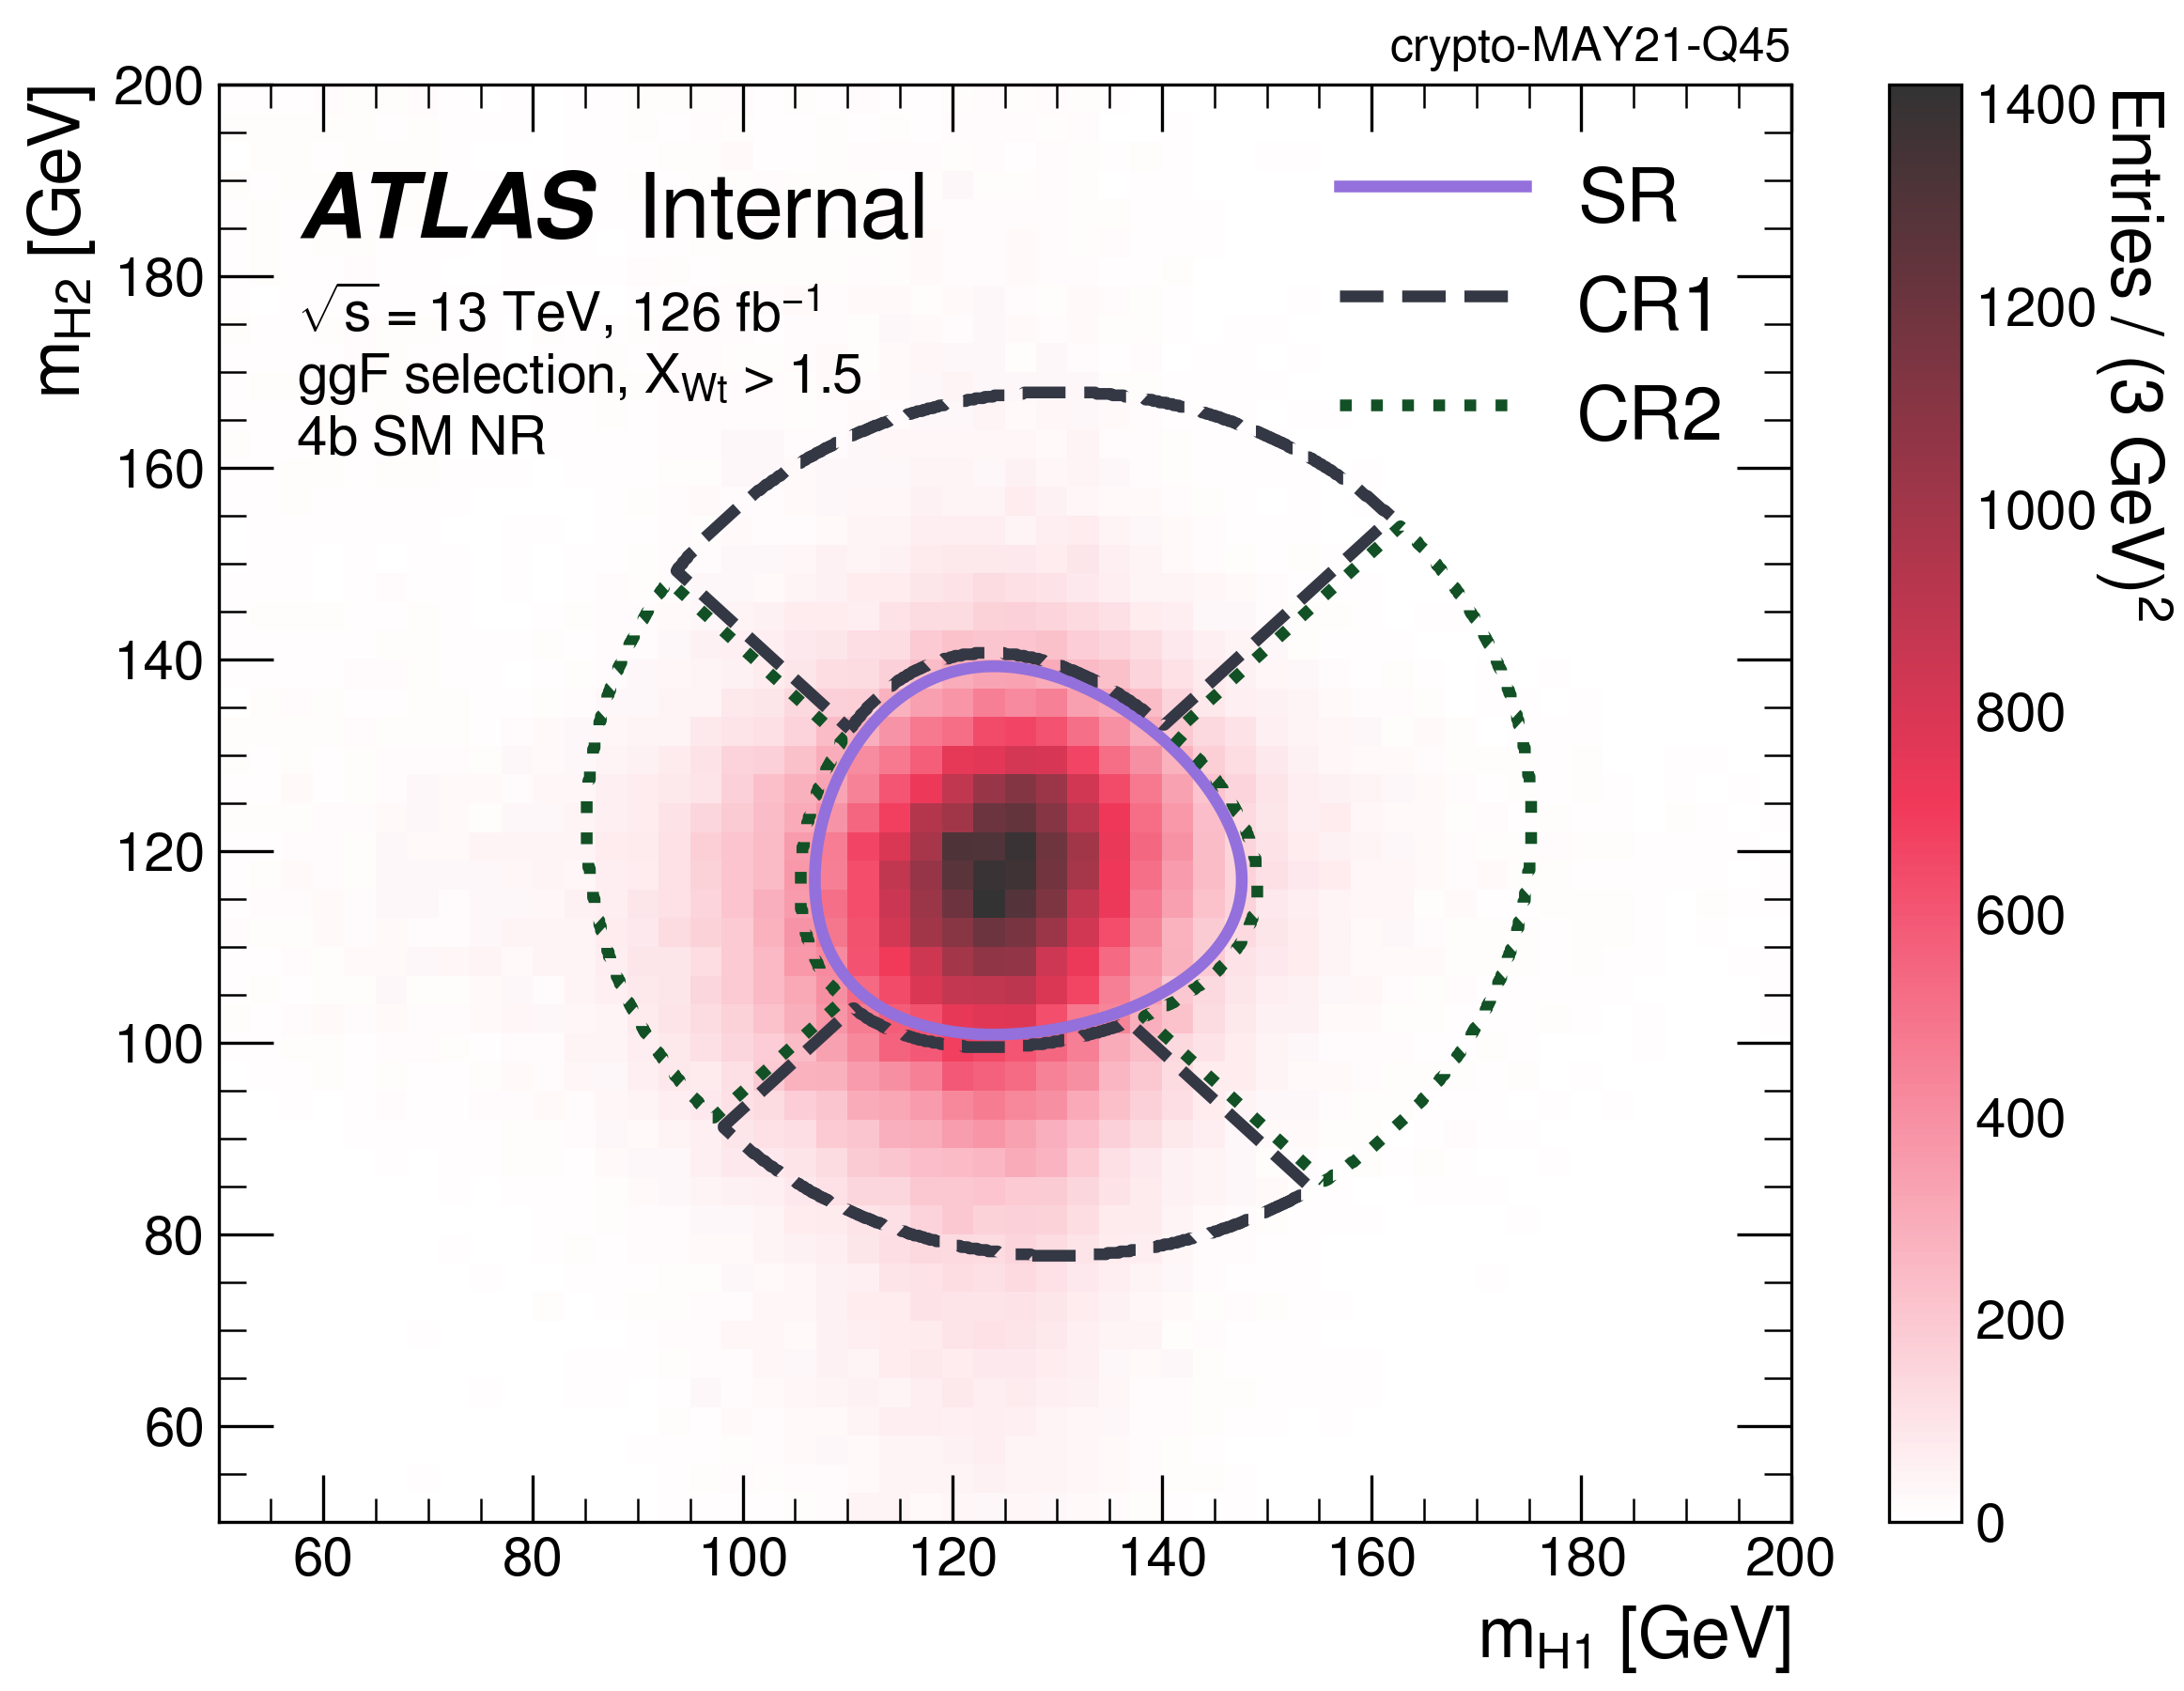
\includegraphics[width=0.4\textwidth]{figures/nr-int-note/selection/V3/massplane_sig_all_4b_ggf_Xwt_1.5.png}
		\label{fig:ggF-massplanes-allYrs-SM}
	}
	\subfloat[4b $\kappa_{2V} = 0$ signal]{ % with the VBF selection
	    	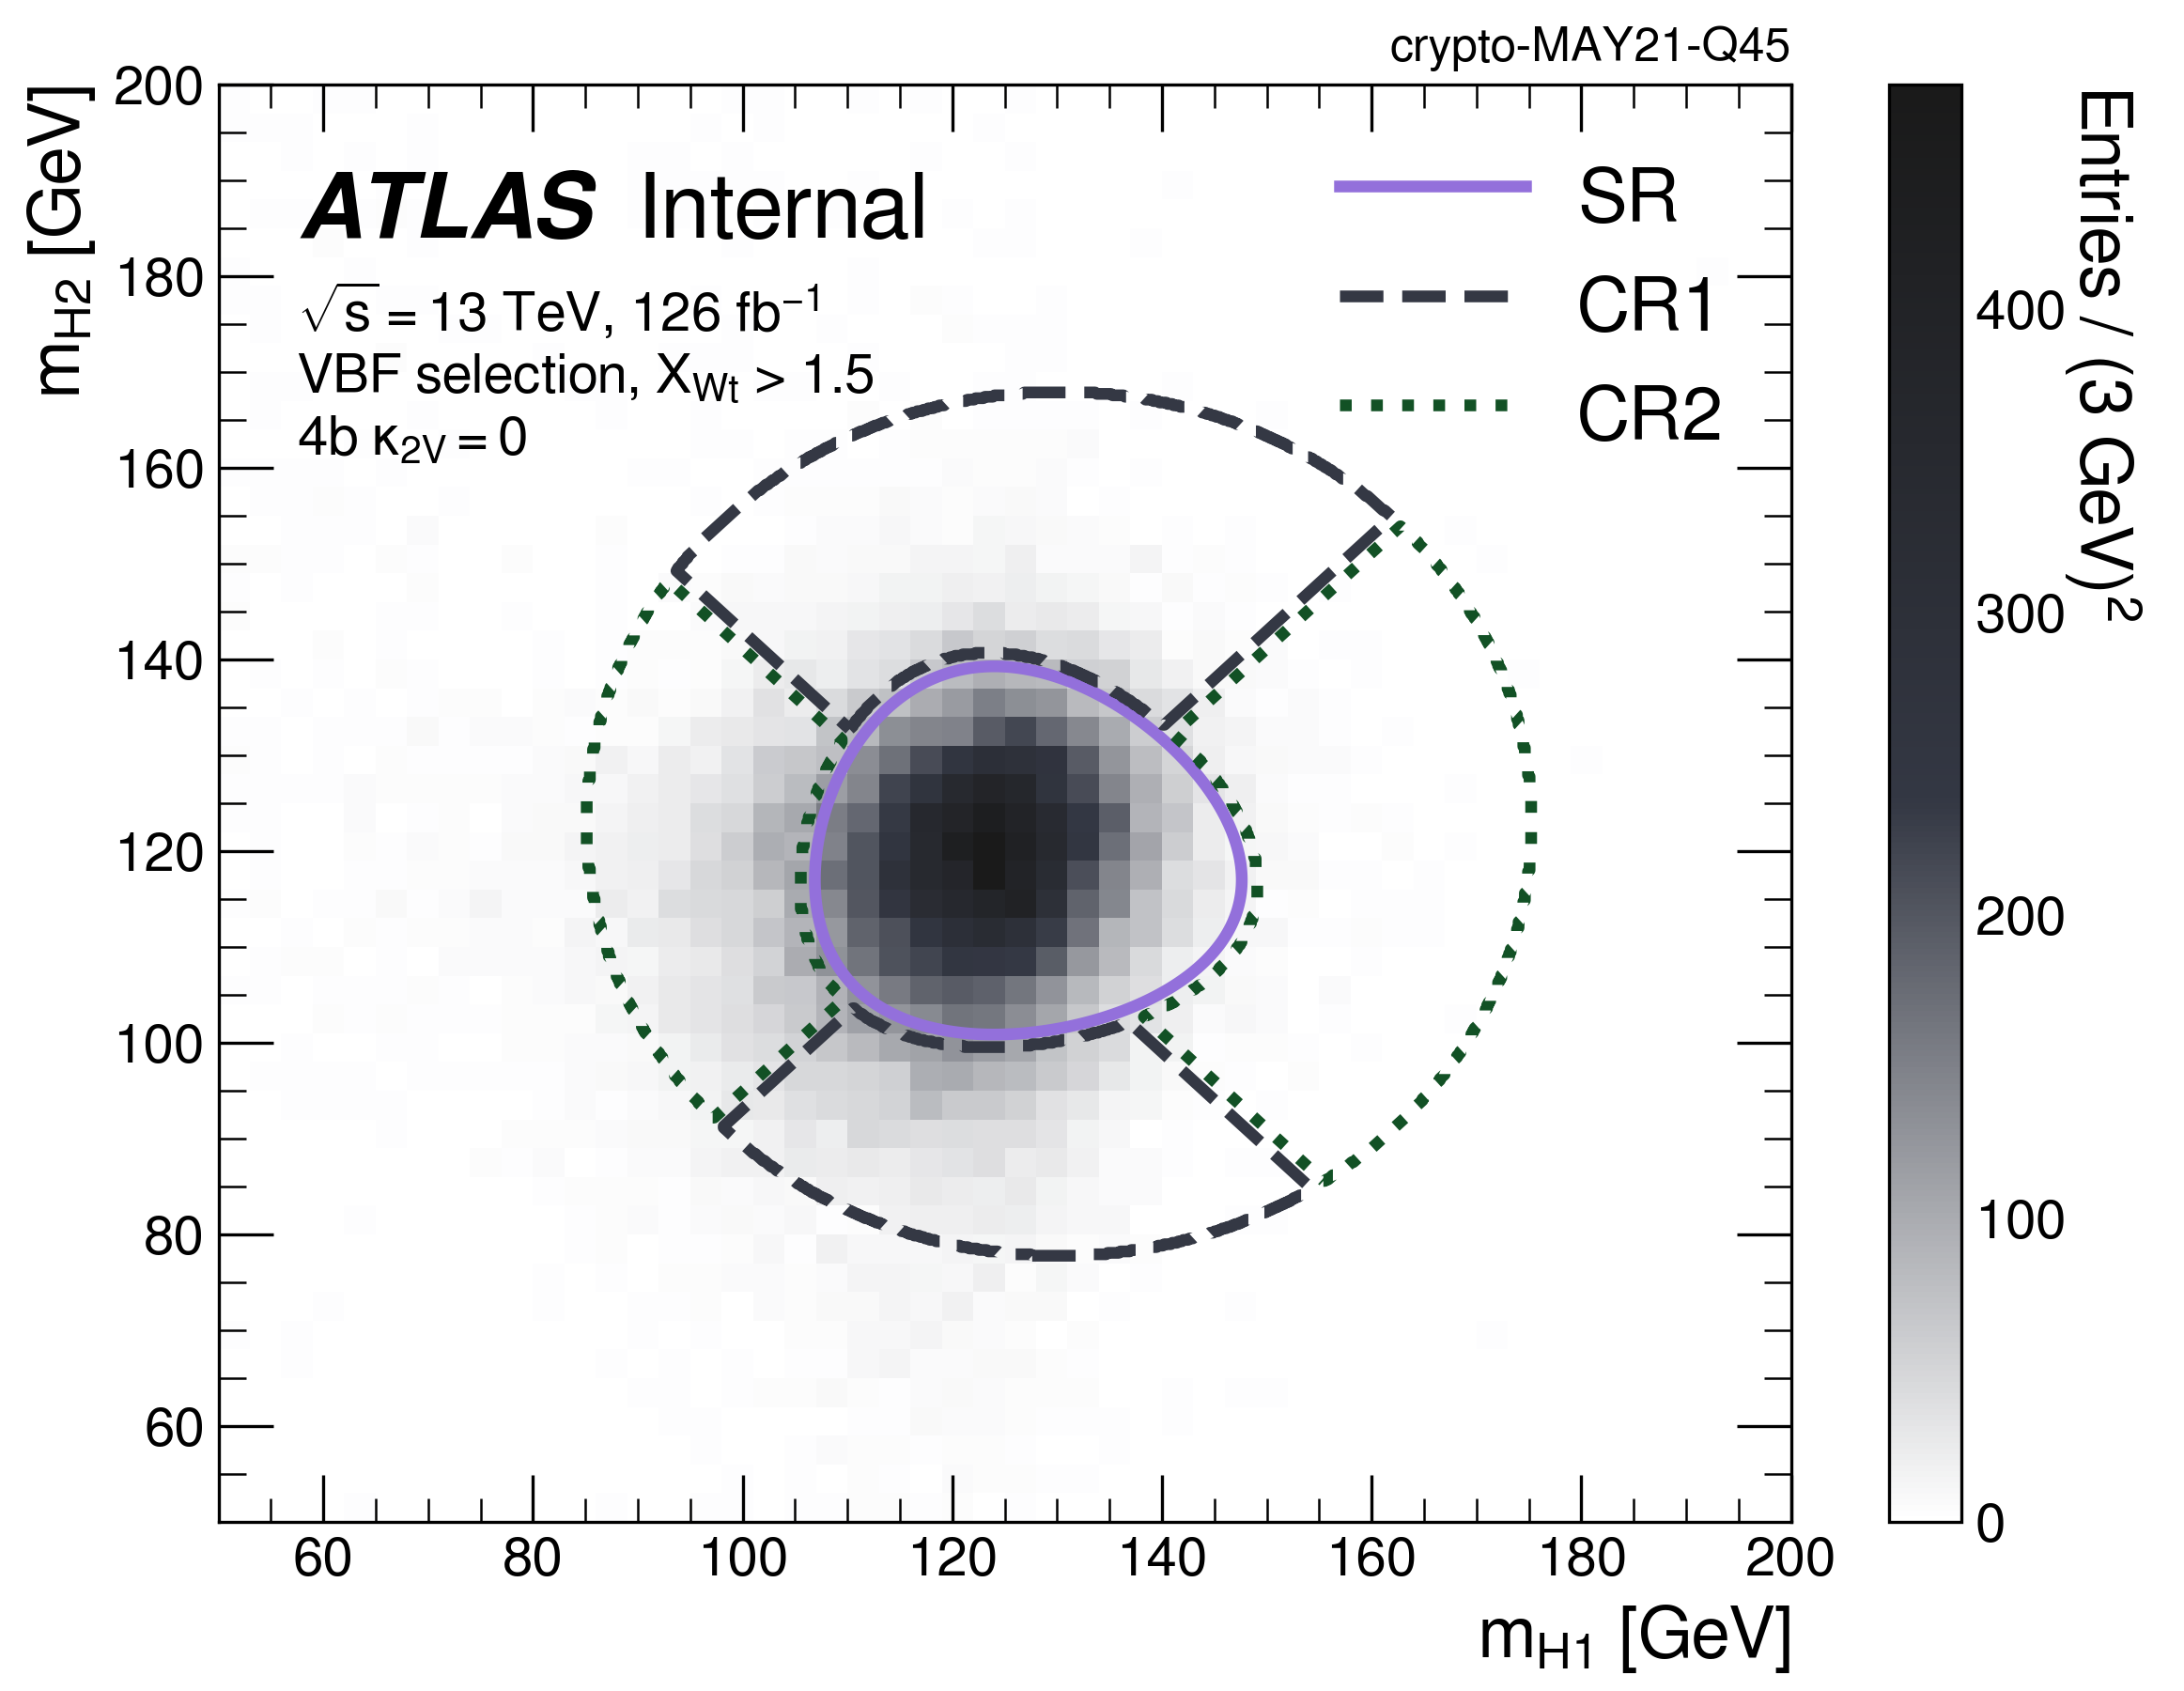
\includegraphics[width=0.4\textwidth]{figures/nr-int-note/selection/V3/massplane_sig_all_4b_vbf_Xwt_1.5_k2V_0.png}
 		\label{fig:VBF-massplanes-allYrs-k2V-0}
	}
	\caption{Selected Higgs Candidate signal mass planes.}
	\label{fig:massplanes-allYrs-signal}
\end{figure}

\begin{figure}[ht]
	\centering
	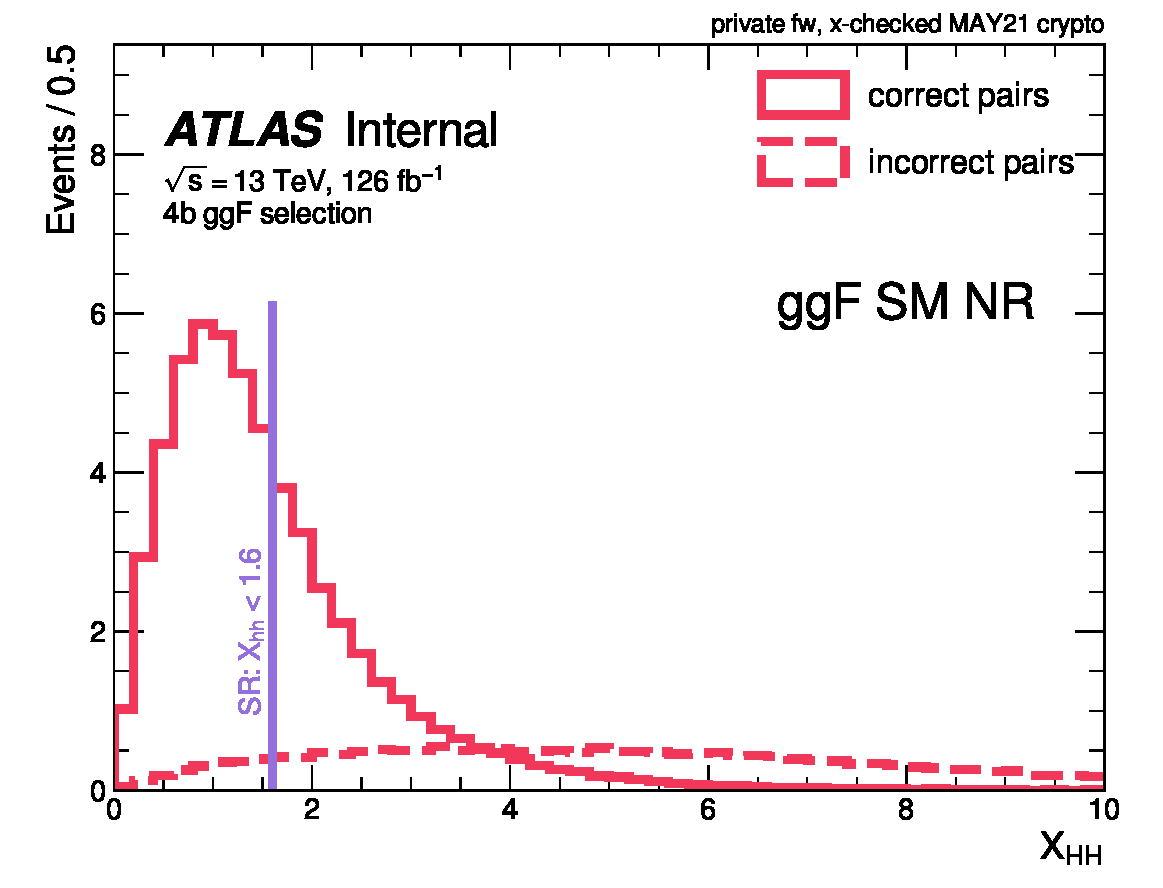
\includegraphics[width=0.4\textwidth]{figures/nr-int-note/selection/V3/X_hh-ggf-sm-4b.pdf}
	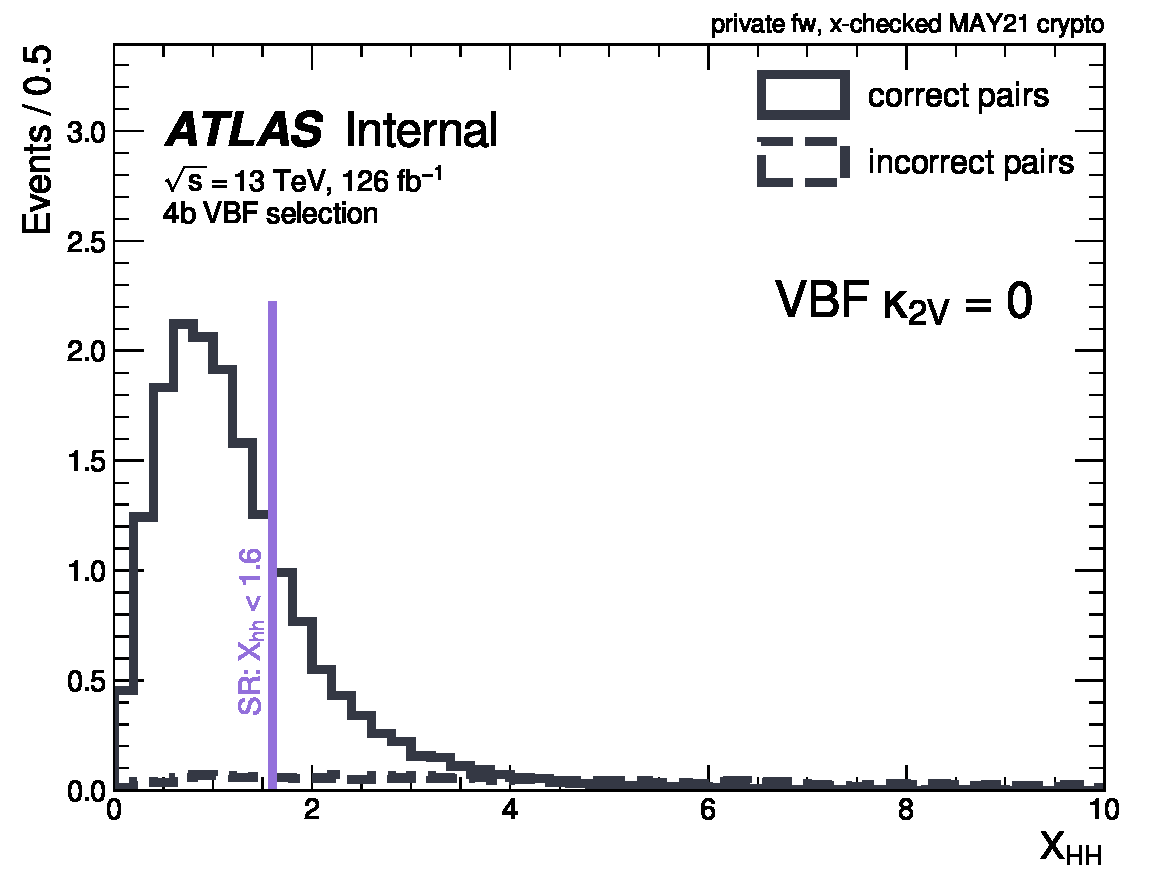
\includegraphics[width=0.4\textwidth]{figures/nr-int-note/selection/V3/X_hh-vbf-k2V_0-4b.pdf}
	\caption{Visualization of the \Xhh distribution for correctly and incorrectly paired events with the ggF (left) and VBF (right) analysis selections. The purple line indicates the SR defining cut.}
	\label{fig:ggF-Xhh}
\end{figure}

\begin{align}
	\text{SR} \quad &: \quad \Xhh < 1.6 \label{eq:sr} \\ 
	% \text{\textcolor{hh:darkblue}{CR1}/ \textcolor{hh:darkgreen}{CR2}}\ \text{Outer Edge} \quad &: \quad \sqrt{ \left(m_{\PH1} - 1.05 \cdot \SI{124}{\GeV}\right)^2 +  \left(m_{\PH2} - 1.05 \cdot \SI{117}{\GeV}\right)^2 } < \SI{45}{\GeV}  \label{eq:cr}
	\text{CR\ Inner\ Edge} \quad &: \quad \Xhh = 1.6 \label{eq:cr_in} \\
	\text{CR\ Outer\ Edge} \quad &: \quad \sqrt{ \left(m_{\PH1} - 1.05 \cdot \SI{124}{\GeV}\right)^2 +  \left(m_{\PH2} - 1.05 \cdot \SI{117}{\GeV}\right)^2 } = \SI{45}{\GeV}  \label{eq:cr_out}
\end{align}

\Fig{\ref{fig:massplanes-allYrs-data}} shows the blinded 4b data mass planes for the ggF and VBF selections, and the 2b data mass planes for the ggF and VBF selections. Note, the backgrounds for the 4b distributions are built from reweighted 2b data.

The key task for setting limits is correctly predicting the distributions for key discriminating variables in the SR. 
For this fully-hadronic final state analysis, we have a fully data driven background estimation method derived using events in a kinematically similar control region.
We define two control regions: Control Region 1 (CR1) and Control Region 2 (CR2). 
CR1 is used to derive the data-driven background estimate and CR2 is used to derive a systematic uncertainty associated with our methodology. 
These points will be expanded on in \Sect{\ref{sec:bkgdestimation}}. 
The region between the closed curves defined by \Eqn{\ref{eq:cr_in}} and \Eqn{\ref{eq:cr_out}} forms a band, within which CR1 and CR2 are defined. This region is orthogonal to the SR by design. This band is split into quadrants i.e. four sectors of roughly equal area. CR1 and CR2 are each defined as a pair of quadrants, where quadrants are paired such that they are on opposite sides of the band. The boundaries of CR1 and CR2 are shown in \Fig{\ref{fig:massplanes-allYrs-data}}.
This is a different choice comparing to the 4b resonant analysis~\cite{bbbbresolvedNote}, where rings of CR (and Validation Region) is used.
The new choice reduces potential signal contamination in resonant VR and has a better extrapolation since CR is closer to SR.
See \App{\ref{train-with-sig-inject}} for some studies.

\begin{figure}[ht]
	\centering
	\subfloat[Blinded 4b data for ggF selection]{
	     	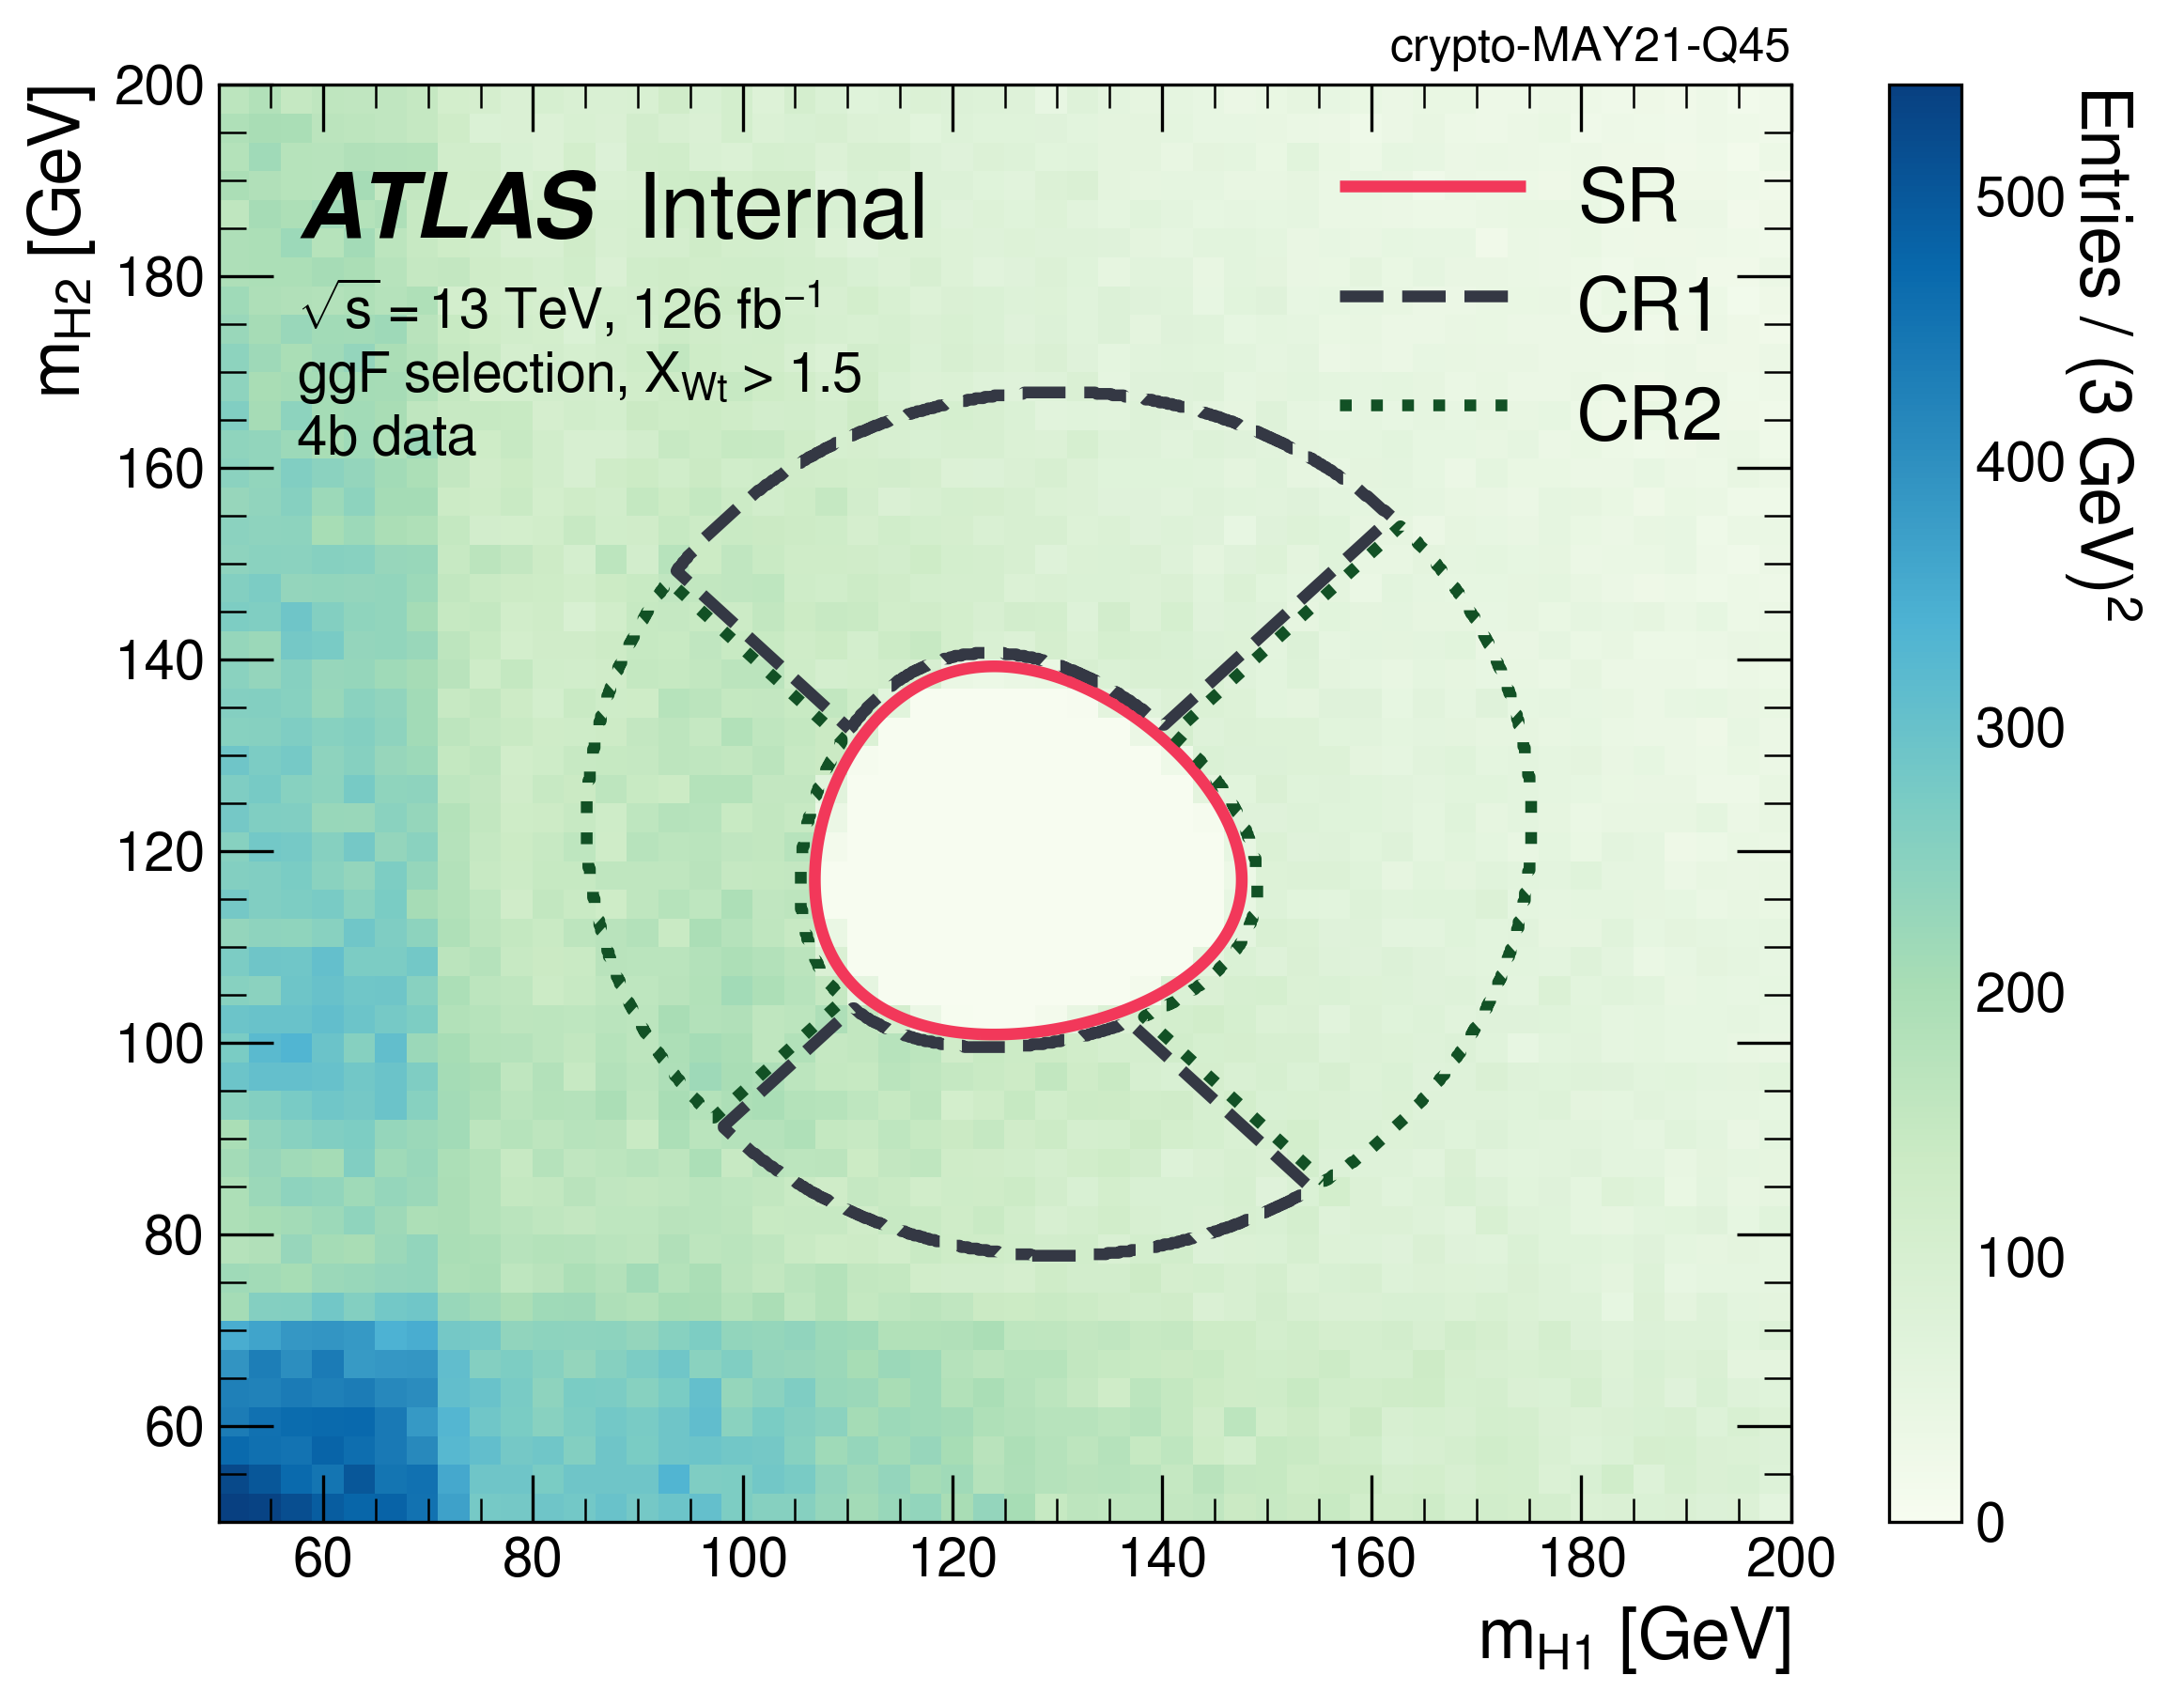
\includegraphics[width=0.4\textwidth]{figures/nr-int-note/selection/V2/massplane_dat_all_4b_ggf_Xwt_1.5.png}
		\label{fig:ggF-massplanes-allYrs-dat-4b}
	}
	\subfloat[Blinded 4b data for VBF selection]{
	     	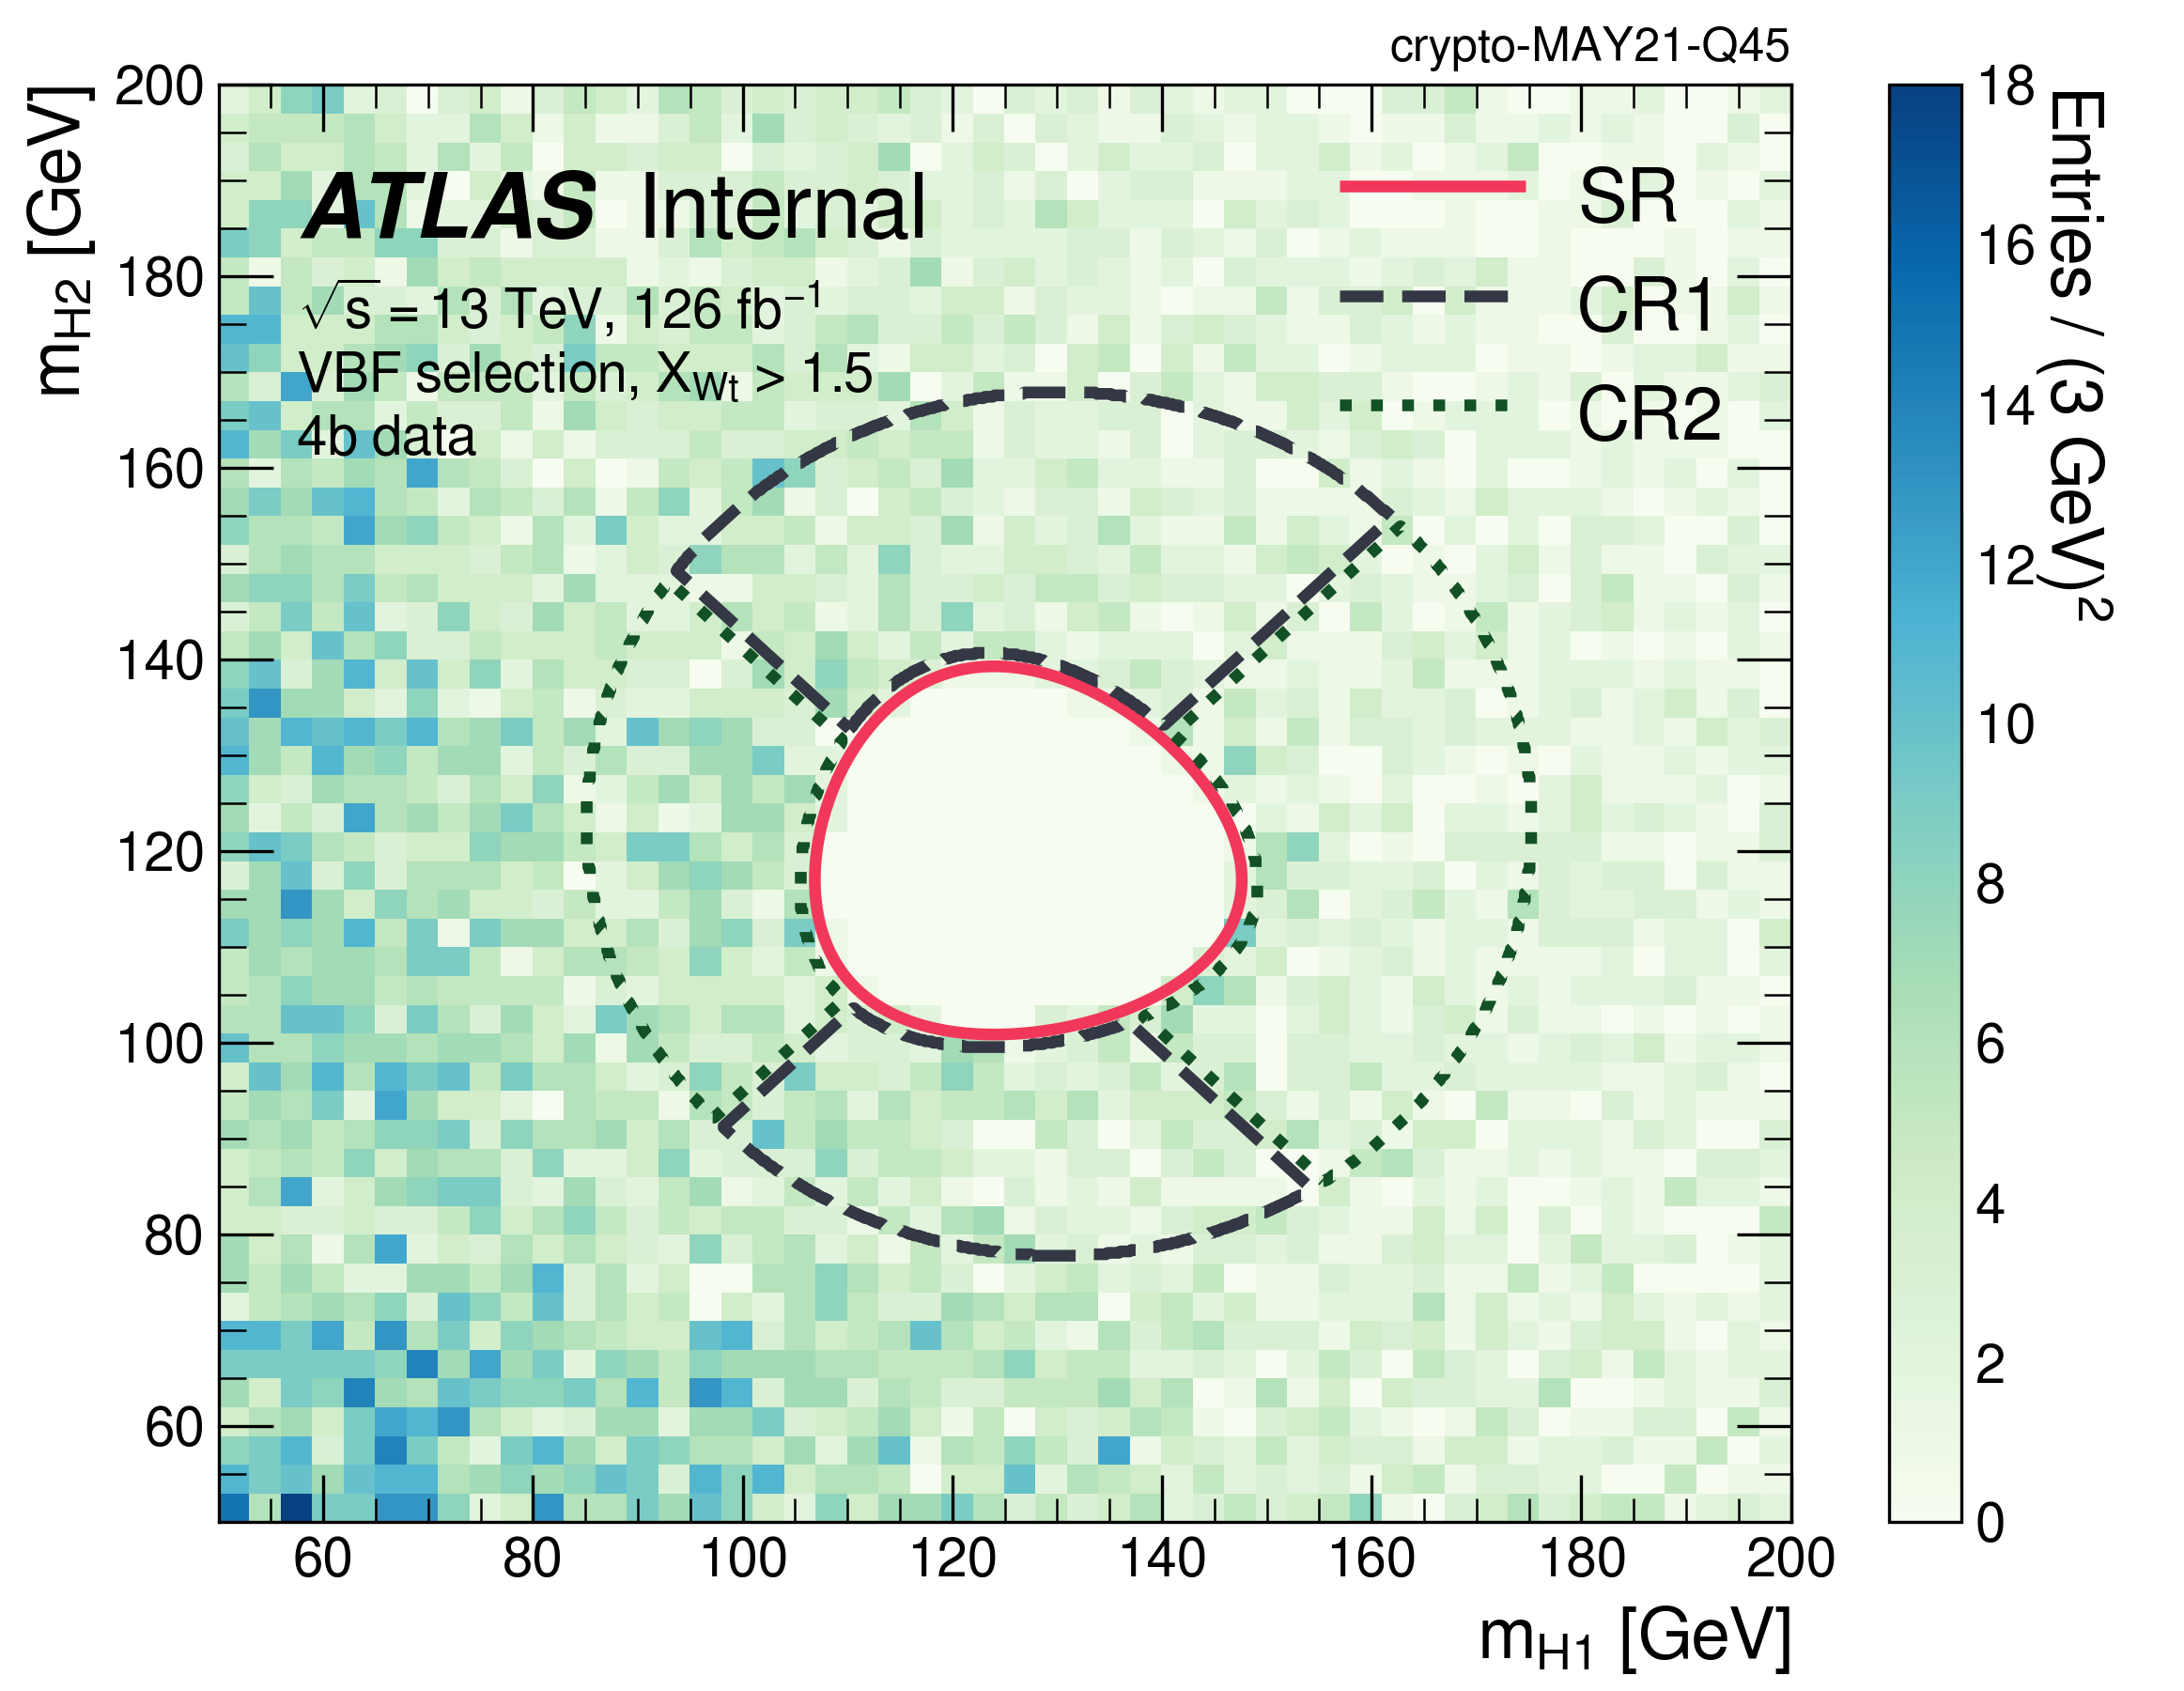
\includegraphics[width=0.4\textwidth]{figures/nr-int-note/selection/V2/massplane_dat_all_4b_vbf_Xwt_1.5.png} 
		\label{fig:VBF-massplanes-allYrs-dat-4b}
	}\\
	\centering
	\subfloat[2b data for ggF selection]{
	     	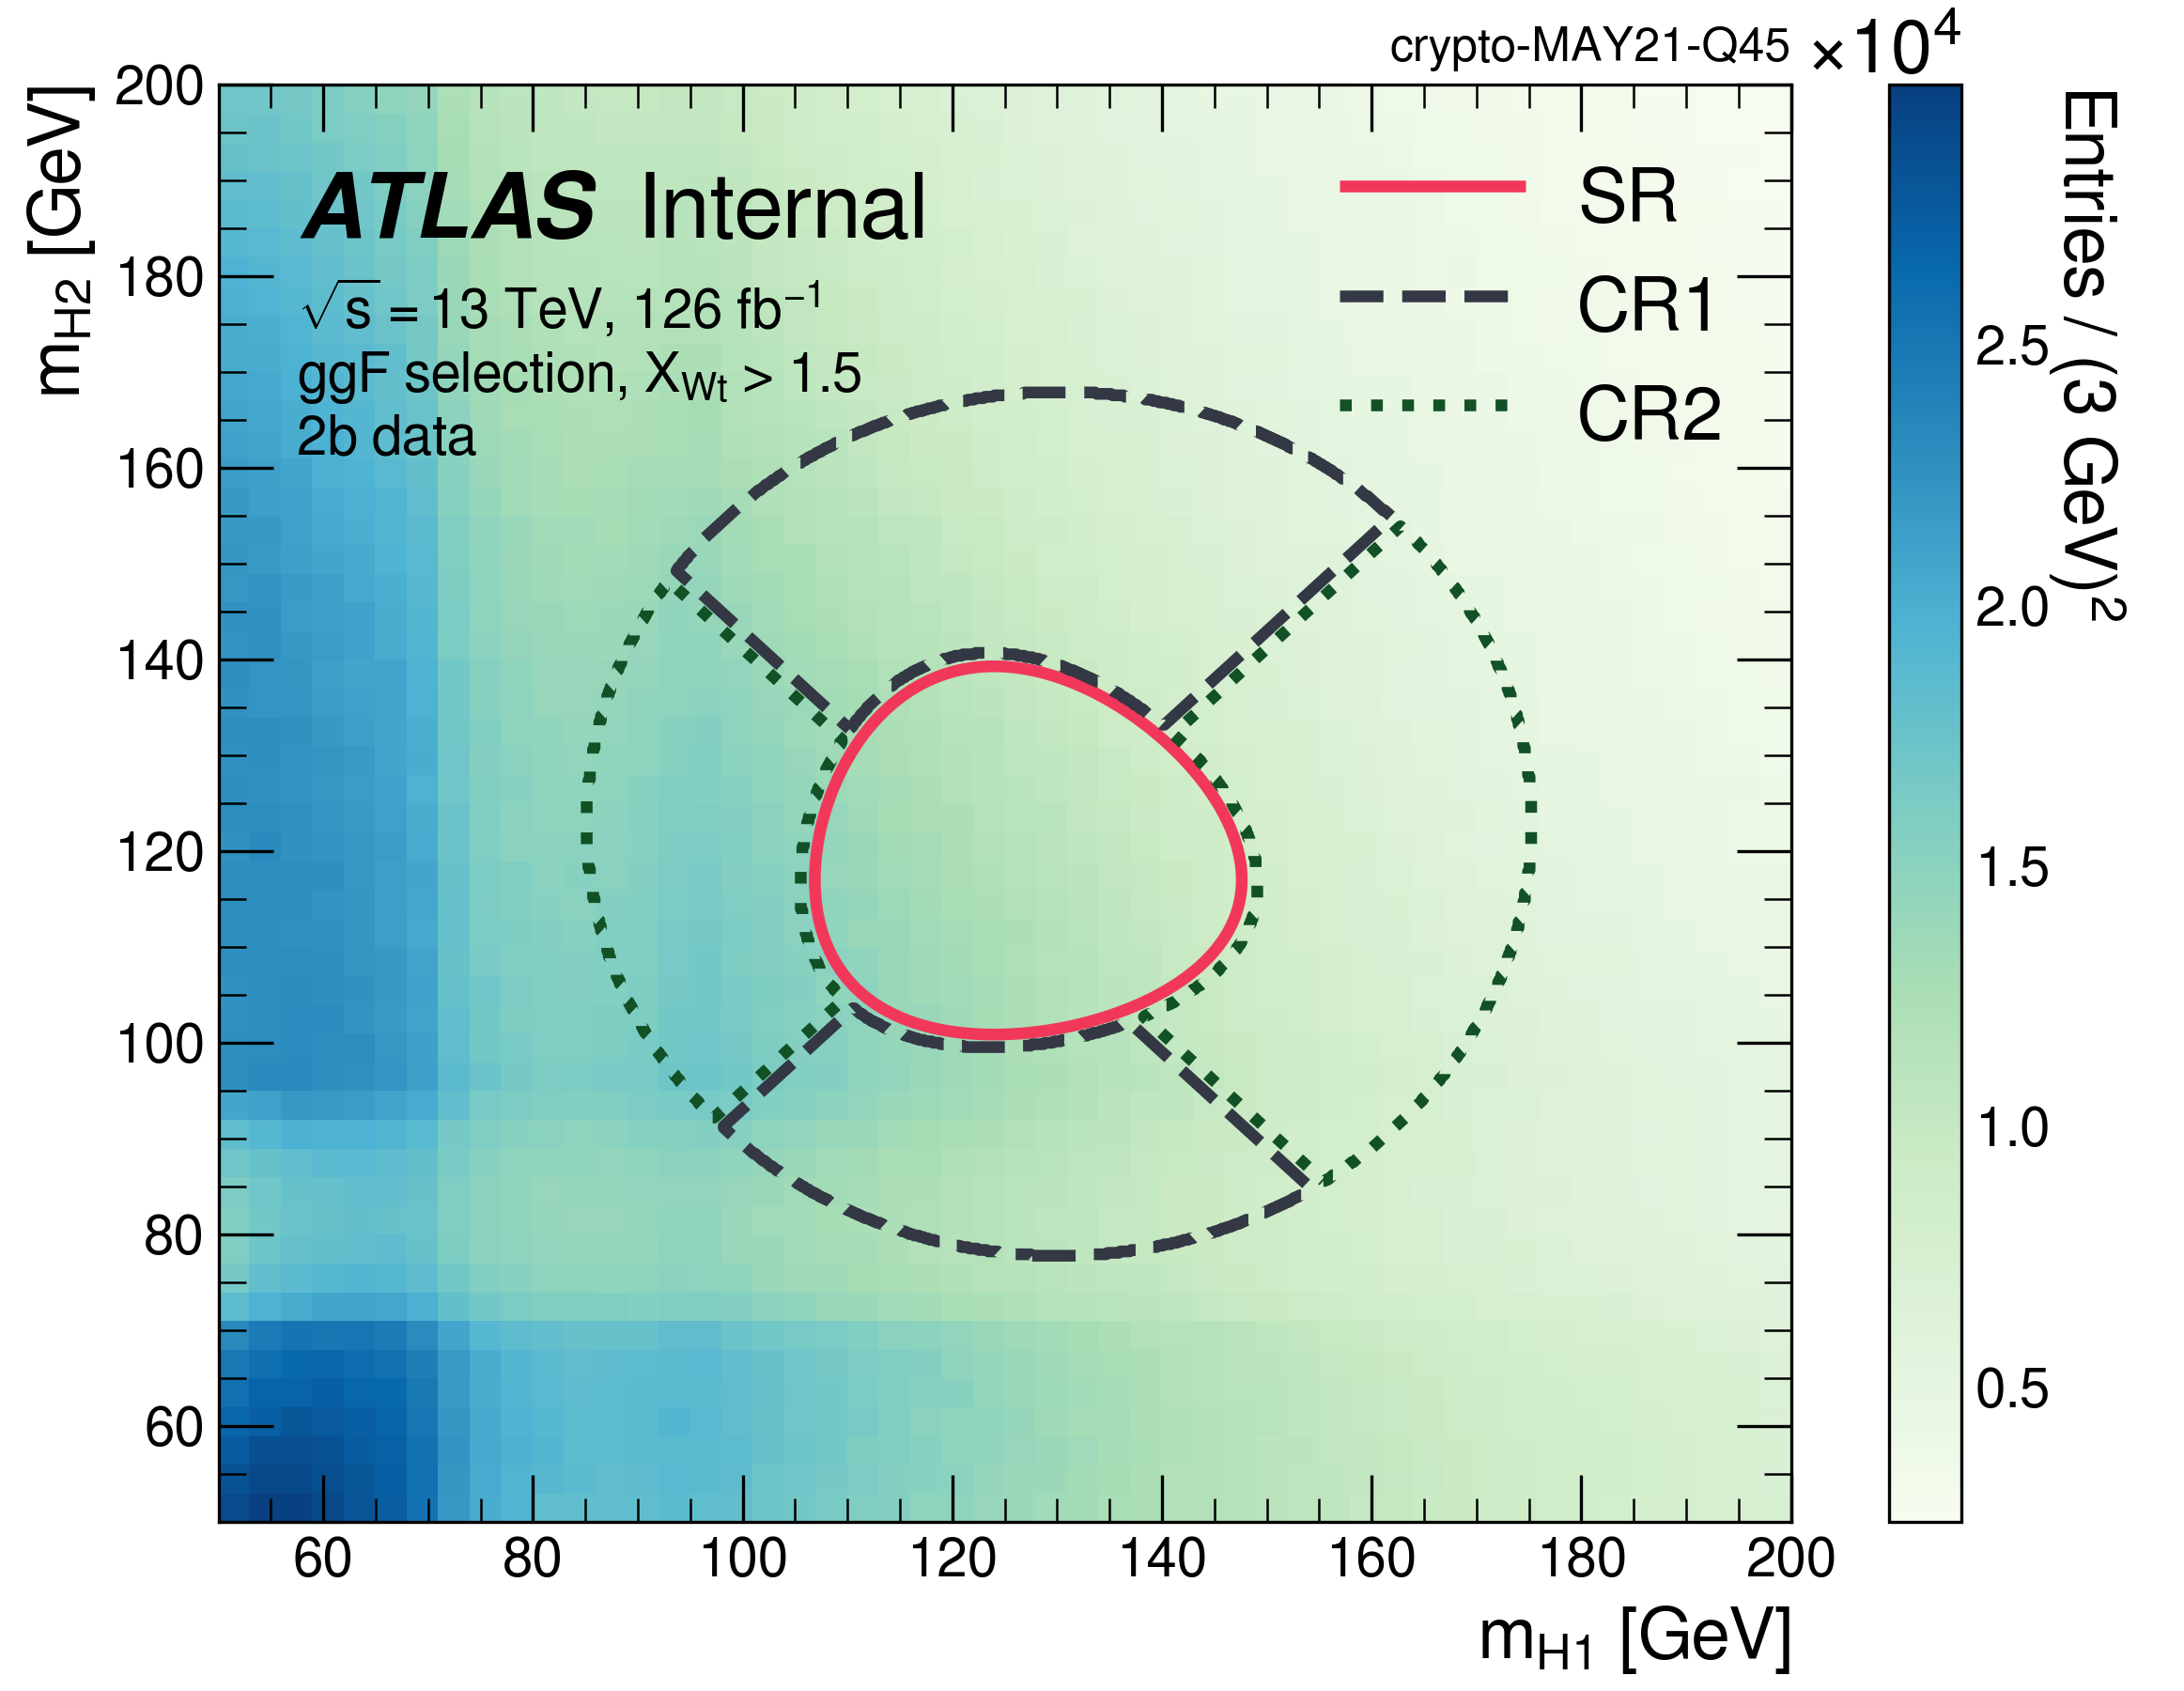
\includegraphics[width=0.4\textwidth]{figures/nr-int-note/selection/V2/massplane_dat_all_2b_ggf_Xwt_1.5.png}
		\label{fig:ggF-massplanes-allYrs-dat-2b}
	}
	\subfloat[2b data for VBF selection]{
	     	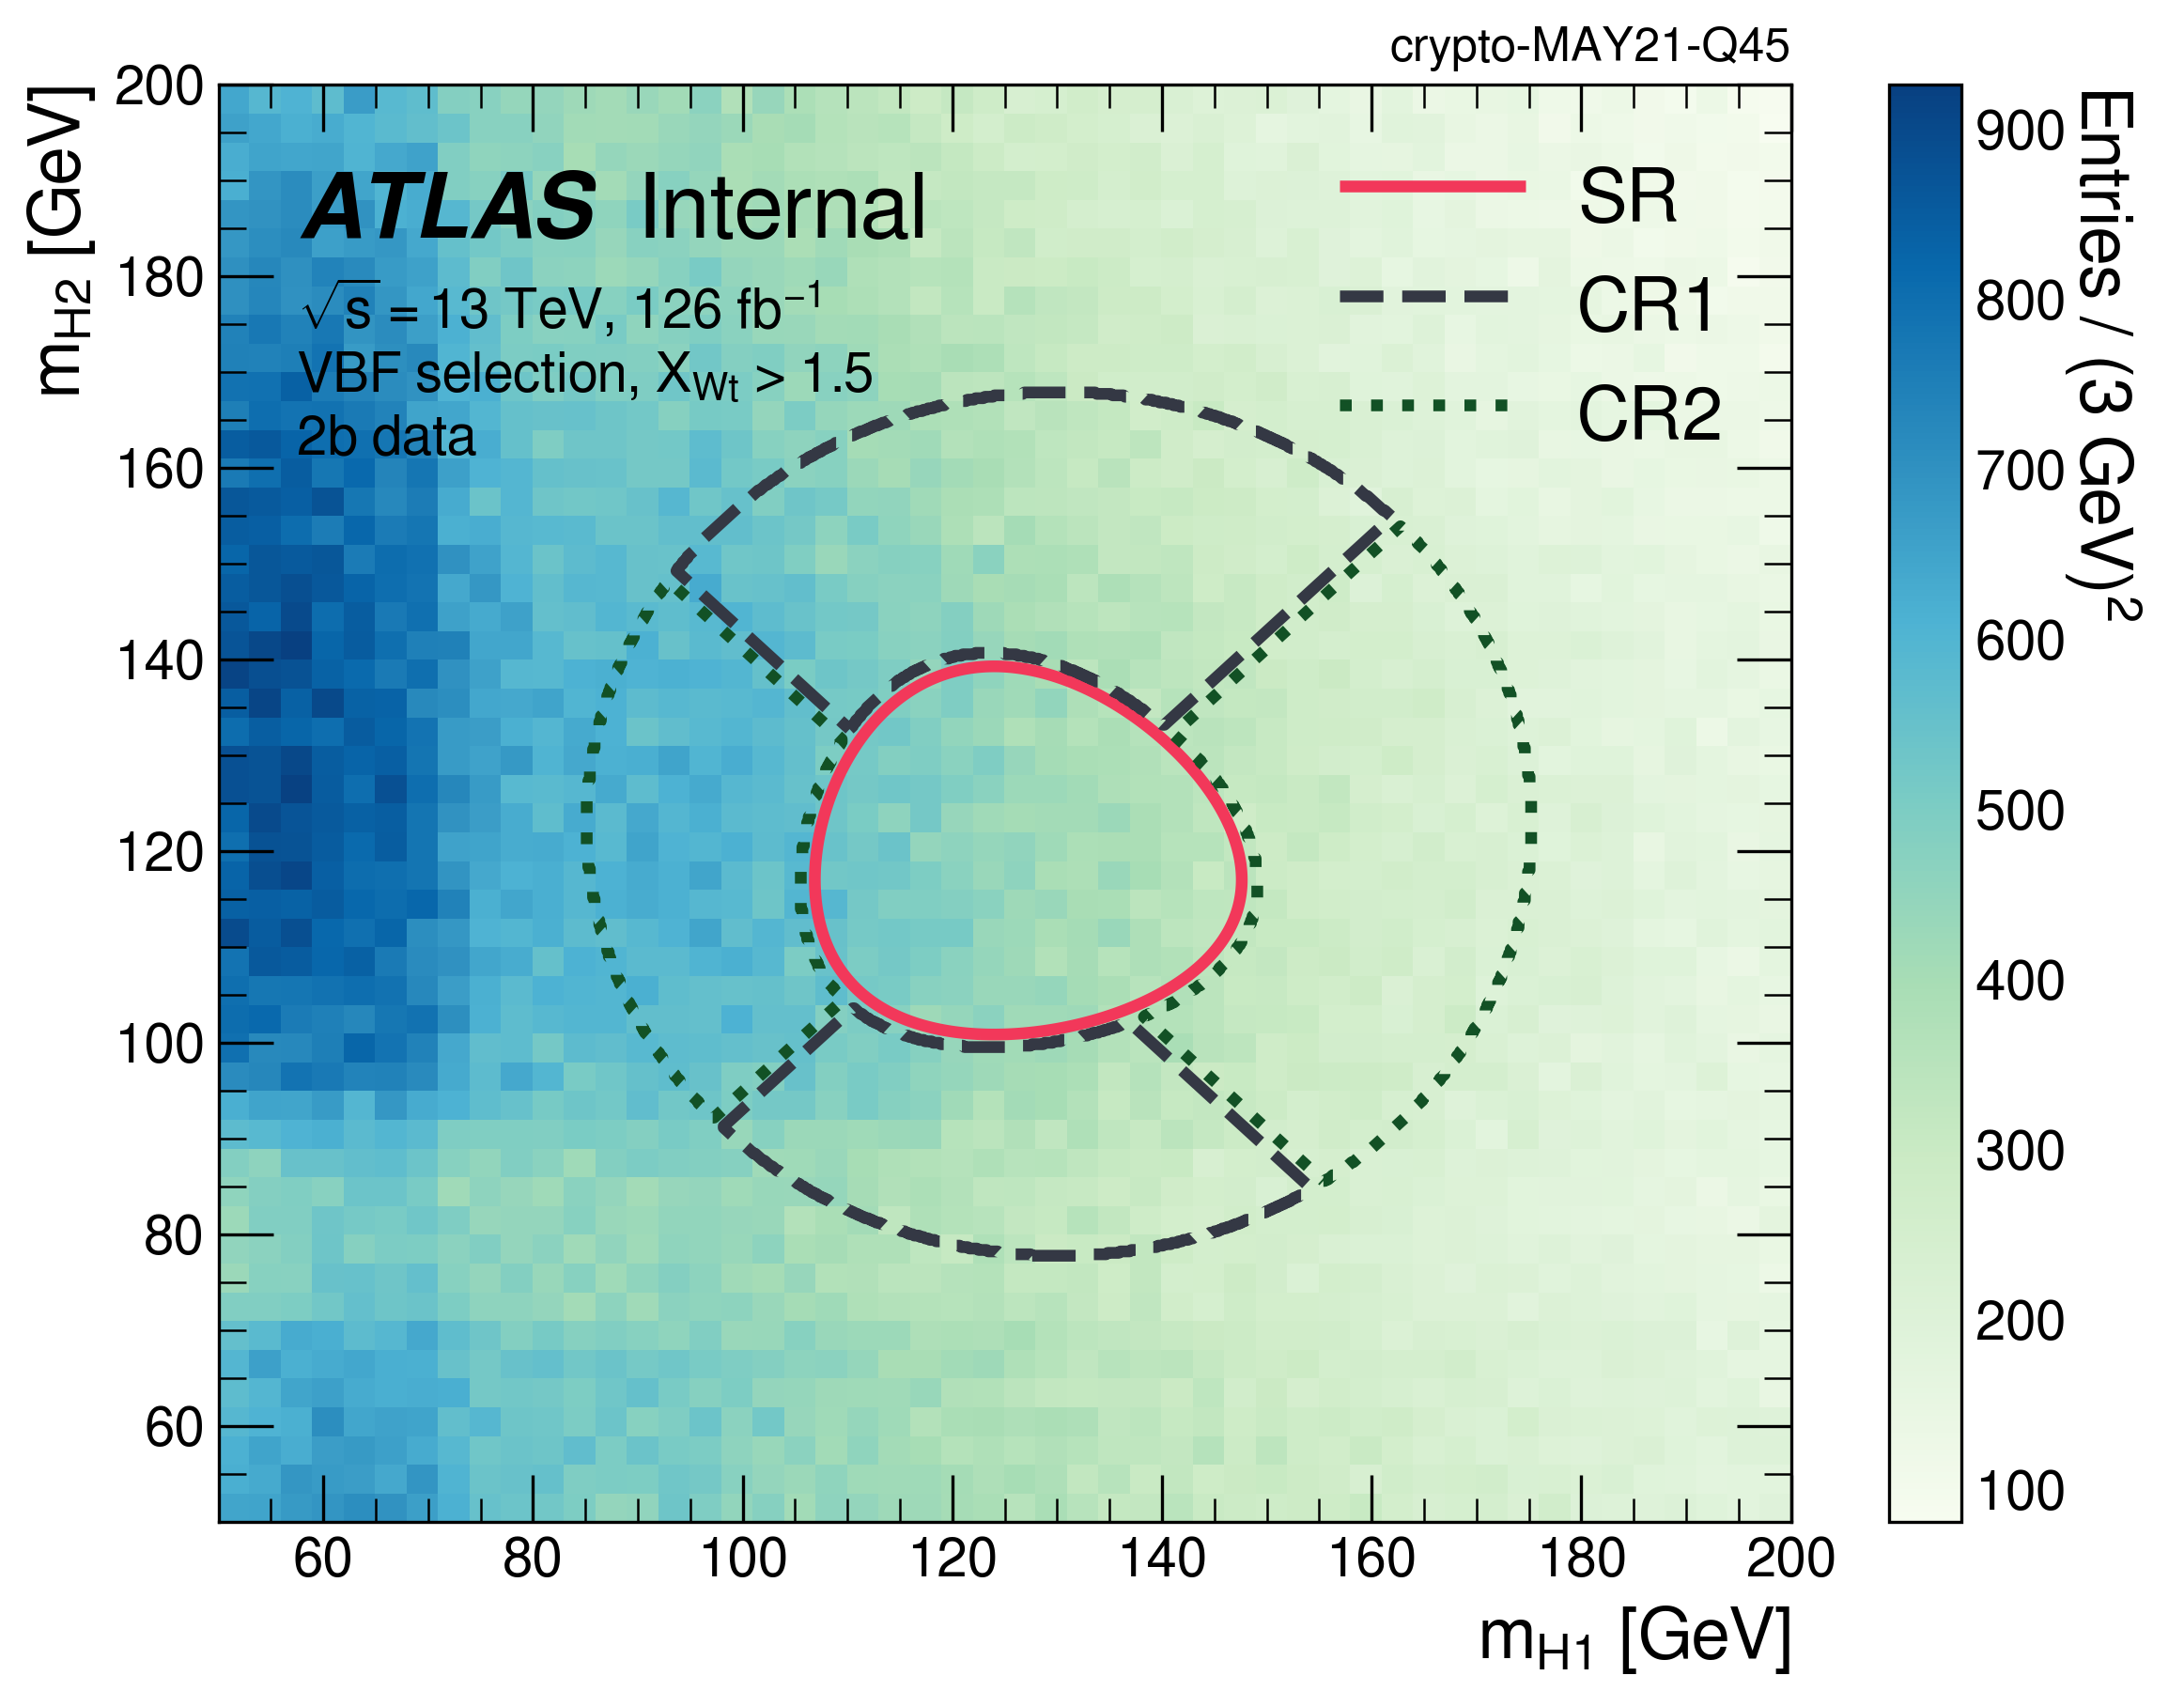
\includegraphics[width=0.4\textwidth]{figures/nr-int-note/selection/V2/massplane_dat_all_2b_vbf_Xwt_1.5.png} 
		\label{fig:VBF-massplanes-allYrs-dat-2b}
	}
	\caption{The Higgs Candidate massplanes for the ggF and VBF analysis selections.}
	\label{fig:massplanes-allYrs-data}
\end{figure}

The four quadrants that define CR1 and CR2 can be orientated in an infinite number of ways. The \Xwt cut applied in the selection acts like a \PW-mass veto for the constructed Higgs Candidates (HCs) causing a distinct drop in the number of events with $m_{h1}$ or $m_{h2}$ equal to $\sim$80 \GeV. In \Fig{\ref{fig:massplanes-allYrs-data}}, this effect can be observed as the two straight light-colored bands centered around $\sim$80 \GeV on the x and y-axes which stretch horizontally and vertically across the plot.\footnote{These mass planes before applying the \Xwt > 1.5 cut are shown in \Fig{\ref{fig:ggF-massplanes-Xwt}} and \Fig{\ref{fig:VBF-massplanes-Xwt}} for the respective ggF and VBF selections} The orientation of the quadrants shown in \Fig{\ref{fig:massplanes-allYrs-data}} was chosen such that these dips in the number of events equally impacted both CR1 and CR2.

Several different orientations were tested. In the studies conducted, different orientations were expressed as the angle between the x-axis and the closest CR1-CR2 boundary above the x-axis. Angles of \SI{0}{\degree}, \SI{30}{\degree}, \SI{45}{\degree} were compared and \SI{45}{\degree} was found to give better agreement 
in the 3b + 1 fail validation sample. Further investigation showed that this improvement stems from the \Xwt variable similarity, which is discussed in \App{\ref{app:sec:emd}}.

%CRs are defined by events passing the selection in \Eqn{\ref{eq:cr}}, where the steeply falling mass planes in \Fig{\ref{fig:massplanes-allYrs-data}} motivate the additional shift of 1.05 for the circle center for the means of the $(m_{H1}, m_{H2})$ 2b distributions to approximately match the 2b SR means. \todo{Need to check if this statement is still true with the new regions, or remove this motivation for the 1.05 shift.}


\clearpage

\section{Analysis Categories}
\label{sec:category}

\subsection{Definition of categories and binning}
\label{subsec:cat-motivation}

This analysis, as well as previous iterations, used the invariant mass of the HH system (\mhh) as the discriminating variable for the fit \cite{EXOT-2016-31,ATLAS-CONF-2021-035,HDBS-2018-18-witherratum}.\footnote{The previous ggF searches actually used corrected \mhh to scale the 4-vectors of the HCs to match the Higgs mass of 125 GeV. This modified definition of \mhh helped constrain the widths of the signal peaks in resonant searches.} A multi-variate algorithm (MVA) such as a BDT or NN would provide additional discrimination power; however, given our fully data driven background estimate, using a MVA may affect our ability to validate the modelling of the correlations between the input variables.
%As an example of this, the CMS non-resonant 4b analysis iterations have used a BDT for signal verses background discrimination, but see $2 \sigma$ tensions between the observed and expected limits due to the difficulty of accurately modeling the highest purity BDT bins \cite{CMS-HIG-17-017,CMS-PAS-HIG-20-005}. 
%Although a signal verses background BDT was investigated for the ggF analysis as well and improved the expected limits, 
As a compromise, a number of discriminating variables are used to define extra categories of $S / \sqrt{B}$ purity instead.

As alluded to in \Sect{\ref{sec:selection}}, \deta is a powerful discriminating variable for both the ggF and VBF analyses, and is used as a categorization variable for both these channels (see \Fig{\ref{fig:ggF-4b-deta-xhh-SR}} and \Fig{\ref{fig:vbf-detahh}}).
Specifics of the differences between the ggF and VBF categorization will be described in \Sect{\ref{subsubsec:ggF-cats}} and \Sect{\ref{subsubsec:VBF-cats}}, respectively, along with a visualization of \mhh distributions in each category.
A crucial step in implementing a categorization is ensuring the background within each category is well-modelled. In \Sect{\ref{sec:cats-CR1-validation}} are histograms of the background model in the CR1 training region. Good closure is observed.

Further tests of this categorization and validation of the background estimate are given in \Sect{\ref{sec:bkgvalidation}}.

Since the \mhh distribution is steeply falling, variable width histogram binning -- with narrower bins at low \mhh and wider bins at high \mhh\ -- is used in each of the categories. This allows the analysis to take advantage of the high \mhh events by having reasonable statistical uncertainties within these bins.

A logarithmic binning scheme was chosen. After defining the lowest bin edge, the second bin edge is set at (100 + X\%) $\times$ the lowest bin edge, where X is the specified percentage parameter. Then, the third bin edge is set at (100 + X\%) $\times$ the second bin edge. Bins of increasing width are added in this way until a upper threshold is surpassed. So, going from the lowest bin edge to the highest, the distance to a bin edge is a constant percentage increase on the previous bin edge. Note, the upper threshold is not the last bin edge. An algorithm is used to calculate the bin edges, and once it calculates a bin edge above this upper threshold, it adds it and stops.

Different logarithmic binning parameters are used for the ggF and VBF channels. These are shown in Table~\ref{tab:binning-hyperparameters}. These parameters were optimised to keep the relative error on the quadrature sum of the bootstrap and 2b Poisson components of the background model less than 30\%, whilst not making the bins so wide as to lose important shape information. This 30\% limit was chosen as it corresponds to the relative statistical error on 10 events, the rough threshold at which the asymptotic formulae used in limit setting are valid \cite{Cowan:2010js}. The plots demonstrating that the binning parameters satisfied this are shown in \App{\ref{app:binning}}.

For the ggF channel, the same binning was used across categories (see \Sect{\ref{subsubsec:ggF-cats}}), as the \mhh distributions differ little (as can be seen in \Fig{\ref{fig:ggF-4b-disc-log}} or \Fig{\ref{fig:ggF-4b-disc}}). For VBF, the length of the tails of the \mhh distribution in the two \deta categories differs greatly (\Fig{\ref{fig:vbf-mhh-same}}). As such, different parameters were used. The ggF histograms use bin boundaries rounded to the nearest 1~GeV and the VBF histograms use bin boundaries rounded to the nearest 5~GeV. For ggF, the underflow is included in the lowest bin and overflow is included in the highest bin. Whilst, for VBF, the underflow and overflows are defined as additional bins taking all events below and above the nominal binning.

\begin{table}[tbh]
\begin{center}
	\caption{Parameters used in the \mhh logarithmic binning algorithm. \textit{Min} refers to the starting lowest bin edge and \textit{Max} refers to the upper threshold after which the algorithm adds the last bin edge and stops.}
	\label{tab:binning-hyperparameters}
\begin{tabular}{| c | c | c | c | c |}
 \hline
 {} & Min [GeV] & Max [GeV] & Percentage [\%] & Rounded to Nearest [GeV] \\ 
 \hline\hline
 ggF All Categories & 280 & 950 & 9  & 1 \\ 
 \hline
 VBF low \deta & 280 & 890 & 10 & 5\\
 \hline
 VBF high \deta & 290 & 1470 & 9 & 5\\
 \hline
\end{tabular}
\end{center}
\end{table}

Another method for choosing the binning in \mhh was tested. This was based on an algorithm that systematically merged bins until the statistical uncertainty was under 30\%. This more flexible method resulted in more complicated binning scheme but very close significance and limits, giving us confidence that our simplified category choices are close to optimal.

\subsubsection{ggF categories}
\label{subsubsec:ggF-cats}

The ggF channels are categorized in two variables -- \deta and \Xhh. These variables are already cut on in the ggF channel -- \deta < 1.5 for the QCD background rejection and \Xhh < 1.6 for the SR definition.
The distributions of these two variables of background prediction in the SR are shown in \Fig{\ref{fig:ggF-4b-deta-xhh-SR}}, with overlaid the signal shapes. 
Since the background \deta distribution is flat, three equally spaced \deta bins were chosen between 0 and 1.5. Additionally, two \Xhh bins were defined, with the boundary of 0.95 chosen to equally split the correctly paired signal events. This boundary choice also optimized $S / \sqrt{B}$ significance for the SM NR ggF signal.

\begin{figure}[ht]
	\centering
	\subfloat[All year merged: 4b ggF \deta]{ 
	    	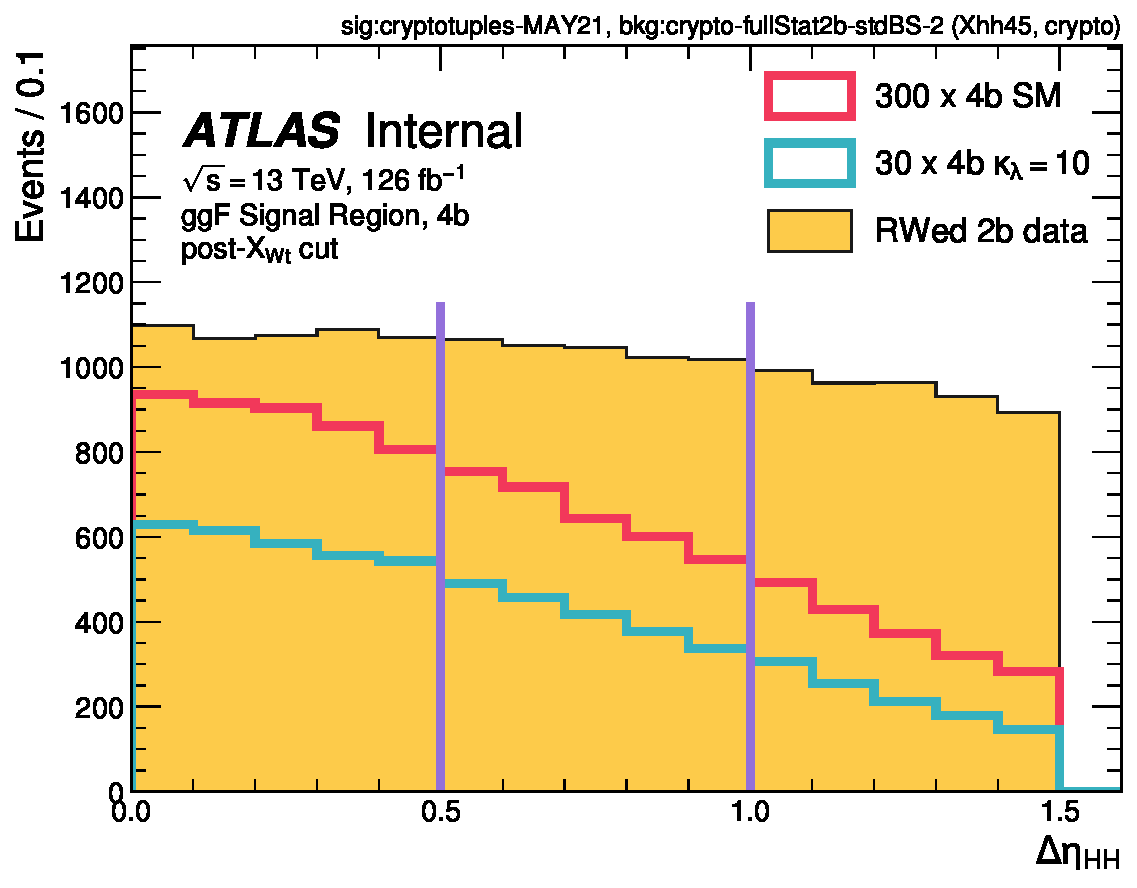
\includegraphics[width=0.4\textwidth]{figures/nr-int-note/category/V3/dEta_hh_sr_sig_bkg_4b_allyears}
	}
	\subfloat[All year merge: 4b ggF \Xhh]{ 
	    	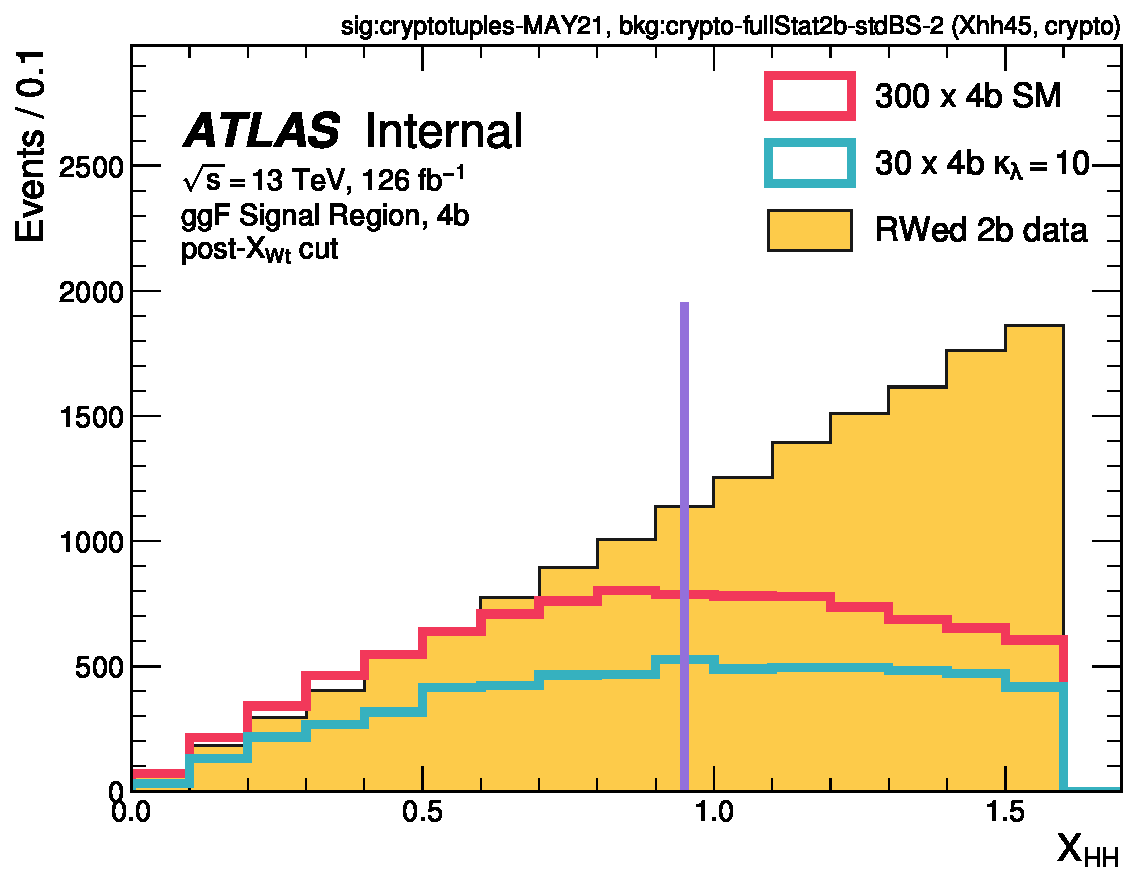
\includegraphics[width=0.4\textwidth]{figures/nr-int-note/category/V3/X_hh_sr_sig_bkg_4b_allyears}
	} 
	\caption{Distributions of the variables used for categorization in the ggF channel.
	Years are merged.
	To visualize the signals they are scaled by $\alpha = 100$ and 10 for the SM NR and $\kappa_\lambda$ = 10 signals, respectively.}
	\label{fig:ggF-4b-deta-xhh-SR}
\end{figure}

As discussed in \Sect{\ref{sec:bkgdestimation}}, the ggF background estimate is derived separately for the years, so we also fit the years separately as visualized in the 4b ggF histograms in \Fig{\ref{fig:ggF-4b-disc-log}}, with the SM and $\kappa_\lambda$ = 10 signals overlaid. The subpanels on these plots show the $S / \sqrt{B}$ significance to visualize which categories drive the sensitivity of the fit.
The signal peaks for the lower \deta, \Xhh values, so these are the higher purity categories that drive our significance.
The same plots with a linear y-axis are shown in \Fig{\ref{fig:ggF-4b-disc}}.

\begin{figure}[ht]
	\centering
	\subfloat[2016: 4b ggF]{ 
	    	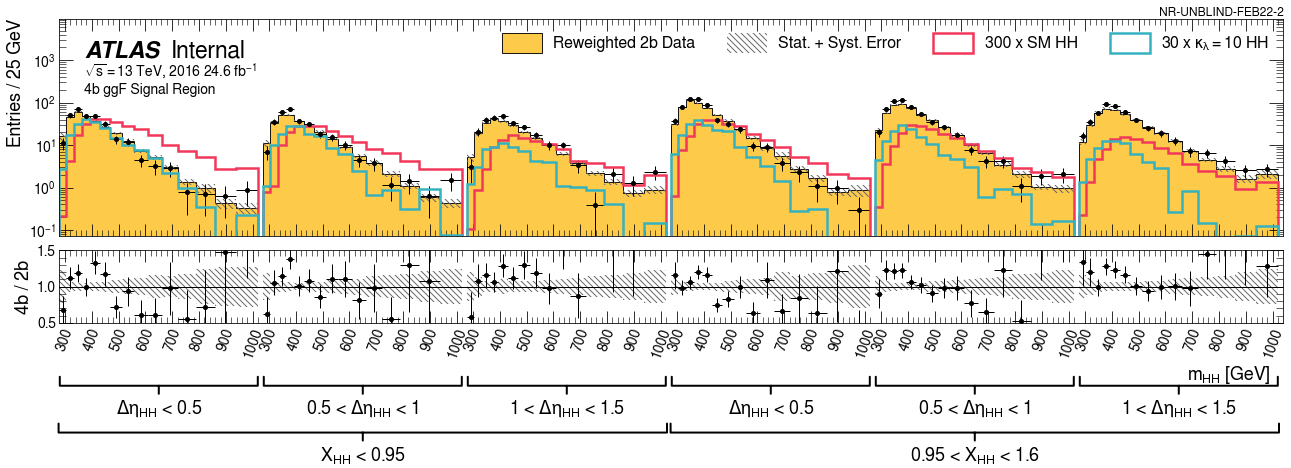
\includegraphics[width=\textwidth]{figures/nr-int-note/category/V4/m_hh_ggF_3_dEta_2_Xhh_ggF_16_4b_log.png}
		\label{fig:ggF-16-4b-log}
	} \\
	\subfloat[2017: 4b ggF]{ 
	    	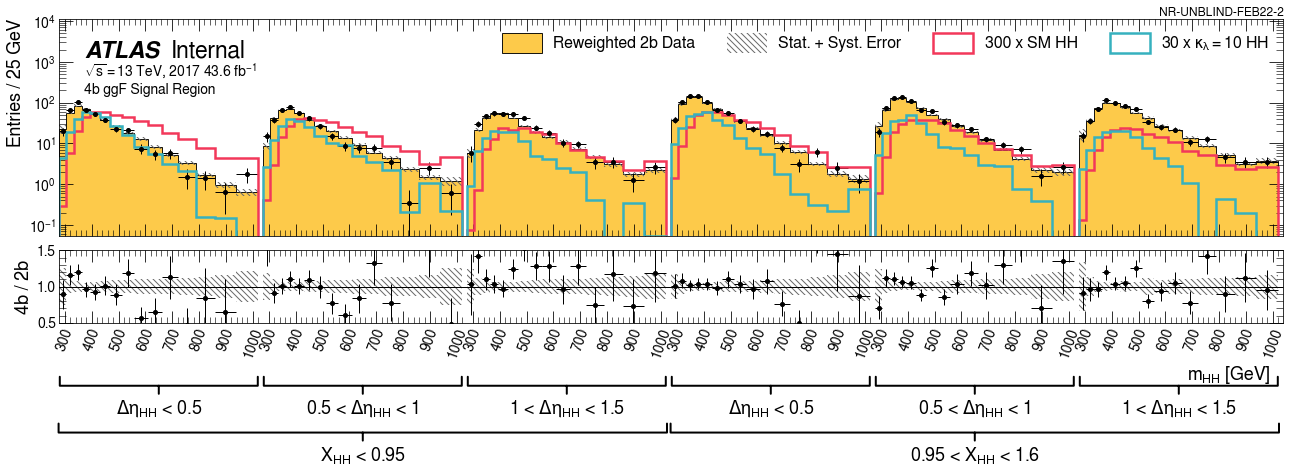
\includegraphics[width=\textwidth]{figures/nr-int-note/category/V4/m_hh_ggF_3_dEta_2_Xhh_ggF_17_4b_log.png}
		\label{fig:ggF-17-4b-log}
	} \\
	\subfloat[2018: 4b ggF]{ 
	    	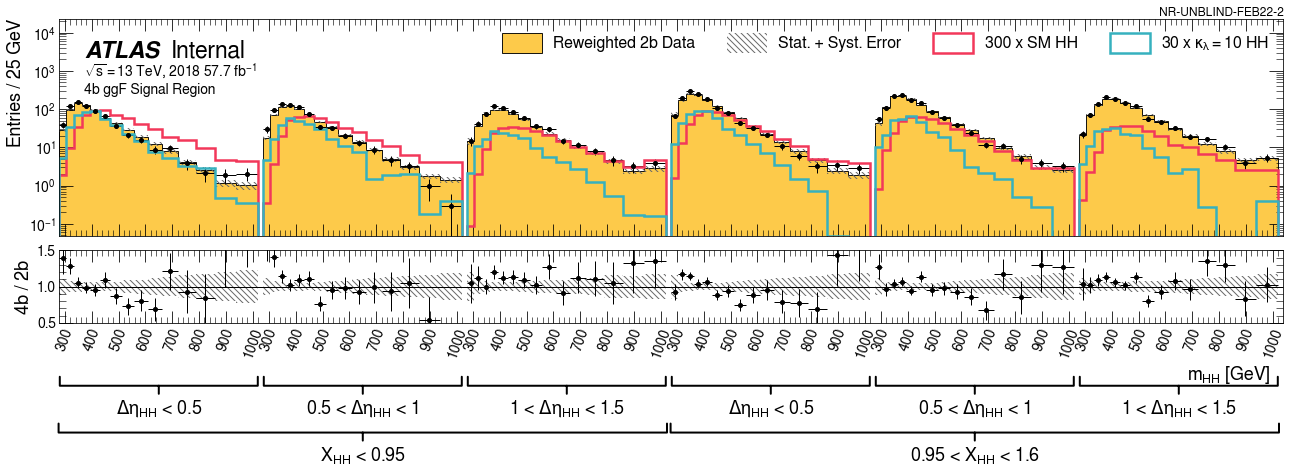
\includegraphics[width=\textwidth]{figures/nr-int-note/category/V4/m_hh_ggF_3_dEta_2_Xhh_ggF_18_4b_log.png}
 		\label{fig:ggF-18-4b-log}
	}
	\caption{4b \ ggF background and selected signal histograms for 2016, 2017, and 2018 with the proposed binning and categorization. To visualize the signals they are scaled by $\alpha = 100$ and 10 for the SM NR and $\kappa_\lambda$ = 10 signals, respectively.}
	\label{fig:ggF-4b-disc-log}
\end{figure}

\begin{figure}[ht]
	\centering
	\subfloat[2016: 4b ggF]{ 
	    	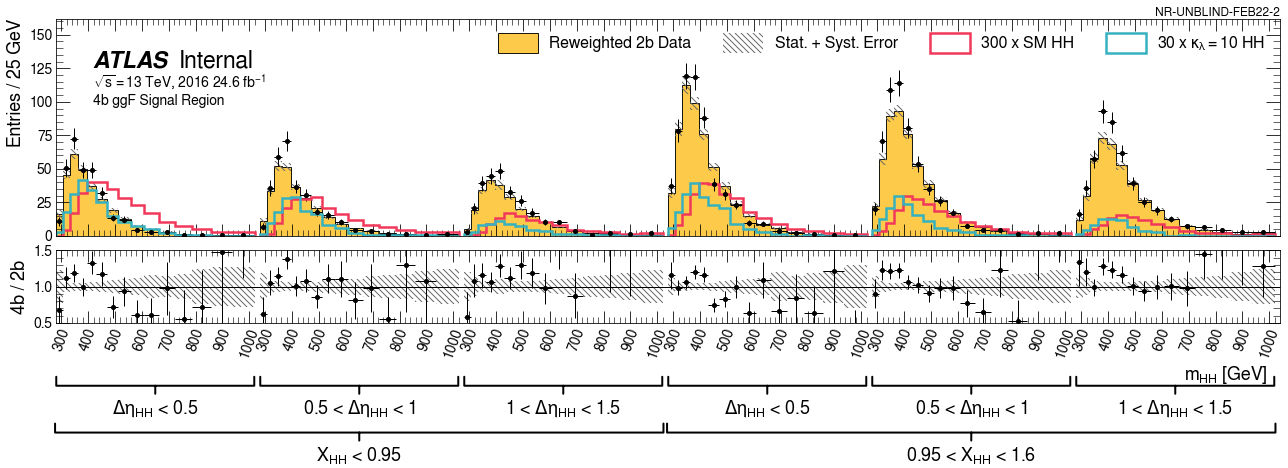
\includegraphics[width=\textwidth]{figures/nr-int-note/category/V4/m_hh_ggF_3_dEta_2_Xhh_ggF_16_4b.png}
		\label{fig:ggF-16-4b}
	} \\
	\subfloat[2017: 4b ggF]{ 
	    	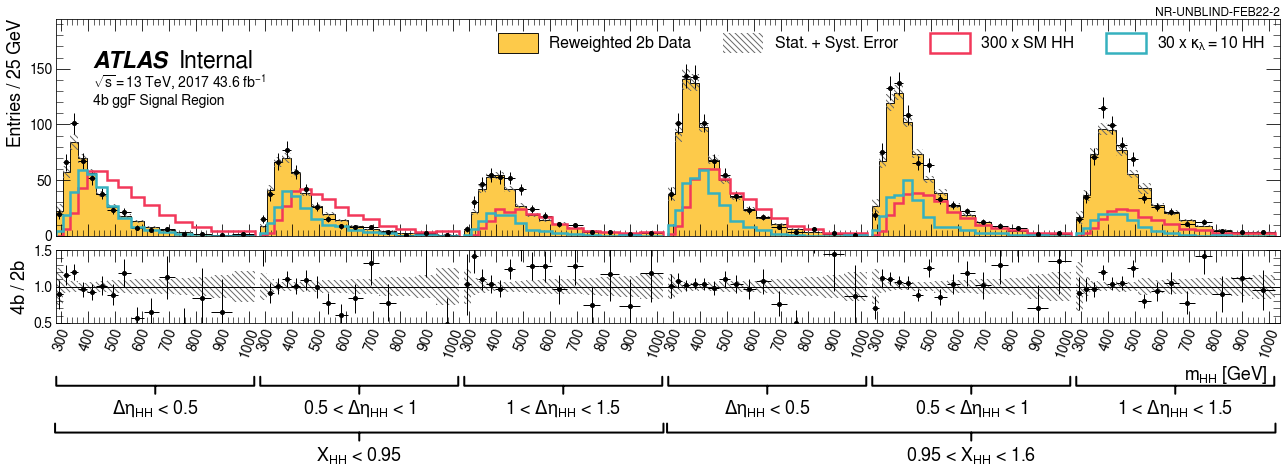
\includegraphics[width=\textwidth]{figures/nr-int-note/category/V4/m_hh_ggF_3_dEta_2_Xhh_ggF_17_4b.png}
		\label{fig:ggF-17-4b}
	} \\
	\subfloat[2018: 4b ggF]{ 
	    	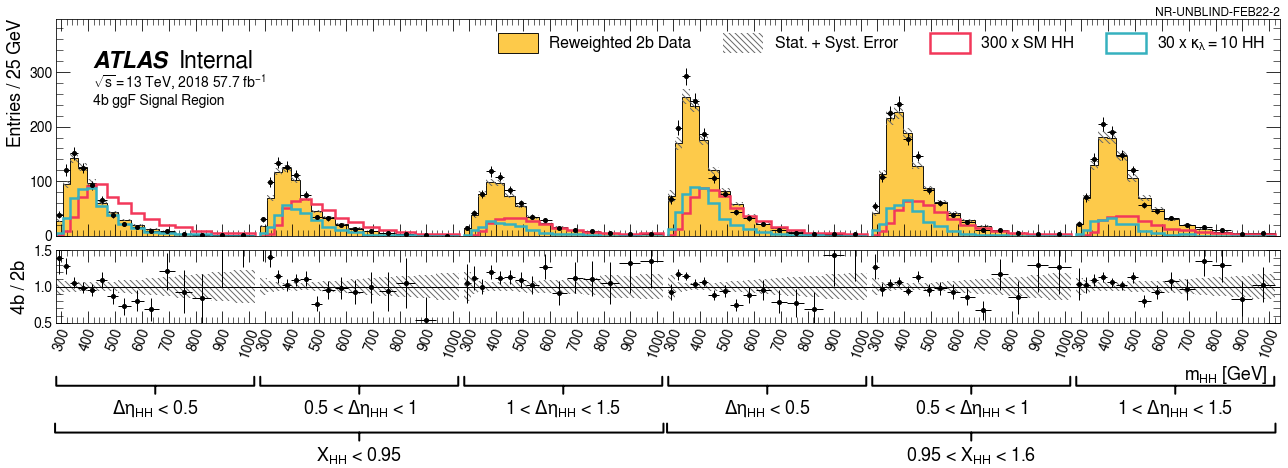
\includegraphics[width=\textwidth]{figures/nr-int-note/category/V4/m_hh_ggF_3_dEta_2_Xhh_ggF_18_4b.png}
 		\label{fig:ggF-18-4b}
	}
	\caption{4b \ ggF background and selected signal histograms for 2016, 2017, and 2018 with the proposed binning and categorization. To visualize the signals they are scaled by $\alpha = 100$ and 10 for the SM NR and $\kappa_\lambda$ = 10 signals, respectively.}
	\label{fig:ggF-4b-disc}
\end{figure}


%\Figure{\ref{fig:ggF-4b-disc-srs}} shows the histograms inclusive for the years, but separately visualizing the categories for the inside (\Xhh < 0.95) and outside (0.95 < \Xhh < 1.6) SRs.
% Visualizing the 4b discriminant separately as two SRs
% Commented out b/c non-trivial edits w/ our BS prescription
%\foreach \btag in {4b}{
%    \begin{figure}[ht]
%        	\centering
%        	\subfloat[2016--2018: \ \btag \ ggF SRin]{ 
%        	    	\includegraphics[width=\textwidth]{m_hh_ggF_3_dEta_2_Xhh_ggF_all_\btag_SRin.png}
%        	} \\
%        	\subfloat[2016--2018: \ \btag \ ggF SRout]{ 
%        	    	\includegraphics[width=\textwidth]{m_hh_ggF_3_dEta_2_Xhh_ggF_all_\btag_SRout.png}
%        	} \\
%        	\caption{\btag \ ggF background and selected signal histograms stacking the years (2016-2018) with the proposed binning and categorization. To visualize the signals they are scaled by $\alpha = 300$ and 10 for the SM NR and $\kappa_\lambda$ = 30 signals, respectively.}
%        	\label{fig:ggF-\btag-disc-srs}
%    \end{figure}
%}

\FloatBarrier
\clearpage

\subsubsection{VBF categories}
\label{subsubsec:VBF-cats}

%The VBF analysis has a single categorization based upon the pseudorapidity difference between the two reconstructed Higgs bosons, $\deta$.
The VBF analysis has a single categorization based on \deta.
The boundary for the categorization is 1.5, chosen as it satisfied the balance between maximizing significance and maintaining the accuracy of the modeling of the background within the categories.

Figure \ref{fig:vbf-detahh} shows the \deta distributions before and after the $X_{wt}$ cut for three key couplings -- $\kappa_{\lambda} = 10$, $\kappa_{2V} = 0$ and the Standard Model prediction -- alongside 4b data and the background estimate.

As shown in these plots, the $\deta$ distribution corresponding to the non-SM couplings peaks close to $\deta = 0$. On the other hand, the distribution corresponding to the SM prediction peaks at approximately \deta = 2. As such, the \deta < 1.5 category drives the sensitivity to the non-SM couplings; whereas, the $\deta \geq 1.5$ category is more sensitive to the SM prediction.

% SCRIPT: hh4b-plots/notebooks/Category-cut.ipynb
\begin{figure}[h]
	\centering
	\subfloat[Full mass plane with SR data blinded.]{ 
		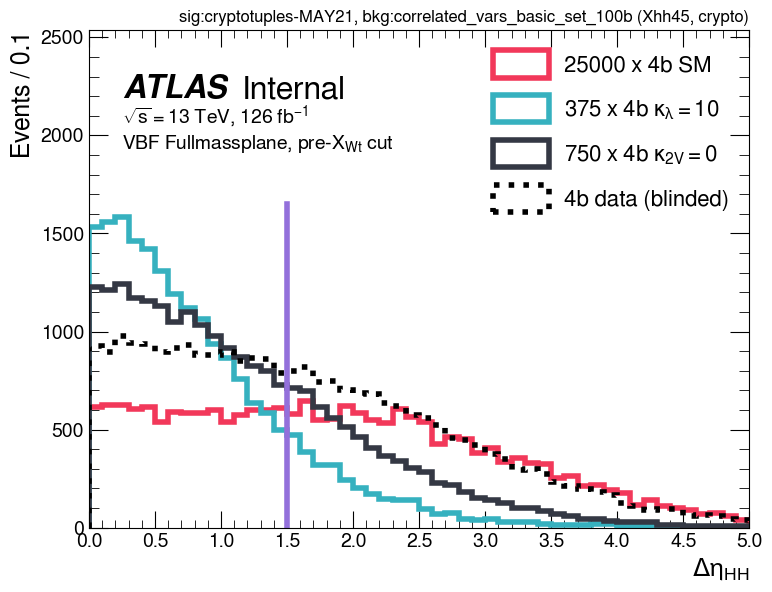
\includegraphics[width=0.45\textwidth]{figures/nr-int-note/category/V3/dEta_hh_VBF_fmp_sig_4bdata_allyears}
	\label{fig:vbf-detahh-4bdata}
	}
	\subfloat[SR with reweighted 2b background estimate.]{ 
		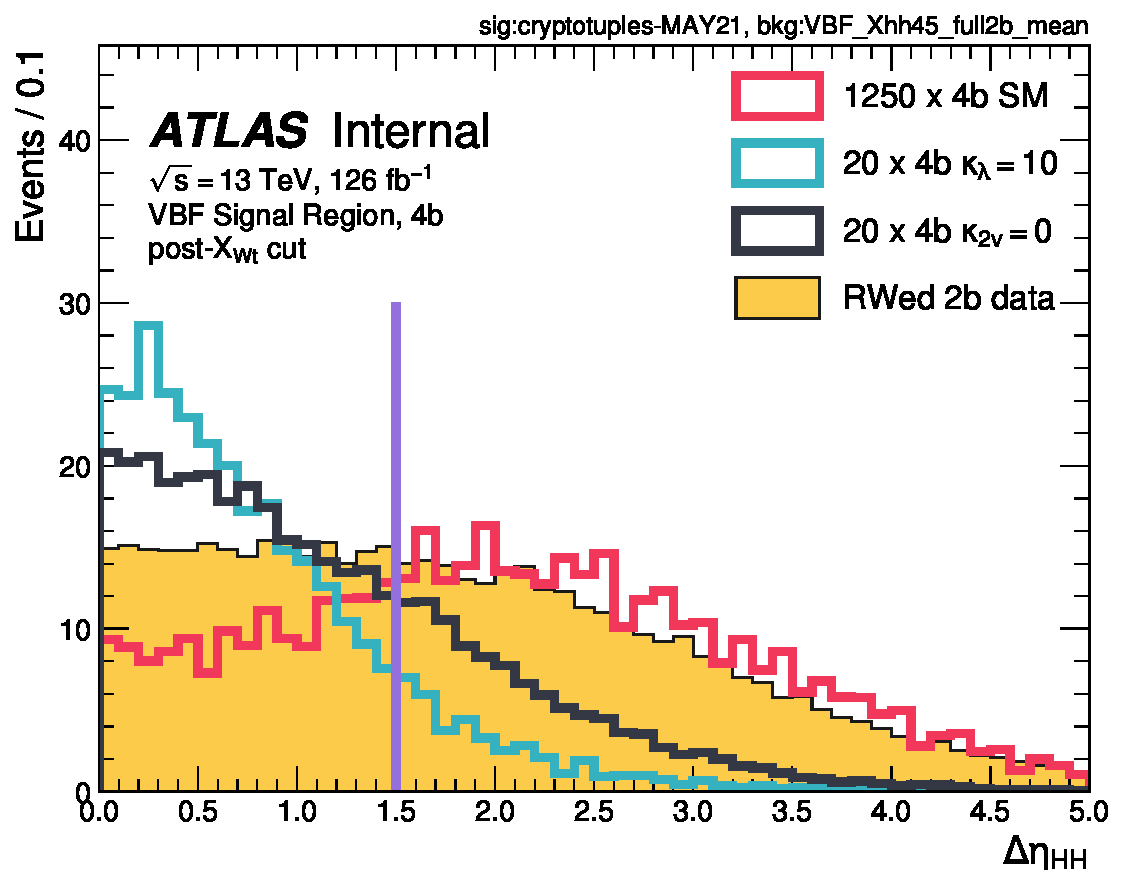
\includegraphics[width=0.45\textwidth]{figures/nr-int-note/category/V3/dEta_hh_VBF_sr_sig_bkg_allyears}
	\label{fig:vbf-detahh-bkg}
	}
	\caption{Distributions of the difference in pseudorapidity of the two reconstructed Higgs bosons ($\deta$) for signal Monte Carlo simulation, data and the background estimate in the VBF channel. The categorisation boundary is shown as a straight purple line at 1.5. The lefthand plot, Figure \ref{fig:vbf-detahh-4bdata}, shows the pre-$X_{wt}$ cut distributions for three key couplings -- $\kappa_{\lambda} = 10$, $\kappa_{2V} = 0$ and the Standard Model prediction -- alongside the 4b data distribution excluding events in the Signal Region. The righthand plot, Figure \ref{fig:vbf-detahh-bkg}, shows the post-$X_{wt}$ cut distributions for the same couplings alongside the reweighted 2b distribution that is used to estimate the background contribution. All signal distributions have been scaled up as to be visible next to data and reweighted data.}
	\label{fig:vbf-detahh}
\end{figure}

Figure \ref{fig:vbf-mhh-same} shows the reconstructed \HH mass distributions for the aforementioned three key couplings and the reweighted 2b data used to model the background contribution. Again, the signal distributions are scaled as to be visible next to the background estimate. Additionally, the significance of the scaled signal ($\alpha \times S/\sqrt{B}$) in each of the histogram bins is shown. The same signal scaling is used for each coupling across the two categories. This allows the sensitivity in the two categories to be compared. 

Due to the low significance below \SI{400}{\GeV} and poor modelling (\Fig{\ref{fig:Control-Region-1all-4b-8}}), we decided to drop the bins of \mhh < \SI{400}{\GeV} in the fit in both categories.

The significance of the $\kappa_{2V} = 0$ signal in the final bin in both plots in Figure \ref{fig:vbf-mhh-same} is far larger than in those preceeding it. The events in the overflow are placed in the final bin for visual purposes, and this is where the increase in signal, and therefore significance, originates. Separating the overflow into finer bins has the potential to improved results by accounting for information on the differing distribution shapes. However, this is a region low in data statistics, particularly 4b events. The binning used was optimized to account for as much shape information as possible whilst ensuring there were enough statistics in each bin for the asymptotic approximation, which is used to derive results, to hold. 

% SCRIPT: hh4b-plots/notebooks/Category-cut.ipynb

\begin{figure}[h!]
	\centering
	\subfloat[$\deta < 1.5$]{ 
		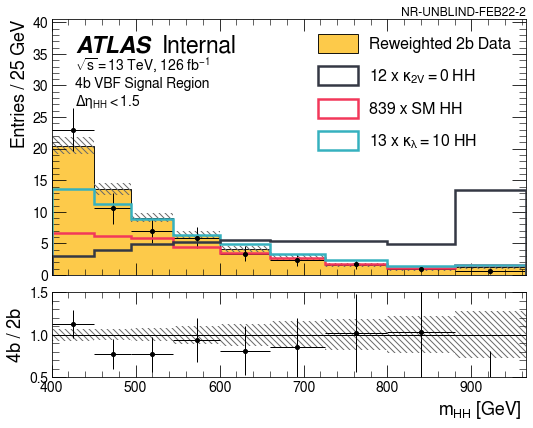
\includegraphics[width=0.45\textwidth]{figures/nr-int-note/category/V4/m_hh_VBF_2_dEta_all_4b_dEta_1.png}%{m_hh_VBF_2_dEta_VBF_all_4b_detahh_lt_1p5_same_scaling.png}
	\label{fig:vbf-mhh-lt-same}
	}
	\subfloat[$\deta \geq 1.5$]{ 
		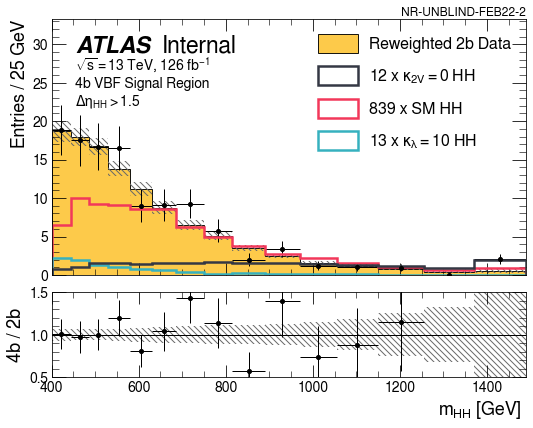
\includegraphics[width=0.45\textwidth]{figures/nr-int-note/category/V4/m_hh_VBF_2_dEta_all_4b_dEta_2.png}%{m_hh_VBF_2_dEta_VBF_all_4b_detahh_gt_1p5_same_scaling.png}
	\label{fig:vbf-mhh-gt-same}
	}
	\caption{Distributions of the reconstructed $m_{HH}$ for signal Monte Carlo simulation and the estimate of the background in each of the two $\deta$ categories in the VBF channel. Distributions for three of the key couplings are shown -- $\kappa_{\lambda} = 10$, $\kappa_{2V} = 0$ and the Standard Model prediction. Additionally, the significance of the scaled signal ($\alpha \times S/\sqrt{B}$) in each of the histogram bins is shown. Events in the underflow and overflow bins are counted in the yields of the initial and final bins respectively. The signals distributions are scaled as to be visible on the plot, and the scaling for each coupling is the same across the two categories.}
	\label{fig:vbf-mhh-same}
\end{figure}

\FloatBarrier
\clearpage



\label{cutflows-tables}

In this section is a breakdown of the yields at the different steps in the analysis event selection (a \textit{cutflow}) for data and important Monte Carlo simulation samples.

Data (2016-18, 126.1 \ifb):

\begin{itemize}
	\item Table \ref{tab:data_ggF_chan_4tag_cutflow}: 4b events in the ggF channel.
	\item Table \ref{tab:data_ggF_chan_2tag_cutflow}: 2b events in the ggF channel.
	\item Table \ref{tab:data_VBF_chan_4tag_cutflow}: 4b events in the VBF channel.
	\item Table \ref{tab:data_VBF_chan_2tag_cutflow}: 2b events in the VBF channel.
\end{itemize}

ggF \HH MC simulation (normalized to 126.1 \ifb):
\begin{itemize}
	\item Tables \ref{tab:mc_ggF_sm_ggF_chan_4tag_cutflow}: 4b events in the ggF channel for SM ggF \HH signal.
	\item Tables \ref{tab:mc_ggF_k10_ggF_chan_4tag_cutflow}: 4b events in the ggF channel for $\kappa_{\lambda} = 10$ ggF \HH signal.
	\item Tables \ref{tab:mc_ggF_sm_VBF_chan_4tag_cutflow}: 4b events in the VBF channel for SM ggF \HH signal.
	\item Tables \ref{tab:mc_ggF_k10_VBF_chan_4tag_cutflow}: 4b events in the VBF channel for $\kappa_{\lambda} = 10$ ggF \HH signal.
\end{itemize}

VBF \HH MC simulation (normalized to 126.1 \ifb):

\begin{itemize}
	\item Tables \ref{tab:mc_VBF_sm_VBF_chan_4tag_cutflow}: 4b events in the VBF channel for SM VBF \HH signal.
	\item Tables \ref{tab:mc_VBF_k10_VBF_chan_4tag_cutflow}: 4b events in the VBF channel for $\kappa_{\lambda} = 10$ VBF \HH signal.
	\item Tables \ref{tab:mc_VBF_k2v0_VBF_chan_4tag_cutflow}: 4b events in the VBF channel for $\kappa_{2V} = 0$ VBF \HH signal.
	\item Tables \ref{tab:mc_VBF_sm_ggF_chan_4tag_cutflow}: 4b events in the ggF channel for SM VBF \HH signal.
	\item Tables \ref{tab:mc_VBF_k10_ggF_chan_4tag_cutflow}: 4b events in the ggF channel for $\kappa_{\lambda} = 10$ VBF \HH signal.
	\item Tables \ref{tab:mc_VBF_k2v0_ggF_chan_4tag_cutflow}: 4b events in the ggF channel for $\kappa_{2V} = 0$ VBF \HH signal.
\end{itemize}

\ttbar MC simulation (normalized to 126.1 \ifb):

\begin{itemize}
	\item Table \ref{tab:ttbar_mc_ttbar_nonallhad_ggF_chan_4tag_cutflow}: 4b events in the ggF channel in \ttbar MC simulation for the non-all hadronic decay mode.
	\item Table \ref{tab:ttbar_mc_ttbar_allhad_ggF_chan_4tag_cutflow}: 4b events in the ggF channel in \ttbar MC simulation for the all hadronic decay mode.
	\item Table \ref{tab:ttbar_mc_ttbar_nonallhad_VBF_chan_4tag_cutflow}: 4b events in the VBF channel in \ttbar MC simulation for the non-all hadronic decay mode.
	\item Table \ref{tab:ttbar_mc_ttbar_allhad_VBF_chan_4tag_cutflow}: 4b events in the VBF channel in \ttbar MC simulation for the all hadronic decay mode.
\end{itemize}

% Tables:
\def\tablesversion{V2}
%data
\begin{table}
\centering
\caption{2016-18 data yields at each step in the analysis event selection for 2b and 4b events in the ggF channel, alongside the ratio of each yield to the initial yield and to the yield for the previous cut. [FEB22-unblind production (For data, expect no changes wrt MAR22)]}
\subfloat[4b data (ggF channel)]{
\centering
\label{tab:data_ggF_chan_4tag_cutflow}
\begin{tabular}{lccc}
\toprule
{} &     Yield &  Yield / Pre-selection &  Yield / Prior cut \\
\midrule
Initial (Unweighted for MC)            &  1.59e+10 &                      - &                  - \\
Pass NTuple Preselection               & 5.697e+08 &                      1 &                  - \\
Trigger                                & 2.807e+08 &                 0.4927 &             0.4927 \\
Trigger Buckets                        &  2.49e+08 &                 0.4371 &             0.8873 \\
ggF channel                            & 2.457e+08 &                 0.4314 &             0.9868 \\
$\ge$ 4 central jets, $\ge$ 2 $b$-tags & 1.806e+08 &                  0.317 &             0.7349 \\
$\ge$ 4 $b$-tags                       & 1.886e+06 &               0.003311 &            0.01045 \\
$|\Delta\eta_{hh}| < 1.5$              & 1.032e+06 &               0.001811 &             0.5469 \\
Top Veto                               & 7.506e+05 &               0.001318 &             0.7276 \\
Signal Region                          & 1.617e+04 &              2.839e-05 &            0.02154 \\
Control Region 2                       & 3.067e+04 &              5.383e-05 &            0.04085 \\
Control Region 1                       & 3.204e+04 &              5.625e-05 &            0.04268 \\
\bottomrule
\end{tabular}
} \ 
\subfloat[2b data (ggF channel)]{
\centering
\label{tab:data_ggF_chan_2tag_cutflow}
\begin{tabular}{lccc}
\toprule
{} &     Yield &  Yield / Pre-selection &  Yield / Prior cut \\
\midrule
Initial (Unweighted for MC)            &  1.59e+10 &                      - &                  - \\
Pass NTuple Preselection               & 5.697e+08 &                      1 &                  - \\
Trigger                                & 2.807e+08 &                 0.4927 &             0.4927 \\
Trigger Buckets                        &  2.49e+08 &                 0.4371 &             0.8873 \\
ggF channel                            & 2.457e+08 &                 0.4314 &             0.9868 \\
$\ge$ 4 central jets, $\ge$ 2 $b$-tags & 1.806e+08 &                  0.317 &             0.7349 \\
2 $b$-tags                             & 1.579e+08 &                 0.2772 &             0.8744 \\
$|\Delta\eta_{hh}| < 1.5$              &  8.27e+07 &                 0.1452 &             0.5238 \\
Top Veto                               &  7.22e+07 &                 0.1267 &              0.873 \\
Signal Region                          & 1.553e+06 &               0.002725 &            0.02151 \\
Control Region 2                       & 2.913e+06 &               0.005113 &            0.04035 \\
Control Region 1                       & 2.983e+06 &               0.005236 &            0.04132 \\
\bottomrule
\end{tabular}
} \ 
\end{table}

\begin{table}
\centering
\caption{2016-18 data yields at each step in the analysis event selection for 2b and 4b events in the VBF channel, alongside the ratio of each yield to the initial yield and to the yield for the previous cut. [FEB22-unblind production (For data, expect no changes wrt MAR22)]}
\subfloat[4b data (VBF channel)]{
\centering
\label{tab:data_VBF_chan_4tag_cutflow}
\begin{tabular}{lccc}
\toprule
{} &     Yield &  Yield / Pre-selection &  Yield / Prior cut \\
\midrule
Initial (Unweighted for MC)            &  1.59e+10 &                      - &                  - \\
Pass NTuple Preselection               & 5.697e+08 &                      1 &                  - \\
Trigger                                & 2.807e+08 &                 0.4927 &             0.4927 \\
Trigger Buckets                        &  2.49e+08 &                 0.4371 &             0.8873 \\
VBF channel                            & 3.295e+06 &               0.005784 &            0.01323 \\
$\ge$ 4 central jets, $\ge$ 2 $b$-tags & 3.157e+06 &               0.005543 &             0.9583 \\
$\ge$ 4 $b$-tags                       & 2.711e+04 &              4.759e-05 &           0.008586 \\
$|\Delta\eta_{hh}| < 1.5$              & 2.711e+04 &              4.759e-05 &                  1 \\
Top Veto                               & 2.175e+04 &              3.818e-05 &             0.8024 \\
Signal Region                          &       502 &              8.812e-07 &            0.02308 \\
Control Region 2                       &       906 &               1.59e-06 &            0.04165 \\
Control Region 1                       &       947 &              1.662e-06 &            0.04354 \\
\bottomrule
\end{tabular}
} \ 
\subfloat[2b data (VBF channel)]{
\centering
\label{tab:data_VBF_chan_2tag_cutflow}
\begin{tabular}{lccc}
\toprule
{} &     Yield &  Yield / Pre-selection &  Yield / Prior cut \\
\midrule
Initial (Unweighted for MC)            &  1.59e+10 &                      - &                  - \\
Pass NTuple Preselection               & 5.697e+08 &                      1 &                  - \\
Trigger                                & 2.807e+08 &                 0.4927 &             0.4927 \\
Trigger Buckets                        &  2.49e+08 &                 0.4371 &             0.8873 \\
VBF channel                            & 3.295e+06 &               0.005784 &            0.01323 \\
$\ge$ 4 central jets, $\ge$ 2 $b$-tags & 3.157e+06 &               0.005543 &             0.9583 \\
2 $b$-tags                             & 2.758e+06 &               0.004842 &             0.8736 \\
$|\Delta\eta_{hh}| < 1.5$              & 2.758e+06 &               0.004842 &                  1 \\
Top Veto                               & 2.469e+06 &               0.004334 &             0.8951 \\
Signal Region                          & 5.873e+04 &              0.0001031 &            0.02379 \\
Control Region 2                       &   1.1e+05 &              0.0001931 &            0.04454 \\
Control Region 1                       & 1.108e+05 &              0.0001946 &            0.04489 \\
\bottomrule
\end{tabular}
} \ 
\end{table}

% ggF sig
\begin{table}
\centering
\caption{ggF \HH MC simulation yields at each step in the analysis event selection for 4b events in the ggF channel normalized to 126.1\ifb, alongside the ratio of each yield to the initial yield and to the yield for the previous cut. [MAR22 production]}
\subfloat[4b SM ggF \HH MC simulation (ggF channel)]{
\centering
\label{tab:mc_ggF_sm_ggF_chan_4tag_cutflow}
\begin{tabular}{lccc}
\toprule
{} &     Yield &  Yield / Pre-selection &  Yield / Prior cut \\
\midrule
%Initial (Unweighted for MC)            & 4.605e+06 &                      - &                  - \\
Pass NTuple Preselection               &     526.6 &                      1 &                  - \\
Trigger                                &       475 &                 0.9019 &             0.9019 \\
Trigger Buckets                        &       419 &                 0.7956 &             0.8821 \\
Multiply FTAG, trig, + JVT SFs         &     381.8 &                  0.725 &             0.9112 \\
ggF channel                            &     376.6 &                 0.7151 &             0.9864 \\
$\ge$ 4 central jets, $\ge$ 2 $b$-tags &     322.4 &                 0.6122 &             0.8561 \\
$\ge$ 4 $b$-tags                       &        86 &                 0.1633 &             0.2668 \\
$|\Delta\eta_{hh}| < 1.5$              &     71.85 &                 0.1364 &             0.8355 \\
Top Veto                               &      60.4 &                 0.1147 &             0.8406 \\
Signal Region                          &      29.1 &                0.05525 &             0.4817 \\
Control Region 2                       &     7.137 &                0.01355 &             0.1182 \\
Control Region 1                       &     11.41 &                0.02166 &             0.1889 \\
\bottomrule
\end{tabular}
} \ 
\subfloat[4b \kl = 10 ggF \HH MC simulation (ggF channel)]{
\centering
\label{tab:mc_ggF_k10_ggF_chan_4tag_cutflow}
\begin{tabular}{lccc}
\toprule
{} &     Yield &  Yield / Pre-selection &  Yield / Prior cut \\
\midrule
%Initial (Unweighted for MC)            & 4.813e+07 &                      - &                  - \\
Pass NTuple Preselection               &      7338 &                      1 &                  - \\
Trigger                                &      6917 &                 0.9427 &             0.9427 \\
Trigger Buckets                        &      6378 &                 0.8692 &              0.922 \\
Multiply FTAG, trig, + JVT SFs         &      5279 &                 0.7194 &             0.8278 \\
ggF channel                            &      5198 &                 0.7084 &             0.9846 \\
$\ge$ 4 central jets, $\ge$ 2 $b$-tags &      4314 &                  0.588 &               0.83 \\
$\ge$ 4 $b$-tags                       &      1002 &                 0.1365 &             0.2322 \\
$|\Delta\eta_{hh}| < 1.5$              &     850.6 &                 0.1159 &             0.8492 \\
Top Veto                               &       569 &                0.07754 &             0.6689 \\
Signal Region                          &     182.7 &                 0.0249 &             0.3211 \\
Control Region 2                       &     66.06 &               0.009003 &             0.1161 \\
Control Region 1                       &     86.18 &                0.01175 &             0.1515 \\
\bottomrule
\end{tabular}
} \ 
\end{table}
\begin{table}
\centering
\caption{ggF \HH MC simulation yields at each step in the analysis event selection for 4b events in the VBF channel normalized to 126.1\ifb, alongside the ratio of each yield to the initial yield and to the yield for the previous cut. [MAR22 production]}
\subfloat[4b SM ggF \HH MC simulation (VBF channel)]{
\centering
\label{tab:mc_ggF_sm_VBF_chan_4tag_cutflow}
\begin{tabular}{lccc}
\toprule
{} &     Yield &  Yield / Pre-selection &  Yield / Prior cut \\
\midrule
%Initial (Unweighted for MC)            & 4.605e+06 &                      - &                  - \\
Pass NTuple Preselection               &     526.6 &                      1 &                  - \\
Trigger                                &       475 &                 0.9019 &             0.9019 \\
Trigger Buckets                        &       419 &                 0.7956 &             0.8821 \\
Multiply FTAG, trig, + JVT SFs         &     381.8 &                  0.725 &             0.9112 \\
VBF channel                            &     5.208 &                0.00989 &            0.01364 \\
$\ge$ 4 central jets, $\ge$ 2 $b$-tags &     5.155 &               0.009789 &             0.9898 \\
$\ge$ 4 $b$-tags                       &      1.14 &               0.002165 &             0.2212 \\
$|\Delta\eta_{hh}| < 1.5$              &      1.14 &               0.002165 &                  1 \\
Top Veto                               &     1.008 &               0.001914 &             0.8838 \\
Signal Region                          &    0.4833 &              0.0009177 &             0.4796 \\
Control Region 2                       &     0.123 &              0.0002336 &              0.122 \\
Control Region 1                       &    0.1703 &              0.0003234 &              0.169 \\
\bottomrule
\end{tabular}
} \ 
\subfloat[4b \kl = 10 ggF \HH MC simulation (VBF channel)]{
\centering
\label{tab:mc_ggF_k10_VBF_chan_4tag_cutflow}
\begin{tabular}{lccc}
\toprule
{} &     Yield &  Yield / Pre-selection &  Yield / Prior cut \\
\midrule
%Initial (Unweighted for MC)            & 4.813e+07 &                      - &                  - \\
Pass NTuple Preselection               &      7338 &                      1 &                  - \\
Trigger                                &      6917 &                 0.9427 &             0.9427 \\
Trigger Buckets                        &      6378 &                 0.8692 &              0.922 \\
Multiply FTAG, trig, + JVT SFs         &      5279 &                 0.7194 &             0.8278 \\
VBF channel                            &     81.14 &                0.01106 &            0.01537 \\
$\ge$ 4 central jets, $\ge$ 2 $b$-tags &     80.22 &                0.01093 &             0.9888 \\
$\ge$ 4 $b$-tags                       &     15.29 &               0.002084 &             0.1906 \\
$|\Delta\eta_{hh}| < 1.5$              &     15.29 &               0.002084 &                  1 \\
Top Veto                               &     11.15 &               0.001519 &              0.729 \\
Signal Region                          &     3.099 &              0.0004223 &              0.278 \\
Control Region 2                       &     1.449 &              0.0001975 &               0.13 \\
Control Region 1                       &     1.851 &              0.0002522 &              0.166 \\
\bottomrule
\end{tabular}
} \ 
\end{table}
% VBF sig
\begin{table}
\small
\centering
\caption{VBF \HH MC simulation yields at each step in the analysis event selection for 4b events in the ggF channel normalized to 126.1\ifb, alongside the ratio of each yield to the initial yield and to the yield for the previous cut. [MAR22 production]}
\subfloat[4b SM VBF \HH MC simulation (ggF channel)]{
\centering
\label{tab:mc_VBF_sm_ggF_chan_4tag_cutflow}
\begin{tabular}{lccc}
\toprule
{} &     Yield &  Yield / Pre-selection &  Yield / Prior cut \\
\midrule
%Initial (Unweighted for MC)            & 8.479e+04 &                      - &                  - \\
Pass NTuple Preselection               &     22.26 &                      1 &                  - \\
Trigger                                &     20.67 &                 0.9287 &             0.9287 \\
Trigger Buckets                        &     18.39 &                 0.8261 &             0.8895 \\
Multiply FTAG, trig, + JVT SFs         &     16.14 &                 0.7251 &             0.8778 \\
ggF channel                            &      13.9 &                 0.6246 &             0.8613 \\
$\ge$ 4 central jets, $\ge$ 2 $b$-tags &     10.75 &                 0.4829 &             0.7731 \\
$\ge$ 4 $b$-tags                       &      1.87 &                0.08402 &              0.174 \\
$|\Delta\eta_{hh}| < 1.5$              &    0.9419 &                0.04232 &             0.5036 \\
Top Veto                               &     0.736 &                0.03307 &             0.7814 \\
Signal Region                          &    0.2352 &                0.01057 &             0.3195 \\
Control Region 2                       &   0.07797 &               0.003503 &             0.1059 \\
Control Region 1                       &    0.1094 &               0.004914 &             0.1486 \\
\bottomrule
\end{tabular}
} \ 
\subfloat[4b \kl = 10 VBF \HH MC simulation (ggF channel)]{
\centering
\label{tab:mc_VBF_k10_ggF_chan_4tag_cutflow}
\begin{tabular}{lccc}
\toprule
{} &     Yield &  Yield / Pre-selection &  Yield / Prior cut \\
\midrule
%Initial (Unweighted for MC)            & 4.827e+06 &                      - &                  - \\
Pass NTuple Preselection               &      1573 &                      1 &                  - \\
Trigger                                &      1465 &                 0.9317 &             0.9317 \\
Trigger Buckets                        &      1303 &                 0.8289 &             0.8896 \\
Multiply FTAG, trig, + JVT SFs         &      1092 &                 0.6941 &             0.8374 \\
ggF channel                            &     955.5 &                 0.6076 &             0.8754 \\
$\ge$ 4 central jets, $\ge$ 2 $b$-tags &     756.5 &                  0.481 &             0.7917 \\
$\ge$ 4 $b$-tags                       &     134.5 &                0.08551 &             0.1778 \\
$|\Delta\eta_{hh}| < 1.5$              &     109.4 &                0.06954 &             0.8132 \\
Top Veto                               &     76.41 &                0.04859 &             0.6988 \\
Signal Region                          &     25.19 &                0.01602 &             0.3297 \\
Control Region 2                       &     8.892 &               0.005654 &             0.1164 \\
Control Region 1                       &     11.42 &               0.007262 &             0.1495 \\
\bottomrule
\end{tabular}
} \ 
\subfloat[4b \kvv = 0 VBF \HH MC simulation (ggF channel)]{
\centering
\label{tab:mc_VBF_k2v0_ggF_chan_4tag_cutflow}
\begin{tabular}{lccc}
\toprule
{} &     Yield &  Yield / Pre-selection &  Yield / Prior cut \\
\midrule
Initial (Unweighted for MC)            & 1.331e+06 &                      - &                  - \\
Pass NTuple Preselection               &     626.1 &                      1 &                  - \\
Trigger                                &     513.5 &                 0.8201 &             0.8201 \\
Trigger Buckets                        &     444.6 &                   0.71 &             0.8658 \\
Multiply FTAG, trig, + JVT SFs         &     405.2 &                 0.6471 &             0.9114 \\
ggF channel                            &     334.4 &                 0.5341 &             0.8254 \\
$\ge$ 4 central jets, $\ge$ 2 $b$-tags &     260.5 &                  0.416 &             0.7788 \\
$\ge$ 4 $b$-tags                       &     65.23 &                 0.1042 &             0.2504 \\
$|\Delta\eta_{hh}| < 1.5$              &     46.37 &                0.07405 &             0.7108 \\
Top Veto                               &      43.1 &                0.06884 &             0.9296 \\
Signal Region                          &     22.97 &                0.03669 &              0.533 \\
Control Region 2                       &     4.854 &               0.007752 &             0.1126 \\
Control Region 1                       &      8.26 &                0.01319 &             0.1916 \\
\bottomrule
\end{tabular}
} \ 
\end{table}
\begin{table}
\small
\centering
\caption{VBF \HH MC simulation yields at each step in the analysis event selection for 4b events in the VBF channel normalized to 126.1\ifb, alongside the ratio of each yield to the initial yield and to the yield for the previous cut. [MAR22 production]}
\subfloat[4b SM VBF \HH MC simulation (VBF channel)]{
\centering
\label{tab:mc_VBF_sm_VBF_chan_4tag_cutflow}
\begin{tabular}{lccc}
\toprule
{} &     Yield &  Yield / Pre-selection &  Yield / Prior cut \\
\midrule
%Initial (Unweighted for MC)            & 8.479e+04 &                      - &                  - \\
Pass NTuple Preselection               &     22.26 &                      1 &                  - \\
Trigger                                &     20.67 &                 0.9287 &             0.9287 \\
Trigger Buckets                        &     18.39 &                 0.8261 &             0.8895 \\
Multiply FTAG, trig, + JVT SFs         &     16.14 &                 0.7251 &             0.8778 \\
VBF channel                            &     2.238 &                 0.1005 &             0.1387 \\
$\ge$ 4 central jets, $\ge$ 2 $b$-tags &     2.223 &                0.09986 &             0.9931 \\
$\ge$ 4 $b$-tags                       &    0.7449 &                0.03347 &             0.3351 \\
$|\Delta\eta_{hh}| < 1.5$              &    0.7449 &                0.03347 &                  1 \\
Top Veto                               &    0.6722 &                 0.0302 &             0.9024 \\
Signal Region                          &    0.3265 &                0.01467 &             0.4857 \\
Control Region 2                       &   0.09092 &               0.004085 &             0.1352 \\
Control Region 1                       &    0.1149 &               0.005164 &              0.171 \\
\bottomrule
\end{tabular}
} \ 
\subfloat[4b \kl = 10 VBF \HH MC simulation (VBF channel)]{
\centering
\label{tab:mc_VBF_k10_VBF_chan_4tag_cutflow}
\begin{tabular}{lccc}
\toprule
{} &     Yield &  Yield / Pre-selection &  Yield / Prior cut \\
\midrule
%Initial (Unweighted for MC)            & 4.827e+06 &                      - &                  - \\
Pass NTuple Preselection               &      1573 &                      1 &                  - \\
Trigger                                &      1465 &                 0.9317 &             0.9317 \\
Trigger Buckets                        &      1303 &                 0.8289 &             0.8896 \\
Multiply FTAG, trig, + JVT SFs         &      1092 &                 0.6941 &             0.8374 \\
VBF channel                            &     136.1 &                0.08651 &             0.1246 \\
$\ge$ 4 central jets, $\ge$ 2 $b$-tags &     135.1 &                0.08589 &             0.9929 \\
$\ge$ 4 $b$-tags                       &     46.14 &                0.02934 &             0.3416 \\
$|\Delta\eta_{hh}| < 1.5$              &     46.14 &                0.02934 &                  1 \\
Top Veto                               &     34.84 &                0.02216 &             0.7551 \\
Signal Region                          &     14.24 &               0.009055 &             0.4087 \\
Control Region 2                       &      4.23 &                0.00269 &             0.1214 \\
Control Region 1                       &      5.03 &               0.003198 &             0.1443 \\
\bottomrule
\end{tabular}
} \ 
\subfloat[4b \kvv = 0 VBF \HH MC simulation (VBF channel)]{
\centering
\label{tab:mc_VBF_k2v0_VBF_chan_4tag_cutflow}
\begin{tabular}{lccc}
\toprule
{} &     Yield &  Yield / Pre-selection &  Yield / Prior cut \\
\midrule
Initial (Unweighted for MC)            & 1.331e+06 &                      - &                  - \\
Pass NTuple Preselection               &     626.1 &                      1 &                  - \\
Trigger                                &     513.5 &                 0.8201 &             0.8201 \\
Trigger Buckets                        &     444.6 &                   0.71 &             0.8658 \\
Multiply FTAG, trig, + JVT SFs         &     405.2 &                 0.6471 &             0.9114 \\
VBF channel                            &     70.74 &                  0.113 &             0.1746 \\
$\ge$ 4 central jets, $\ge$ 2 $b$-tags &      70.3 &                 0.1123 &             0.9939 \\
$\ge$ 4 $b$-tags                       &     27.63 &                0.04412 &              0.393 \\
$|\Delta\eta_{hh}| < 1.5$              &     27.63 &                0.04412 &                  1 \\
Top Veto                               &     26.52 &                0.04236 &             0.9601 \\
Signal Region                          &     17.29 &                0.02761 &             0.6517 \\
Control Region 2                       &     3.074 &                0.00491 &             0.1159 \\
Control Region 1                       &     3.805 &               0.006078 &             0.1435 \\
\bottomrule
\end{tabular}
} \ 
\end{table}
% ttbar
\begin{table}
\centering
\caption{\ttbar MC simulation yields at each step in the analysis event selection for 4b events in the ggF channel normalized to 126.1\ifb, alongside the ratio of each yield to the initial yield and to the yield for the previous cut. [MAY21-crypto production, missing MC SFs eg trigger SF, expect to be about 10\% smaller after applying SFs.]}
\subfloat[4b Non-all hadronic \ttbar MC simulation (ggF channel)]{
\centering
\label{tab:ttbar_mc_ttbar_nonallhad_ggF_chan_4tag_cutflow}
\begin{tabular}{lccc}
\toprule
{} &     Yield &  Yield / Pre-selection &  Yield / Prior cut \\
\midrule
%Initial (Unweighted for MC)            &  1.53e+13 &                      - &                  - \\
Pass NTuple Preselection               & 6.698e+06 &                      1 &                  - \\
Trigger                                & 6.215e+06 &                 0.9279 &             0.9279 \\
Trigger Buckets                        & 5.542e+06 &                 0.8274 &             0.8917 \\
ggF channel                            & 5.488e+06 &                 0.8193 &             0.9903 \\
$\ge$ 4 central jets, $\ge$ 2 $b$-tags & 4.313e+06 &                 0.6439 &             0.7859 \\
$\ge$ 4 $b$-tags                       & 3.424e+04 &               0.005112 &           0.007939 \\
$|\Delta\eta_{hh}| < 1.5$              & 1.989e+04 &               0.002969 &             0.5807 \\
Top Veto                               &  1.07e+04 &               0.001598 &             0.5383 \\
Signal Region                          &     403.5 &              6.024e-05 &             0.0377 \\
Control Region 2                       &     642.3 &               9.59e-05 &               0.06 \\
Control Region 1                       &     734.8 &              0.0001097 &            0.06864 \\
\bottomrule
\end{tabular}
} \ 
\subfloat[4b All hadronic \ttbar MC simulation (ggF channel)]{
\centering
\label{tab:ttbar_mc_ttbar_allhad_ggF_chan_4tag_cutflow}
\begin{tabular}{lccc}
\toprule
{} &     Yield &  Yield / Pre-selection &  Yield / Prior cut \\
\midrule
%Initial (Unweighted for MC)            &  1.53e+13 &                      - &                  - \\
Pass NTuple Preselection               & 6.698e+06 &                      1 &                  - \\
Trigger                                & 6.215e+06 &                 0.9279 &             0.9279 \\
Trigger Buckets                        & 5.542e+06 &                 0.8274 &             0.8917 \\
ggF channel                            & 5.488e+06 &                 0.8193 &             0.9903 \\
$\ge$ 4 central jets, $\ge$ 2 $b$-tags & 4.313e+06 &                 0.6439 &             0.7859 \\
$\ge$ 4 $b$-tags                       & 3.424e+04 &               0.005112 &           0.007939 \\
$|\Delta\eta_{hh}| < 1.5$              & 1.989e+04 &               0.002969 &             0.5807 \\
Top Veto                               &  1.07e+04 &               0.001598 &             0.5383 \\
Signal Region                          &     403.5 &              6.024e-05 &             0.0377 \\
Control Region 2                       &     642.3 &               9.59e-05 &               0.06 \\
Control Region 1                       &     734.8 &              0.0001097 &            0.06864 \\
\bottomrule
\end{tabular}
} \ 
\end{table}

\begin{table}
\centering
\caption{\ttbar MC simulation yields at each step in the analysis event selection for 4b events in the VBF channel normalized to 126.1\ifb, alongside the ratio of each yield to the initial yield and to the yield for the previous cut. [MAY21-crypto production, missing MC SFs eg trigger SF, expect to be about 10\% smaller after applying SFs.]}
\subfloat[4b Non-all hadronic \ttbar MC simulation (VBF channel)]{
\centering
\label{tab:ttbar_mc_ttbar_nonallhad_VBF_chan_4tag_cutflow}
\begin{tabular}{lccc}
\toprule
{} &     Yield &  Yield / Pre-selection &  Yield / Prior cut \\
\midrule
%Initial (Unweighted for MC)            &  1.53e+13 &                      - &                  - \\
Pass NTuple Preselection               & 6.698e+06 &                      1 &                  - \\
Trigger                                & 6.215e+06 &                 0.9279 &             0.9279 \\
Trigger Buckets                        & 5.542e+06 &                 0.8274 &             0.8917 \\
VBF channel                            & 5.383e+04 &               0.008036 &           0.009713 \\
$\ge$ 4 central jets, $\ge$ 2 $b$-tags &  5.25e+04 &               0.007839 &             0.9754 \\
$\ge$ 4 $b$-tags                       &     351.8 &              5.252e-05 &             0.0067 \\
$|\Delta\eta_{hh}| < 1.5$              &     351.8 &              5.252e-05 &                  1 \\
Top Veto                               &     219.2 &              3.272e-05 &              0.623 \\
Signal Region                          &     8.882 &              1.326e-06 &            0.04053 \\
Control Region 2                       &     13.06 &               1.95e-06 &            0.05959 \\
Control Region 1                       &     13.07 &              1.951e-06 &            0.05964 \\
\bottomrule
\end{tabular}
} \ 
\subfloat[4b All hadronic \ttbar MC simulation (VBF channel)]{
\centering
\label{tab:ttbar_mc_ttbar_allhad_VBF_chan_4tag_cutflow}
\begin{tabular}{lccc}
\toprule
{} &     Yield &  Yield / Pre-selection &  Yield / Prior cut \\
\midrule
%Initial (Unweighted for MC)            &  1.53e+13 &                      - &                  - \\
Pass NTuple Preselection               & 6.698e+06 &                      1 &                  - \\
Trigger                                & 6.215e+06 &                 0.9279 &             0.9279 \\
Trigger Buckets                        & 5.542e+06 &                 0.8274 &             0.8917 \\
VBF channel                            & 5.383e+04 &               0.008036 &           0.009713 \\
$\ge$ 4 central jets, $\ge$ 2 $b$-tags &  5.25e+04 &               0.007839 &             0.9754 \\
$\ge$ 4 $b$-tags                       &     351.8 &              5.252e-05 &             0.0067 \\
$|\Delta\eta_{hh}| < 1.5$              &     351.8 &              5.252e-05 &                  1 \\
Top Veto                               &     219.2 &              3.272e-05 &              0.623 \\
Signal Region                          &     8.882 &              1.326e-06 &            0.04053 \\
Control Region 2                       &     13.06 &               1.95e-06 &            0.05959 \\
Control Region 1                       &     13.07 &              1.951e-06 &            0.05964 \\
\bottomrule
\end{tabular}
} \ 
\end{table}


%**598: The ttbar contamination numbers should also be shown in the cutflow section if possible. We should show it before and after the Xwt cut in the SR for 2b, 4b for ggF and VBF**
% This is in section 7.

\clearpage

\subsection{Signal Yields}
\label{subsec:sigYields}

Tables \ref{tab:ggF_4SR_yields} and \ref{tab:VBF_4SR_yields} show the 4b SR yields for ggF and VBF \HH MC simulation in the ggF and VBF SR. Approximately 1--2\% of the overall ggF yield for the various coupling points shown falls in the VBF SR, demonstrating that the additional of the VBF SR does very little to dilute the sensitivity to ggF. A far larger percentage of the overall VBF yield falls in the ggF SR, but the definition of the VBF SR was optimized to maximize significance, resulting in tight cuts that do reject a significant amount signal but reject far more background.

\begin{table}[h]
    \centering
    \caption{Yields in the 4b Signal Region for coupling points of interest for ggF HH Monte Carlo simulation normalized to 126.1\ifb.}
    \label{tab:ggF_4SR_yields}
    \begin{tabular}{lcc}
        \toprule
        Coupling Point & ggF Channel Yield & VBF Channel Yield \\
        \midrule
        {SM} & {35.2} & {0.561} \\
        {$\kappa_{\lambda} = 10$} & {237} & {3.9} \\
    \bottomrule
    \end{tabular}
\end{table}
      
\begin{table}[h]
    \centering
    \caption{Yields in the 4b Signal Region for coupling points of interest for VBF HH Monte Carlo simulation normalized to 126.1\ifb.}
	\label{tab:VBF_4SR_yields}
    \begin{tabular}{lcc}
        \toprule
        Coupling Point & ggF Channel Yield & VBF Channel Yield \\
        \midrule
        {SM} & {0.276} & {0.371} \\
        {$\kappa_{\lambda} = 10$} & {30.4} & {16.4} \\
        {$\kappa_{2V} = 0$} & {25.2} & {18.7} \\
    \bottomrule
    \end{tabular}
\end{table}

\clearpage

\subsection{Non-resonant signal acceptance versus \kl and \kvv}
\label{Non-resonant-signal-acceptance-versus-kl}
\Figrange{\ref{fig:syield_signif_kl}}{\ref{fig:syield_signif_k2v}} show the variation in the 4b SR signal yields and significance ($S/\sqrt{B}$) versus \kvv and \kl respectively. Even though there is more VBF signal in the ggF SR than the VBF SR for the majority of modifier values, the significance is far larger in the VBF SR.

\begin{figure}[h]
	\centering
	\subfloat[Signal yield versus $\kappa_{\lambda}$]{
		\includegraphics[width=0.48\textwidth]{figures/nr-int-note/selection/V2/signal_yield_versus_kl.png}
		\label{fig:sig_yield_kl}
	}
	\subfloat[Significance versus $\kappa_{\lambda}$]{
		\includegraphics[width=0.48\textwidth]{figures/nr-int-note/selection/V2/s_over_sqrtb_versus_kl.png}
		\label{fig:signif_kl}
	}
	\caption{4b Signal Region yield and statistical significance of the VBF and ggF Monte Carlo simulation in the VBF and ggF SRs versus $\kappa_{\lambda}$.
	In the legend, "channel" means SR.
	}
	\label{fig:syield_signif_kl}
\end{figure}

\begin{figure}[h]
	\centering
	\subfloat[Signal yield versus $\kappa_{2V}$]{
		\includegraphics[width=0.48\textwidth]{figures/nr-int-note/selection/V2/signal_yield_versus_k2v.png}
		\label{fig:sig_yield_k2v}
	}
	\subfloat[Significance versus $\kappa_{2V}$]{
		\includegraphics[width=0.48\textwidth]{figures/nr-int-note/selection/V2/s_over_sqrtb_versus_k2v.png}
		\label{fig:signif_k2v}
	}
	\caption{4b Signal Region yield and statistical significance of the VBF Monte Carlo simulation in the VBF and ggF SRs versus $\kappa_{2V}$.
	In the legend, "channel" means SR.
	}
	\label{fig:syield_signif_k2v}
\end{figure}

 \Fig{\ref{fig:accXeff}} shows the corresponding acceptance times efficiency in 1d as a function of the \kl and \kvv variations. 
Then \Fig{\ref{fig:eff-2d}} shows the corresponding acceptance times efficiency in 2d as a function of the \kl and \kvv variations. 

\begin{figure}[h]
	\centering
	\subfloat[Acceptance times efficiency versus \kl]{
		\includegraphics[width=0.48\textwidth]{figures/nr-int-note/selection/V3/accXeff_kl}
		\label{fig:accXeff_kl}
	}
	\subfloat[Acceptance times efficiency \kvv]{
		\includegraphics[width=0.48\textwidth]{figures/nr-int-note/selection/V3/accXeff_k2V}
		\label{fig:accXeff_k2V}
	}
	\caption{4b Signal Region acceptance times efficiency versus \kl and \kvv.}
	\label{fig:accXeff}
\end{figure}


\begin{figure}[h]
	\centering
	\subfloat[VBF selection]{
	    \includegraphics[width=0.7\textwidth]{figures/nr-int-note/selection/V3/VBFefficiency2D-vbf-MC-Signal-Region-all-4b}
	}
	\subfloat[ggF selection]{
	    \includegraphics[width=0.7\textwidth]{figures/nr-int-note/selection/V3/VBFefficiency2D-ggf-MC-Signal-Region-all-4b}
	}
	\caption{4b Signal Region acceptance times efficiency for the VBF SM Monte Carlo simulation in the VBF or ggF selection in \kvv-\kl plane.}
	\label{fig:eff-2d}
\end{figure}

Finally, to visualize our analysis selection as we propagate through the cutflow chain, the plots for acceptance times efficiency as we propagate through the cutflow acceptance are shown in \Fig{\ref{fig:accXeff-cutflow}}. Here we show the categories driving our analysis sensitivity the ggF signal in the ggF channel and the VBF signals in the VBF channel.  In \App{\ref{app:evt-sel}}, \Fig{\ref{fig:accXeff-cutflow-app}} shows the ggF production $\kl$ cutflows in the VBF channel and the VBF production cutflows for the ggF channel.

\begin{figure}[h]
	\centering
	\subfloat[ggF MC: \kl variation]{
		\includegraphics[width=0.48\textwidth]{figures/nr-int-note/selection/V3/acc_x_eff_ggF_kl_ggF_chan_log}
		\label{fig:accXeff_ggF_kl-ggF-sel-cutflow}
	}
	\subfloat[VBF MC: \kl variation]{
		\includegraphics[width=0.48\textwidth]{figures/nr-int-note/selection/V3/acc_x_eff_VBF_kl_VBF_chan_log}
		\label{fig:accXeff_VBF_kl-VBF-sel-cutflow}
	} \\
	\subfloat[VBF MC: \kvv variation]{
		\includegraphics[width=0.48\textwidth]{figures/nr-int-note/selection/V3/acc_x_eff_VBF_k2v_VBF_chan_log}
		\label{fig:accXeff_k2V-cutflow}
	}
	\caption{4b Signal Region acceptance times efficiency.}
	\label{fig:accXeff-cutflow}
\end{figure}


